\RequirePackage[thinlines]{easybmat} %-- muss aufgrund eines Bugs vor etex und tikz geladen werden
\documentclass[a4paper, twoside, headsepline, index=totoc,toc=listof, fontsize=10pt, cleardoublepage=empty, headinclude, DIV=13, BCOR=13mm, titlepage]{scrartcl}
\usepackage{scrtime} % KOMA, Uhrzeit ermoeglicht
\usepackage{scrpage2} % wie fancyhdr, nur optimiert auf KOMA-Skript, leicht andere Syntax
\usepackage{etoolbox}
\usepackage{ifxetex}

%--Farbdefinitionen
%-- muss vor tikz geladen werden
\usepackage[usenames, table, x11names]{xcolor}
\definecolor{dark_gray}{gray}{0.45}
\definecolor{light_gray}{gray}{0.6}

%--Zum Zeichnen
%-- muss vor polyglossia bzw. babel geladen werden
\usepackage{tikz}
\usepackage{tikz-cd}
\usetikzlibrary{external}
\tikzset{>=latex}
\usetikzlibrary{shapes,arrows,intersections}
\usetikzlibrary{calc,3d}
\usetikzlibrary{decorations.pathreplacing,decorations.markings}
\usetikzlibrary{angles}

%-- Konfiguration von tikzexternalize
\tikzexternalize[prefix=tikz/, up to date check=diff]

\ifxetex
\tikzset{external/system call={xelatex \tikzexternalcheckshellescape %-- verwende LuaLaTeX, wegen dynamischer Speicherallokation
    -halt-on-error -interaction=batchmode -jobname "\image" "\texsource"}}
\else
\tikzset{external/system call={pdflatex \tikzexternalcheckshellescape 
    -halt-on-error -interaction=batchmode -jobname "\image" "\texsource"}}
\fi

%-- tikzexternalize fuer tikzcd deaktivieren, da inkompatibel
\AtBeginEnvironment{tikzcd}{\tikzexternaldisable}
\AtEndEnvironment{tikzcd}{\tikzexternalenable}

%-- um Inkompatibilitaeten von quotes und polyglossia bzw. babel zu vermeiden
\tikzset{
  every picture/.append style={
    execute at begin picture={\shorthandoff{"}},
    execute at end picture={\shorthandon{"}}
  }
}
\usetikzlibrary{quotes}
\usepackage{pgfplots}
\pgfplotsset{compat=1.10}



%-- Mathe
\usepackage{mathtools} % beinhaltet amsmath
\mathtoolsset{showonlyrefs, centercolon}
\usepackage{wasysym}
\usepackage{amssymb} %zusätzliche Symbole
\usepackage{latexsym} %zusätzliche Symbole
\usepackage{stmaryrd} %für Blitz
\usepackage{nicefrac} %schräge Brüche
\usepackage{cancel} %Befehle zum Durchstreichen
\usepackage{mathdots}
\DeclareSymbolFont{bbold}{U}{bbold}{m}{n}
\DeclareSymbolFontAlphabet{\mathbbold}{bbold}
\newcommand{\mathds}[1]{\mathbb{#1}} %Um Kompatibilitaet mit frueheren Benutzung von dsfont herzustellen
\newcommand{\ind}{\mathbbold{1}} % charakteristische-Funktion-Eins
\def\mathul#1#2{\color{#1}\underline{{\color{black}#2}}\color{black}} %farbiges Untersteichen im Mathe-Modus

%-- Alles was mit Schrift und XeteX zu tun hat
\ifxetex
    % XeLaTeX
	\usepackage{mathspec} %beinhaltet fontspec 
    \usepackage{polyglossia} %babel-ersatz
    \setmainlanguage[spelling=new,babelshorthands=false]{german}
	\newcommand\glqq{"}
	\newcommand\grqq{"}
	\defaultfontfeatures{Mapping=tex-text, WordSpace={1.4}} %
    \setmainfont[Ligatures=Common, BoldFont={* Bold}, ItalicFont={* Light Italic}]{Source Sans Pro}
	\setsansfont[Scale=MatchLowercase,Ligatures=Common, BoldFont={* Medium}]{Ubuntu}
	\setallmonofonts[Scale=MatchLowercase, ItalicFont={*}]{Consolas} 
	\usepackage{xltxtra}
	\usepackage{fontawesome}
\else
    % default: pdfLaTeX
    \usepackage[ngerman]{babel}
    \usepackage[T1]{fontenc}
    \usepackage[utf8]{inputenc}
	\usepackage{textcomp} %verhindert ein paar Fehler bei den Fonts
    \usepackage[babel=true, tracking=true]{microtype}
	\usepackage{lmodern}
	\renewcommand{\familydefault}{\sfdefault} 
\fi


%--Mixed
\usepackage[neverdecrease]{paralist}
\usepackage[german=quotes]{csquotes}
\usepackage{makeidx}
\usepackage{booktabs}
\usepackage{wrapfig}
\usepackage{float}
\usepackage[margin=10pt, font=small, labelfont=sf, format=plain, indention=1em]{caption}
\captionsetup[wrapfigure]{name=Abb. }
\usepackage{stackrel}
\usepackage{ifthen}
\usepackage{multicol}
\flushbottom

%--Hyphenation
\hyphenation{di-men-si-o-na-le}


%--Unterstreichung
\usepackage[normalem]{ulem}
\setlength{\ULdepth}{1.8pt}

%--Indexverarbeitung
\newcommand{\bet}[1]{\textbf{#1}}
\newcommand{\Index}[1]{\textbf{#1}\index{#1}}
\makeindex
\setindexpreamble{{\noindent \itshape Die \emph{Seitenzahlen} sind mit Hyperlinks zu den entsprechenden Seiten versehen, also anklickbar} \ifxetex \faHandUp\fi \par \bigskip}
\renewcommand{\indexpagestyle}{scrheadings}


%--Marginnote & todonotes
\usepackage{marginnote}
\renewcommand*{\marginfont}{\color{dark_gray} \itshape \footnotesize }
\usepackage[textsize=small]{todonotes}
\makeatletter
\renewcommand{\todo}[2][]{\tikzexternaldisable\@todo[#1]{#2}\tikzexternalenable}
\makeatother

%--Konfiguration von Hyperref pdfstartview=FitH, 
\usepackage[hidelinks, pdfpagelabels,  bookmarksopen=true, bookmarksnumbered=true, linkcolor=black, urlcolor=SkyBlue2, plainpages=false, hypertexnames=false, citecolor=black, hypertexnames=true, pdfauthor={Jannes Bantje}, pdfborderstyle={/S/U}, linkbordercolor=SkyBlue2, colorlinks=false]{hyperref}

\let\orighref\href
\ifxetex
\renewcommand{\href}[2]{\orighref{#1}{#2\,\faExternalLink}}
\renewcommand{\url}[1]{\href{#1}{\nolinkurl{#1}}}
\fi


%--Römische Zahlen
\newcommand{\RM}[1]{\MakeUppercase{\romannumeral #1{}}}

%--Punkte (nach hyperref)
\usepackage{ellipsis}

%%--Abkürzungen etc.
\newcommand{\light}{\text{\Large $\lightning$}}

%-- Definitionen von weiteren Mathe-Befehlen
\DeclareMathOperator{\re}{Re} %Realteil
\DeclareMathOperator{\im}{Im} %Imaginaerteil
\DeclareMathOperator{\id}{id} %identische Abbildung
\DeclareMathOperator{\Sp}{Sp} %Spur
\DeclareMathOperator{\sgn}{sgn} %Signum
\DeclareMathOperator{\alt}{Alt} %Alternierende n-linearFormen
\DeclareMathOperator{\End}{End} %Endomorphismen
\DeclareMathOperator{\Vol}{Vol} %Volumen
\DeclareMathOperator{\dom}{dom} %Domain
\DeclareMathOperator{\Hom}{Hom} %Homomorphismen
\DeclareMathOperator{\bild}{Bild} %Bild
\DeclareMathOperator{\Kern}{Kern }
\DeclareMathOperator{\rg}{rg} %Rang
\DeclareMathOperator{\Rg}{Rg} %Rang
\DeclareMathOperator{\diam}{diam} %Durchmesser
\DeclareMathOperator{\dist}{dist} %Distanz
\DeclareMathOperator{\grad}{grad} %Gradient
\DeclareMathOperator{\dive}{div} %Gradient
\DeclareMathOperator{\rot}{rot} %Rotation
\DeclareMathOperator{\hess}{Hess} %Hesse-Matrix
\DeclareMathOperator{\koker}{Koker} %Kokern
\DeclareMathOperator{\aut}{Aut} %Automorphismen
\DeclareMathOperator{\ord}{ord} %Ordnung
\DeclareMathOperator{\ggT}{ggT} %ggT
\DeclareMathOperator{\kgV}{kgV} %kgV
\DeclareMathOperator{\Gr}{Gr} %Gerade
\DeclareMathOperator{\Kr}{Kr} %Kreis
\DeclareMathOperator{\Char}{char} %Charakteristik
\DeclareMathOperator{\Aut}{Aut} %Automorphismen
\DeclareMathOperator{\D}{D} %formale Ableitung
% \DeclareMathOperator{\mathd}{d} %formale Ableitung
\newcommand{\mathd}{\ensuremath{\mathrm{d}}}
\DeclareMathOperator{\cov}{cov} %Kovarianz
\DeclareMathOperator{\Gal}{Gal} %Galois
\DeclareMathOperator{\supp}{supp} %Träger
\DeclareMathOperator{\Sym}{Sym} %Symmetrische Gruppe
\DeclareMathOperator{\Zyl}{Zyl} %Zylinder
\DeclareMathOperator{\Mod}{Mod} %Moduln
\DeclareMathOperator{\EPK}{EPK} %Einpunktkompaktifizierung
\DeclareMathOperator{\conj}{conj} %Konjugation
\DeclareMathOperator{\ann}{ann} %Annulator
\DeclareMathOperator{\tor}{tor} %Torsionsmodul
\DeclareMathOperator{\Int}{Int} %Interior/Inneres
\DeclareMathOperator{\Br}{Br} %Brauerergruppe
\DeclareMathOperator{\GL}{GL} %allgemeine lineare Gruppe
\DeclareMathOperator{\Tr}{Tr} %Spur/Trace
%\DeclareMathOperator{\op}{op} %entgegengesetzter Ring
\newcommand{\op}{\mathrm{op}}

\newcommand{\Ker}{\ensuremath{\Kern \,}}
\newcommand{\zirkel}{\rotatebox[origin = c]{-90}{$\varangle$}}
\newcommand{\wirkung}{\!\curvearrowright\!}

\newcommand{\oE}{\OE}

%--Beweisende
\newcommand{\bewende}{\ifmmode \tag*{$\square$} \else \hfill $\square$ \fi}

%--Volumen
\newcommand{\vol}[1]{\ensuremath{\Vol_{#1}}}

%--Skalarprodukt
\DeclarePairedDelimiterX\sprod[2]{\langle}{\rangle}{#1\,\delimsize\vert\,#2}

%--Betrag, Gaußklammer
\DeclarePairedDelimiter{\abs}{\lvert}{\rvert}
\DeclarePairedDelimiter{\ceil}{\lceil}{\rceil}

%--Norm
\DeclarePairedDelimiter\doppelstrich{\Vert}{\Vert}
\newcommand{\norm}[2][\relax]{
\ifx#1\relax \ensuremath{\doppelstrich*{#2}}
\else \ensuremath{\doppelstrich*{#2}_{#1}}
\fi}


%--Umklammern
\DeclarePairedDelimiter\enbrace{(}{)}
\DeclarePairedDelimiter\benbrace{[}{]}

%--Mengen
\DeclarePairedDelimiterX\mengenA[1]{\lbrace}{\rbrace}{#1}
\DeclarePairedDelimiterX\mengenB[2]{\lbrace}{\rbrace}{#1\, \delimsize\vert \, #2}

\makeatletter
\newcommand{\set}[2][\relax]{
\ifx#1\relax \ensuremath{
\mengenA*{#2}}
\else \ensuremath{%
  \mengenB*{#1}{#2}}
\fi}
\makeatother


%--offen und abgeschlossen
\newcommand{\off}{\! \stackrel[\text{offen}]{}{\subset} \!}
\newcommand{\abg}{\! \stackrel[\text{abg.}]{}{\subset} \!}

%--Differential
\newcommand{\diff}[2]{\ensuremath{\frac{{\partial #1}}{{\partial #2}} }}
\newcommand{\diffd}[2]{\ensuremath{\frac{\mathrm{d} #1}{\mathrm{d} #2} }}

%--Diagonale Linien für Matrizen
\newcommand\tikzmark[1]{%
  \tikz[overlay,remember picture,baseline] \node [anchor=base] (#1) {};}

\newcommand\MyLine[3][]{%
  \begin{tikzpicture}[overlay,remember picture]
    \draw[#1] (#2.south) -- (#3.north);
  \end{tikzpicture}}
  
%--Jordankasten
\newcommand{\Jord}{ \begin{BMAT}{|ccc|}{|ccc|} %
				0 & & \\ %
				1\tikzmark{z} &  \diagdown & \\ %
				& \tikzmark{u}1 \MyLine[thick]{z}{u} &  0 %
			\end{BMAT}}
			
%--Jordankasten mit Lambda
\newcommand{\JordLa}[1][\empty]{%
	\ifthenelse{\equal{#1}{\empty}}
		{\begin{BMAT}{|ccc|}{|ccc|} %
				\lambda & & \\ %
				1\tikzmark{z} &  \diagdown & \\ %
				& \tikzmark{u}1 \MyLine[thick]{z}{u} &  \lambda  %
			\end{BMAT}}
		{\begin{BMAT}{|ccc|}{|ccc|} %
				\lambda_{#1}  & & \\ %
				1\tikzmark{z} &  \diagdown & \\ %
				& \tikzmark{u}1 \MyLine[thick]{z}{u} &  \lambda_{#1}  %
			\end{BMAT}}}

%--Inhaltsverzeichnis
\usepackage[tocindentauto]{tocstyle}
\usetocstyle{KOMAlike}			

\newcommand{\fach}{Grundlagen der Analysis, Topologie, Geometrie}
\newcommand{\shortFach}{Analysis, Topologie, Geometrie}
\newcommand{\semester}{SoSe 2014}
\newcommand{\homepage}{https://wwwmath.uni-muenster.de/reine/u/topos/lehre/SS2014/AnaTopGeo/anatopgeo.html}

\newcommand{\prof}{Prof.\,Dr.\,Arthur Bartels}


%--Konfiguration von scrheadings
\setheadsepline{1pt}[\color{light_gray}]
\pagestyle{scrheadings}
%\fancyhf[H, F]{}
\clearscrheadfoot

\providecommand{\shortFach}{\fach}
\lehead{ 
\includegraphics[height=0.5 cm,keepaspectratio]{../master/Bilder/Logo_WWU_Muenster_light_gray.pdf}}
\rehead{\rule{0cm}{0.5cm}\footnotesize \sffamily \color{light_gray} Jannes Bantje -- Mitschrift \shortFach}
\lohead{\rule{0cm}{0.5cm} \footnotesize \sffamily \color{light_gray} Stand: \today \; \thistime[:]}
\rohead{
\includegraphics[height=0.5 cm,keepaspectratio]{../master/Bilder/fb10logo_gray.pdf}}


\ofoot[{ \color{dark_gray} \LARGE \sffamily \thepage}]{{ \color{dark_gray} \LARGE \sffamily \thepage}} %hier wir auch der plain Stil bearbeitet!
\automark{section}
\ifoot{ \color{dark_gray} \small \leftmark}

%--Metadaten
\author{Jannes Bantje}
\titlehead{
\includegraphics[height=1.5cm, keepaspectratio]{../master/Bilder/Logo_WWU_Muenster.pdf}%
\hfill 
\includegraphics[height=1.3cm, keepaspectratio]{../master/Bilder/fb10logo.pdf}}
\title{Skript \fach}
\subtitle{Mitschrift der Vorlesung  \enquote{\fach} von \prof}

\publishers{
Aktuelle Version verfügbar bei: \bigskip\\
\normalsize
\begin{minipage}[t]{0.45\textwidth}
	\centering{
\includegraphics[width=3cm, keepaspectratio]{../master/Bilder/qr_github.pdf} \medskip\\
	
\includegraphics[height=0.4cm, keepaspectratio]{../master/Bilder/github_octo.pdf} 
	
\includegraphics[height=0.4cm, keepaspectratio]{../master/Bilder/GitHub_Logo.pdf} (inklusive Sourcecode)\\
	{\small\url{https://github.com/JaMeZ-B/latex-wwu}}}
\end{minipage}
\hfill
\begin{minipage}[t]{0.45\textwidth}
	\centering{
	
\includegraphics[width=3cm, keepaspectratio]{../master/Bilder/qr_btsync.pdf} \medskip\\
	
\includegraphics[height=0.4cm, keepaspectratio]{../master/Bilder/bt_sync_logo.pdf} 
	{\large \textbf{Bittorrent} Sync} \\
	\texttt{B6WH2DISQ5QVYIRYIEZSF4ZR2IDVKPN3I}
	}
\end{minipage}
}


\begin{document}
\maketitle
\pagenumbering{Roman}
\begin{abstract}
\section*{Vorwort --- Mitarbeit am Skript}
Dieses Dokument ist eine Mitschrift aus der Vorlesung \enquote{\fach, \semester}, gelesen von \prof. Der Inhalt entspricht weitestgehend dem Tafelanschrieb. Für die
Korrektheit des Inhalts übernehme ich keinerlei Garantie! Für Bemerkungen und Korrekturen -- und seien es nur Rechtschreibfehler -- bin ich sehr dankbar. 
Korrekturen lassen sich prinzipiell auf drei Wegen einreichen: 
\begin{itemize}
	\item Persönliches Ansprechen in der Uni, Mails an \orighref{mailto:j.bantje@wwu.de}{j.bantje@wwu.de} (gerne auch mit annotieren PDFs) 
	\item \emph{Direktes} Mitarbeiten am Skript: Den Quellcode poste ich auf GitHub (siehe oben), also stehen vielfältige Möglichkeiten der Zusammenarbeit zur Verfügung:
	Zum Beispiel durch Kommentare am Code über die Website und die Kombination Fork + Pull Request. Wer sich verdient macht oder ein Skript zu einer Vorlesung, die 
	ich nicht besuche, beisteuern will, dem gewähre ich auch Schreibzugriff.
	
	Beachten sollte man dabei, dass dazu ein Account bei \url{github.com} notwendig ist, der allerdings ohne Angabe von persönlichen Daten angelegt werden kann. 
	Wer bei GitHub (bzw. dem zugrunde liegenden Open-Source-Programm \enquote{\texttt{git}}) -- verständlicherweise -- Hilfe beim Einstieg braucht, dem helfe ich gerne 
	weiter. Es gibt aber auch zahlreiche empfehlenswerte Tutorials im Internet\footnote{zB. \url{https://try.github.io/levels/1/challenges/1}, ist auf Englisch, aber dafür 
	interaktives LearningByDoing}.
	\item \emph{Indirektes} Mitarbeiten: \TeX-Dateien per Mail verschicken. 
	
	Dies ist nur dann sinnvoll, wenn man einen ganzen Abschnitt ändern möchte (zB. einen alternativen Beweis geben), da ich die Änderungen dann per Hand einbauen muss!
\end{itemize}
\section*{Vorlesungshomepage}
{\small \url{\homepage}}
\end{abstract}
\tableofcontents
\cleardoubleoddemptypage

\pagenumbering{arabic}
\setcounter{page}{1}

\section{Topologische Räume} % (fold)
\label{sec:1}

\subsection[Definition: Metrischer Raum]{Definition} % (fold)
\label{sub:11}
Ein \Index{metrischer Raum} $(X,d)$ ist eine Menge $X$ mit einer Abbildung $d: X \times X \to [0,\infty)$ mit folgenden Eigenschaften:
\begin{enumerate}[(i)]
	\item $\forall x,y \in X : d(x,y) = d(y,x) $
	\item $\forall x,y \in X : d(x,y)=0 \iff x=y$
	\item $\forall x,y,z \in X : d(x,z) \le d(x,y) + d(y,z)$ \hfill (Dreiecksungleichung)
\end{enumerate}
% subsection 11 (end)

\subsection[Definition: Norm auf einem $\mathds{R}$-Vektorraum]{Definition} % (fold)
\label{sub:12}
Sei $V$ ein $\mathds{R}$-Vektorraum. Eine \Index{Norm} auf $V$ ist eine Abbildung $\norm{.} : V \to [0,\infty)$ mit folgenden Eigenschaften:
\begin{enumerate}[(i)]
	\item $\forall v \in V, \lambda  \in \mathds{R} : \norm{\lambda  \cdot v} = \abs{\lambda}  \cdot \norm{v}  $
	\item $\forall v,w \in V : \norm{v+w} \le \norm{v} + \norm{w} $ \hfill (Dreiecksungleichung)
	\item $\forall v \in V : \norm{v} = 0 \iff v=0$
\end{enumerate} 
Durch $d(v,w) := \norm{v-w} $ erhalten wir eine Metrik auf $V$.
% subsection 12 (end)

\subsection[Beispiel: Normen auf $\mathds{R}^n$]{Beispiel} % (fold)
\label{sub:13}
Auf $\mathds{R}^n$ gibt es verschiedene Normen und damit auch verschiedene Metriken: Für $x= \begin{psmallmatrix}
	x_1 \\ \vdots \\ x_n
\end{psmallmatrix} \in \mathds{R}^n$
\begin{enumerate}[(i)]
	\item $\norm[2]{x} = \sqrt{\sum_{i=1}^{n} x_i^2}  $
	\item $\norm[1]{x}  = \sum_{i=1}^{n} \abs{x_i} $
	\item $\norm[\infty]{x} = \max \set[\abs{x_i} ]{i=1, \ldots , n}  $
\end{enumerate}
% subsection 13 (end)

\subsection[Beispiele für Metriken]{Beispiele} % (fold)
\label{sub:14}
\begin{enumerate}[(i)]
	\item \[
		S^1 := \set[z \in \mathds{C}]{\abs*{z} = 1 } 
	\]
	mit $d(z,z') := \min \set[\abs*{\theta} ]{\theta \in \mathds{R} : z = e^{i \theta} z'} $
	\item Ist $X$ ein metrischer Raum und $A$ eine Teilmenge von $X$, so wird $A$ durch die Einschränkung der Metrik auf $A$ zu einem metrischen Raum. Wir sagen dann $A$ ist 
	ein Unterraum von $X$.
	\item Sei $X$ eine beliebige Menge. Durch
	\[
		d(x,y) := \begin{cases}
			0, &\text{ falls } x=y\\
			1, &\text{ falls } x \not= y
		\end{cases}
	\]
	wir auf $X$ eine Metrik (die \Index{diskrete Metrik}) definiert.
	\item Sei $p$ eine Primzahl. Jedes $x \not= 0 \in \mathds{Q}$ lässt sich eindeutig schreiben als $x = \frac{a}{b} p^n$ mit $n,a,b \in \mathds{Z}, b \not= 0$ und $a,b,p$
	paarweise teilerfremd. Dann heißt
	\[
		\abs*{x}_p := p^{-n} 
	\]
	der \bet{$p$-adische Betrag}\index{p-adischer Betrag@$p$-adischer Betrag} von $x$, $(\abs*{0}_p := 0 )$. Durch $d_p(x,y) := \abs*{x-y}_p $ erhält man die $p$-adische
	 Metrik auf $\mathds{Q}$. 
\end{enumerate}
% subsection 14 (end)

\subsection[Definition: Isometrie und Stetigkeit]{Definition} % (fold)
\label{sub:15}
Seien $(X,d_X)$ und $(Y,d_Y)$ zwei metrische Räume. Eine Abbildung $f : X \to Y$ heißt eine \Index{Isometrie}, falls gilt:
\[
	\forall x,x' \in X : d_Y \enbrace[\big]{f(x), f(x')} = d_X (x,x')
\]
$f$ heißt \Index{stetig}, falls für alle $x_0 \in X$ gilt:
\[
	\forall \varepsilon >0 : \exists \delta >0 : d_X(x,x_0) < \delta  \Longrightarrow d_Y \enbrace[\big]{f(x), f(x_0)} < \varepsilon 
\] 
% subsection 15 (end)

\subsection[Definition: offene Teilmenge]{Definition} % (fold)
\label{sub:16}
Eine Teilmenge $U$ eines metrischen Raums $X$ heißt \Index{offen}, falls gilt 
\[
	\forall x \in U \exists \delta  > 0 \text{ mit } B_\delta (x) = \set[y \in X]{d(x,y) < \delta } \subseteq U   
\]
% subsection 16 (end)

\subsection[Lemma: Charakterisierung von Stetigkeit über offene Mengen]{Lemma} % (fold)
\label{sub:17}
Sei $f : X \to Y$  eine Abbildung zwischen metrischen Räumen. Dann sind äquivalent:
\begin{enumerate}[(i)]
	\item $f$ ist stetig
	\item Urbilder (unter $f$) offener Mengen in $Y$ sind offen in $X$. ($\forall U \subseteq Y$ offen ist $f ^{-1}(U) \subseteq X$ offen)
\end{enumerate}
\minisec{Beweis}
Analysis \RM{2}. \bewende
% subsection 17 (end)

\subsection[Definition: Topologischer Raum]{Definition} % (fold)
\label{sub:18}
Ein \Index{topologischer Raum} $(X, \mathcal{O})$ ist eine Menge $X$ zusammen mit einer Familie $\mathcal{O}$ von Teilmengen von $X$ so dass gilt:
\begin{enumerate}[(i)]
	\item $\emptyset, X \in \mathcal{O}$
	\item $U,V \in \mathcal{O} \Longrightarrow U \cap V \in \mathcal{O}$
	\item Ist $I$ eine Indexmenge und $U_i \in \mathcal{O}$ für $i \in I$, so gilt $\bigcup_{i \in I} U_i \in \mathcal{O}$.
\end{enumerate} 
$\mathcal{O}$ heißt dann eine \Index{Topologie} auf $X$. $U \subseteq X$ heißt \Index{offen}, falls $U \in \mathcal{O}$. $A \subseteq X$ heißt \Index{abgeschlossen},
falls $X \setminus A$ offen ist.  
% subsection 18 (end)

\subsection[Beispiele für Topologien]{Beispiele} % (fold)
\label{sub:19}
\begin{enumerate}[(i)]
	\item Jeder metrische Raum wird durch 
	\(
		\mathcal{O} := \set[U \subseteq X]{U \text{ ist offen}} 
	\)
	zu einem topologischen Raum.
	\item Sei $X$ eine beliebige Menge.
	\begin{enumerate}[(i)]
		\item Die \bet{grobe Topologie}\index{Topologie!grobe} ist $\mathcal{O}_{\text{grob}} := \set{\emptyset, X} $
		\item Die \bet{diskrete Topologie}\index{Topologie!diskrete} ist $\mathcal{O}_{\text{diskret}} := \mathcal{P}(X)$
		\item Die \bet{koendliche Topologie}\index{Topologie!koendliche}  ist 
		$\mathcal{O}_{\text{koendl.}} := \set[U \subseteq X]{X \setminus U \text{ endlich}} \cup \set{\emptyset}$
	\end{enumerate}
\end{enumerate}
% subsection 19 (end)

\subsection[Definition: Stetigkeit in topologischen Räumen]{Definition} % (fold)
\label{sub:110}
Eine Abbildung $f :X \to Y$ zwischen topologischen Räumen heißt \Index{stetig}, wenn Urbilder von offener Mengen offen sind.
% subsection 110 (end)

\subsection[Lemma: Kompositionen stetiger Abbildungen sind stetig]{Lemma} % (fold)
\label{sub:111}
Seien $f : X \to Y$, $g : Y \to Z$ stetige Abbildungen. Dann ist auch $g \circ f : X \to Z$ stetig.
\minisec{Beweis}
Sei $U \subseteq Z$ offen. Dann ist $g ^{-1}(U) \subseteq Y$ offen, da $g$ stetig ist. Da auch $f$ stetig ist, gilt 
$\enbrace{g \circ f } ^{-1} (U) = f ^{-1} \enbrace[\big]{g ^{-1} (U)} \subseteq  X$ offen. \bewende
% subsection 111 (end)

\subsection[Definition: Homöomorphismus]{Definition} % (fold)
\label{sub:112}
Seien $X,Y$ topologische Räume. Eine bijektive stetige Abbildung $f : X \to Y$ heißt ein \Index{Homöomorphismus}, falls auch ihre Umkehrabbildung  $f ^{-1} : Y \to X$ 
stetig ist.

Gibt es einen solchen Homöomorphismus, so heißen $X$ und $Y$ \Index{homöomorph} und wir schreiben $X \cong Y$, andernfalls $X \not\cong Y$.
% subsection 112 (end)

\subsection[Beispiele für homöomorphe Mengen]{Beispiel} % (fold)
\label{sub:113}
\begin{enumerate}[(i)]
	\item $(0,1) \cong (0,\infty) \cong (-\infty,0) \cong \mathds{R}$ \hfill (einfach)
	\item $(0,1)\not\cong [0,1) \not\cong [0,1] \not\cong (0,1)$ \hfill (Übung)
	\item $\mathds{R}^n \cong \mathds{R}^m \iff n=m$ \hfill (schwer)
\end{enumerate}
% subsection 113 (end)

\subsection[Definition: Basis der Topologie]{Definition} % (fold)
\label{sub:114}
Sei $X$ ein topologischer Raum. Eine Familie  $\mathcal{U}$ von offenen Teilmengen von $X$ heißt eine \Index{Basis der Topologie}, falls für jede Teilmenge $W \subseteq X$
äquivalent sind:
\begin{enumerate}[(1)]
	\item $W$ ist offen
	\item $\forall x \in W  : \exists U \in \mathcal{U}$ mit $x \in U \subseteq  W \iff W = \bigcup_{\substack{u \in \mathcal{U}  \\ u \subseteq W}} u$ 
\end{enumerate}
Man sagt $X$ erfüllt das \bet{zweite Abzählbarkeitsaxiom}\index{zweites Abzählbarkeitsaxiom}, falls $X$ eine abzählbare Basis der Topologie besitzt.
% subsection 114 (end)

\subsection[Beispiel: Basis der Topologie in einem metrischen Raum]{Beispiel} % (fold)
\label{sub:115}
Sei $X$ ein metrischer Raum. Dann ist $\set[B_\delta (x)]{x \in X, \delta > 0} $ eine Basis der Topologie von $X$. Gibt es eine abzählbare dichte Teilmenge $X_0\subseteq X$,
so ist $\set[B_{1/n}(x)]{x \in X_0, n \in \mathds{N}} $ eine abzählbare Basis der Topologie von $X$ und $X$ erfüllt das zweite Abzählbarkeitsaxiom.
% subsection 115 (end)

\subsection[Proposition: Bedingung, dass eine Familie von Teilmengen eine Topologie ist]{Proposition} % (fold)
\label{sub:116}
Sei $X$ eine Menge und $\mathcal{U} $ eine Familie von Teilmengen von $X$ mit $X = \bigcup_{U \in \mathcal{U} } U$. Dann ist $\mathcal{U} $ genau dann die Basis einer Topologie 
$\mathcal{O}$ auf $X$, wenn $\mathcal{U} $ folgende Bedingungen erfüllt:
\[
	\forall U,V \in \mathcal{U} : \forall x \in U \cap V : \exists W \in \mathcal{U}  \text{ mit } x \in W \subseteq U \cap V \tag*{$(\star)$}
\]
\minisec{Beweis}
Sei $\mathcal{U} $ die Basis der Topologie $\mathcal{O} $ und $U,V \in \mathcal{U} $. $\Rightarrow U,V$ offen, also ist auch $U \cap V$ offen. Da $\mathcal{U} $ eine Basis
der Topologie ist, gibt es zu jedem $x \in U \cap V$ ein $W \in \mathcal{U} $ mit $x \in W \subseteq U \cap V$. Daher gilt $(\star)$  

Sei umgekehrt $(\star)$ erfüllt. Definiere $\mathcal{O} $ durch
\[
	W \in \mathcal{O} :\Longleftrightarrow \forall x \in W : \exists U \in \mathcal{U} : x \in U \subseteq W.  
\]
Dann $\emptyset \in \mathcal{O} $. Wegen $X = \bigcup_{U \in \mathcal{U} } U$ gilt auch $X \in \mathcal{O} $. Weiter ist $\mathcal{O} $ unter Vereinigungen abgeschlossen.
Seien $W_1, W_2 \in \mathcal{O} $. Sei $x \in W_1 \cap W_2$. Dann gilt
\begin{align*}
	x \in W_1, W_1 \text{ offen } &\Rightarrow  \exists U_1 \in \mathcal{U} : x \in U_1 \subseteq W_1 \\
	x \in W_2, W_2 \text{ offen } &\Rightarrow \exists U_2 \in \mathcal{U} : x \in U_2 \subseteq W_2 
\end{align*}
Also $x \in U_1 \cap U_2$. Mit $(\star)$ folgt: $\exists W \in \mathcal{U} $ mit $x \in W \subseteq U_1 \cap U_2 \subseteq W_1 \cap W_2$. \bewende
% subsection 116 (end)

\subsection[Bemerkung: Eindeutigkeit von Proposition \ref{sub:116}]{Bemerkung} % (fold)
\label{sub:117}
Die Topologie $\mathcal{O}$ in der Proposition \ref{sub:116} wird eindeutig durch $\mathcal{U}$ bestimmt.
% subsection 117 (end)

\subsection[Beispiel: Topologie der punktweisen bzw. gleichmäßigen Konvergenz]{Beispiel} % (fold)
\label{sub:118}
\begin{itemize}
	\item Sei $\mathds{R}^\mathds{N}$ der $\mathds{R}$-Vektorraum aller reellen Folgen. Für 
	$\delta >0$, $n \in \mathds{N} $, $\alpha_1, \ldots , \alpha_n \in \mathds{R}$ sei
	\[
		U_{n, \delta , \alpha_1, \ldots , \alpha_n} := \set[(x_i)_{i \in \mathds{N}}]{\abs*{x_i - \alpha_i} < \delta \text{ für } i=1, \ldots ,n } 
	\]
	Dann erfüllt $\mathcal{U} := { U_{n, \delta , \alpha_1, \ldots , \alpha_n}}$ die Bedingung $(\star)$ und ist die Basis der \Index{Topologie der punktweisen Konvergenz}.
	\item Sei $\mathcal{C}(\mathds{R},\mathds{R}) $ der $\mathds{R}$-Vektorraum aller stetigen Abbildungen. Zu $[a,b] \subset \mathds{R}$, $\delta >0$, 
	$g : [a,b] \to \mathds{R}$ stetig sei
	\[
		U_{a,b, \delta , g} := \set[f : \mathds{R} \to \mathds{R} \text{ stetig}]{\forall t \in [a,b] : \abs[\big]{f(t)- g(t)}< \delta}. 
	\]
	Dann erfüllt $\mathcal{U} := \set{U_{a,b,\delta ,g}}  $ $(\star)$ und ist die Basis der \Index{Topologie der gleichmäßigen Konvergenz} auf kompakten Intervallen.
\end{itemize}
% subsection 118 (end)

\subsection[Definition: Inneres, Abschluss und Rand]{Definition} % (fold)
\label{sub:119}
Sei $Y$ eine Teilmenge eines topologischen Raums $X$.
\begin{align*}
	\mathring Y &:= \set[y \in Y]{ \exists U \subseteq X \text{ offen mit } y \in U \subseteq Y} \text{ heißt das \Index{Innere} von $Y$} \\ 
	\overline{Y} &:= \set[x \in X]{\forall U \subseteq X \text{ offen mit } x \in U : U \cap Y \not= \emptyset}    \text{ heißt \Index{Abschluss von $Y$} } \\
	\partial Y &:= \overline{Y} \setminus \mathring Y \text{ heißt der \Index{Rand} von $Y$. } 
\end{align*}
% subsection 119 (end)

\subsection[Bemerkung: Gleichungen für Inneres, Abschluss und Rand]{Bemerkung} % (fold)
\label{sub:120}
\begin{enumerate}[1)]
	\item $\mathring Y = X \setminus (\overline{X \setminus Y} )$, $\overline{Y} = X \setminus (X \setminus Y)^\circ$.
	\item $\mathring Y = \bigcup_{\substack{U \subseteq Y \\ U \text{ offen}}} U$ ist offen.
	\item $\overline{Y} = \bigcap\limits_{\substack{A \supseteq Y \\ A \text{ abgeschlossen}}} \! \! \! \! A \enspace$ ist abgeschlossen.
	\item $\partial Y = \overline{Y} \setminus \mathring Y $ ist abgeschlossen.
\end{enumerate}
% subsection 129 (end)

\subsection[Definition: Umgebung]{Definition} % (fold)
\label{sub:121}
Sei $X$ ein topologischer Raum, $x \in X$. $V \subseteq X$ heißt eine \Index{Umgebung} von $x$, falls es $U \subseteq X$ offen gibt mit $x \in U \subseteq V$. Ist $V$
offen, so heißt $V$ eine \Index{offene Umgebung} von $x$. 
% subsection 121 (end)

\subsection[Definition: Hausdorffraum]{Definition} % (fold)
\label{sub:122}
Ein topologischer Raum $X$ heißt \Index{hausdorffsch} (oder eine \Index{Hausdorffraum}), falls es zu jedem Paar $x,y \in X, x \not= y$ offene Umgebungen $U$ von $x$ und
$V$ von $y$ gibt mit $U \cap V = \emptyset$.
\minisec{Beispiel}
\begin{itemize}
	\item Metrische Räume sind hausdorffsch.
	\item Ist $\abs*{X} \ge 2 $ so ist $(X, \mathcal{O}_{\text{grob}} )$ nicht hausdorffsch.
\end{itemize}
% subsection 122 (end)

\subsection[Definition: topologische Mannigfaltigkeit]{Definition} % (fold)
\label{sub:123}
Ein Hausdorffraum $M$, der das zweite Abzählbarkeitsaxiom erfüllt, heißt eine \Index{topologische Mannigfaltigkeit} der Dimension $n$ (oder eine $n$-Mannigfaltigkeit), 
falls er lokal homöomorph zum $\mathds{R}^n$ ist; d.h. $\forall x \in M \exists$ offene Umgebung $U$ von $x$ mit $U \cong \mathds{R}^n$.
% subsection 123 (end)
% section 1 (end)
\newpage

\section{Konstruktion topologischer Räume} % (fold)
\label{sec:2}

\subsection[Definition: Spurtopologie]{Definition} % (fold)
\label{sub:21}
Sei $X$ ein topologischer Raum und $A \subseteq X$ eine Teilmenge. Die \Index{Spurtopologie} auf $A$ besteht aus allen Teilmengen von $A$ der Form $A \cap U$ mit 
$U \subseteq X$ offen. Mit dieser Topologie heißt $A$ ein Unterraum von $X$.

\bet{Achtung:} $U \subseteq A$ offen $\not\Rightarrow 	U \subseteq X$ offen!
% subsection 21 (end)

\subsection[Bemerkung: Stetigkeit durch Verknüpfung mit Inklusion]{Bemerkung} % (fold)
\label{sub:22}
Sei $i : A \to X$ die Inklusion.
\begin{enumerate}[(i)]
	\item $i$ ist stetig.
	\item Ist $Y$ ein weiterer topologischer Raum und $f : Y \to A$ eine Abbildung. Dann gilt:
	\[
		f \text{ stetig } \iff i \circ  f : Y \to X \text{ ist stetig}
	\]
\end{enumerate}
% subsection 22 (end)

\subsection[Definition: Produkttopologie]{Definition} % (fold)
\label{sub:23}
Seien $X,Y$ topologische Räume. Eine Basis für die \Index{Produkttopologie} auf $X \times Y$ ist 
\[
	\mathcal{U} := \set[U \times V]{U \subseteq X \text{ offen }, V \subseteq Y \text{ offen}}. 
\]
% subsection 23 (end)

\subsection[Definition: Produkttopologie mit unendlichen vielen Faktoren]{Definition} % (fold)
\label{sub:24}
Seien $X_i$ für $i \in I$ topologische Räume. Die Produkttopologie auf ihrem Produkt 
\[
	\prod_{i \in I} X_i = \set[(x_i)_{i \in I}]{x_i \in X_i} 
\]
hat als Basis alle Mengen der Form $\prod_{i \in I} U_i$ mit
\begin{enumerate}[1)]
	\item $U_i \subseteq X_i$ ist offen
	\item Für fast alle $i$ ist $U_i = X_i$.
\end{enumerate}
% subsection 24 (end)

\subsection[Bemerkung zur Stetigkeit der Projektionen und Stetigkeit im Produktraum]{Bemerkung} % (fold)
\label{sub:25}
Seien $p_j : \prod_{i \in I} X_i \to X_j$ die Projektionen.
\begin{enumerate}[(i)]
	\item Die $p_j$ sind stetig.
	\item Ist $Y$ ein weiterer topologischer Raum und $f : Y \to \prod_{i \in I} X_i$ eine Abbildung, so gilt: \\
	$f$ ist stetig $\iff \forall j $ ist $f_j := p_j \circ f$ stetig.
\end{enumerate}
% subsection 25 (end)

\subsection[Bemerkung zur üblichen Topologie auf $\mathds{R}^n$]{Bemerkung} % (fold)
\label{sub:26}
Die übliche Topologie auf $\mathds{R}^n = \prod_{i =1}^n \mathds{R}$ stimmt mit der Produkttopologie überein.
% subsection 26 (end)
\newpage

\subsection[Beispiel: Torus]{Beispiel} % (fold)
\label{sub:27}
\tikzsetnextfilename{Torus}
\begin{figure}[h]
	\centering{\begin{tikzpicture}[xscale=0.9, yscale=0.6]
	    \begin{axis}[hide axis, view={40}{50}]
	       \addplot3[surf,
	       colormap/cool,
	       samples=50,
	       domain=0:2*pi,y domain=0:2*pi,
	       z buffer=sort,
		   shader=faceted interp,]
	       ({(2+cos(deg(x)))*cos(deg(y+pi/2))}, 
	        {(2+cos(deg(x)))*sin(deg(y+pi/2))}, 
	        {sin(deg(x))});
	    \end{axis}
	\end{tikzpicture}
	\caption{Der Torus $T^2$, \href{http://tex.stackexchange.com/questions/348/how-to-draw-a-torus}{Quelle}}}
\end{figure}
$T^n := \underbrace{S^1 \times \ldots \times S^1}_{n} = \prod_{i=1}^n S1$ heißt der $n$-Torus. Der $n$-Torus ist eine $n$-Mannigfaltigkeit.


% subsection 27 (end)

\subsection[Definition: Homotopie und homotop]{Definition} % (fold)
\label{sub:28}
Seien $X$ und $Y$ topologische Räume und $(f_t)_{t \in [0,1]}$ eine Familie von stetigen Abbildungen $f_t : X \to Y$. Wir sagen, dass die $f_t$ stetig von $t$ abhängen,
falls 
\[
	H : X \times [0,1] \to Y \text{ mit } H(x,t) = f_t(x)
\]
stetig bezüglich der Produkttopologie ist. In diesem Fall heißen $f_0$ und $f_1$ \Index{homotop} und $H$ eine \Index{Homotopie} zwischen $f_0$ und $f_1$. 
\minisec{Beispiel}
Je zwei Abbildungen $f,g : X \to \mathds{R}^n$ sind homotop; eine Homotopie wird gegeben durch $H(x,t) := (1-t)\cdot f(x) + t \cdot g(x)$. Wir werden später sehen, dass 
$\id : S^1 \to S^1$ nicht homotop zu einer konstanten Abbildung ist.
% subsection 28 (end)

\subsection[Definition: Quotiententopologie]{Definition} % (fold)
\label{sub:29}
Sei $X$ ein topologischer Raum, $M$ eine Menge und $q : X \to M$ eine surjektive Abbildung. Die offenen Mengen der \Index{Quotiententopologie} auf $M$ (bezüglich $q$) sind 
alle $U \subseteq M$ für die $q ^{-1} (U ) \subseteq X$ offen ist.
\minisec{Bemerkung}
\begin{enumerate}[(i)]
	\item $q : X \to M$ ist stetig.
	\item Ist $Y$ ein weiterer topologischer Raum und $f : M \to Y$ eine Abbildung, so gilt 
	\[
		f \text{ ist stetig } \iff f \circ q \text{ ist stetig}
	\]
\end{enumerate}
% \faicon{external-link}
\minisec{Bemerkung}
Sei $\sim$ eine Äquivalenzrelation auf dem topologischen Raum $X$. Dann ist die Äquivalenzklassenabbildung $q : X \to \nicefrac{X}{\sim}$, $x \mapsto [x]_\sim$ surjektiv.
Insbesondere wird $\nicefrac{X}{\sim}$ durch die Quotiententopologie zu einem topologischen Raum.

\subsection[Beispiele zur Quotiententopologie]{Beispiele}
\label{sub:210}
$X = [0,1] \times [0,1]$: Definiere 
\begin{enumerate}[(i)]
	\item $(s,t) \sim (s', t') :\Leftrightarrow (s=s' \text{ und } t=t')$ oder $(s=0, s'=1, t=t')$. Dann \marginnote{"Zusammenkleben"{} der Seiten}
	\[
		\nicefrac{X}{\sim} \cong \enspace
		\vcenter{\hbox{\begin{tikzpicture}[yscale=0.2,xscale=0.3]
		%\fill[top color=gray!50!black,bottom color=gray!10,middle color=gray,shading=axis,opacity=0.25] (0,0) circle (2cm and 0.5cm);
		%\fill[left color=gray!50!black,right color=gray!50!black,middle color=gray!50,shading=axis,opacity=0.25] (2,0) -- (2,6) arc (360:180:2cm and 0.5cm) -- (-2,0) arc (180:360:2cm and 0.5cm);
		%\fill[top color=gray!90!,bottom color=gray!2,middle color=gray!30,shading=axis,opacity=0.25] (0,6) circle (2cm and 0.5cm);
		\draw (-2,6) -- (-2,0) arc (180:360:2cm and 0.5cm) -- (2,6) ++ (-2,0) circle (2cm and 0.5cm);
		\draw[densely dashed] (-2,0) arc (180:0:2cm and 0.5cm);
		\end{tikzpicture}}} \enspace
		 \cong \enspace \vcenter{\hbox{\begin{tikzpicture}[scale=0.7]
		 	\draw (0,0) circle[radius=1];
			\draw (0,0) circle[radius=1.3];
			\draw (0,1) -- (0,1.3);
		 \end{tikzpicture}}}
	\]
	\item $(s,t) \sim (s',t') :\Leftrightarrow (s=s' \text{ und }t=t')$ oder $(s=0, s'=1 \text{ und } t=1-t')$. Dann\marginnote{Möbiusband: Verdrehen und dann
	 Zusammenkleben} \\
	\begin{minipage}{\textwidth}
		\captionsetup{type=figure, skip=0pt}
		\centering{
		\[
			\nicefrac{X}{\sim} \enspace\cong  \enspace
			\vcenter{\hbox{\begin{tikzpicture}[yscale=0.5, xscale=0.9]
			\begin{axis}[
			    hide axis,
			    view={40}{40}
			]
			\addplot3 [
			    surf, shader=faceted interp,
			    point meta=x,
			    colormap/greenyellow,
			    samples=70,
			    samples y=5,
			    z buffer=sort,
			    domain=0:360,
			    y domain=-0.5:0.5
			] (
			    {(1+0.5*y*cos(x/2)))*cos(x)},
			    {(1+0.5*y*cos(x/2)))*sin(x)},
			    {0.5*y*sin(x/2)});

			\addplot3 [
			    samples=60,
			    domain=-145:180, % The domain needs to be adjusted manually, depending on the camera angle, unfortunately
			    samples y=0,
			    thick
			] (
			    {cos(x)},
			    {sin(x)},
			    {0});
			\end{axis}
			\end{tikzpicture}}}
		\]
		\caption{Möbius-Band, \href{http://tex.stackexchange.com/questions/118563/moebius-strip-using-tikz}{Quelle}}
		}
	\end{minipage}
	\item Sei $\mathds{R}P^n$ die Menge aller $1$-dimensionalen Unterräume des $\mathds{R}^{n+1}$. Wir erhalten eine surjektive Abbildung 
	\[
		q : \mathds{R}^{n+1}\setminus \set{0} \to \mathds{R}P^n \enspace,  \quad  q(v) := \langle v\rangle>
	\]
	$\mathds{R}P^n$ mit der Quotiententopologie bezüglich $q$ heißt der \Index{reell projektive Raum} der Dimension $n$. Er ist eine $n$-Mannigfaltigkeit. 
	\item Betrachte auf $\mathds{R}$ die Relation $x \sim y :\Leftrightarrow x-y \in \mathds{Q}$. Der Raum der Äquivalenzklassen bezeichnen wir mit 
	$\nicefrac{\mathds{R}}{\mathds{Q}}$. Dann ist $\nicefrac{\mathds{R}}{\mathds{Q}}$ mit der Quotiententopologie nicht hausdorffsch, obwohl $\mathds{R}$ natürlich
	hausdorffsch ist.\\
	(Übung: Die Quotiententopologie auf $\nicefrac{\mathds{R}}{\mathds{Q}}$ ist die grobe Topologie.)
	\item Sei $f : X \to X$ eine stetige Abbildung. Betrachte auf $X \times [0,1]$ die Äquivalenzrelation 
	\[
		(x,t) \sim (x',t') : \Leftrightarrow (x=x' \text{ und } t=t') \text{ oder } (t=0, t'=1 \text{ und } x'= f(x))
	\] 
	Der Quotient $T_f := \nicefrac{X \times [0,1]}{\sim}$ heißt der \Index{Abbildungstorus} von $f$. 
\end{enumerate}
% subsection 29 (end)
% section 2 (end)
\newpage
\section{Konvergenz} % (fold)
\label{sec:3}
\subsection[Definition: Konvergenz in topologischen Räumen]{Definition} % (fold)
\label{sub:31}
Sei $X$ ein topologischer Raum und $(x_n)_{n \in \mathds{N}}$ eine Folge in $X$. Dann sagen wir $(x_n)_{n \in \mathds{N} }$ konvergiert gegen $x \in X$, falls gilt:
Zu jeder offenen Umgebung $V$ von $x$, gibt es $N \in \mathds{N}$, sodass $x_n \in V$ für alle $n \ge N$. Wir schreiben dann $x_n \to x$ oder $x_n \xrightarrow{n \to \infty} x$. $x$ heißt ein Grenzwert von $(x_n)_{n \in \mathds{N}}$.

\minisec{Bemerkung}
Bezüglich der groben Topologie ist jeder Punkt Grenzwert jeder Folge.
\minisec{Beispiel}
Betrachte die Topologie der gleichmäßigen Konvergenz auf kompakten Teilmengen auf dem Raum $\mathcal{C}(\mathds{R},\mathds{R})$. Dann gilt für Folgen 
$(f_n)_{n \in \mathds{N} }$ von stetigen Abbildungen $f_n \in \mathcal{C}(\mathds{R},\mathds{R}) $
\[
	f_n \to f \iff \forall a < b \text{ konvergiert } f_n|_{[a,b]} \to f_{[a,b]} \text{ gleichmäßig.}
\]
% subsection 31 (end)

\subsection{Lemma (Eindeutigkeit von Grenzwerten)} % (fold)
\label{sub:32}
Sei $X$ hausdorffsch. Gilt $x_n \to x$ und $x_n \to y$, so folgt $x=y$.
\minisec{Beweis}
Übung!
% subsection 32 (end)

\subsection[Definition: Gerichtete Menge]{Definition} % (fold)
\label{sub:33}
Eine nichtleere Menge $\Lambda $ mit einer Relation "$\le$"{} heißt \bet{gerichtet}\index{gerichtete Menge}, falls gilt 
\begin{enumerate}[(i)]
	\item $\forall \lambda  \in \Lambda : \lambda  \le \lambda $
	\item $\forall \lambda_1, \lambda_2, \lambda_3 \in \Lambda  : \lambda_1 \le \lambda_2 \wedge \lambda_2 \le \lambda_3 \Rightarrow \lambda_1 \le \lambda_3$
	\hfill (transitiv)
	\item $\forall \lambda_1, \lambda_2 \in \Lambda : \exists \mu : \lambda_1 \le \mu \wedge \lambda_2 \le \mu$
\end{enumerate} 
% subsection 33 (end)

\subsection[Definition: Netz und Konvergenz bezüglich eines Netzes]{Definition} % (fold)
\label{sub:34}
Sei $X$ ein topologischer Raum. Ein \Index{Netz} $(x_\lambda)_{\lambda \in \Lambda }$ in $X$ besteht aus einer gerichteten Menge $\Lambda $ und Elementen 
$x_\lambda \in X$ für $\lambda \in \Lambda $. Für $x \in X$ sagen wir $(x_\lambda )_{\lambda \in \Lambda }$ konvergiert gegen $x$, falls gilt:
\[
	\forall \text{ Umgebungen } U \text{ von } x : \exists \lambda_0 \in \Lambda : \forall \lambda \in \Lambda \text{ mit } 
	\lambda \ge \lambda_0 \text{ gilt } x_\lambda \in U
\]
Wir schreiben dann $x_\lambda \xrightarrow{\lambda  \to \infty} x$ oder $x_\lambda \to x$.
\minisec{Beispiel}
Sei $X$ ein topologischer Raum und $x \in X$. Dann ist $\Lambda := \set[U]{U \text{ ist offene Umgebung von }x} $ gerichtet bezüglich
\[
	U \le V :\Leftrightarrow V \subseteq U
\]
Ist nun $x_U \in U$ für alle $U \in \Lambda $ so $x_U \to x$.
% subsection 34 (end)

\subsection{Lemma (Eindeutigkeit von Grenzwerten)} % (fold)
\label{sub:35}
Sei $X$ hausdorffsch. Gilt $x_\lambda  \to x$ und $x_\lambda \to y$, so folgt $x=y$.
\minisec{Beweis}
Angenommen $x \not= y$. Da $X$ hausdorffsch ist existiert eine Umgebung $U$ von $x$ und $V$ von $y$ mit $U \cap V = \emptyset$. 
\begin{gather}
	x_\lambda \to x \Rightarrow \exists \lambda_U : x_\lambda  \in U : \forall \lambda \ge \lambda_U \\
	x_\lambda \to y \Rightarrow \exists \lambda_V : x_\lambda  \in V : \forall \lambda \ge \lambda_V 
\end{gather}
Sei nun $\mu \in \Lambda$ mit $\mu \ge \lambda_U$, $\mu \ge \lambda_V$. Dann folgt $x_\mu \in U\cap V = \emptyset$ \light \bewende
% subsection 35 (end)

\subsection[Definition: Teilnetz]{Definition} % (fold)
\label{sub:36}
Sei $(x_\lambda)_{\lambda  \in \Lambda}$ ein Netz in $X$. Ein \Index{Teilnetz} von $(x_\lambda )_{\lambda  \in \Lambda}$ ist eine gerichtete Menge $\Lambda'$ mit einer
Abbildung $f : \Lambda' \to \Lambda$, so dass gilt
\begin{enumerate}[i)]
	\item $\lambda'_1 \le \lambda'_2 \Rightarrow f(\lambda'_1) \le f(\lambda'_2)$ \hfill ($f$ erhält $\le$)
	\item $\forall \lambda \in \Lambda : \exists \lambda' \in \Lambda'$ mit $\lambda  \le f(\lambda' )$ \hfill ($f$ ist kofinal)
\end{enumerate}
Oft schreiben wir $\enbrace*{x_{f(\lambda')}}_{\lambda' \in \Lambda'}$ für ein Teilnetz.
\minisec{Bemerkung}
Ein Teilnetz einer Folge ist \emph{nicht} notwendig eine Teilfolge.
% subsection 36 (end)
% section 3 (end)
\newpage

\section{Kompakte Räume} % (fold)
\label{sec:4}

\subsection[Definition: Offene Überdeckung und Teilüberdeckung]{Definition} % (fold)
\label{sub:41}
Eine Familie $\mathcal{U}$ von offenen Teilmengen von $X$ heißt eine \Index{offene Überdeckung}, falls 
\[
	\bigcup_{U \in \,\mathcal{U}} U = X.
\] 
$\mathcal{V} \subseteq \mathcal{U} $ heißt eine \Index{Teilüberdeckung}, falls immer noch $X \subseteq \bigcup_{V \in \mathcal{V} } V$.
% subsection 41 (end)

\subsection[Definition: Kompaktheit]{Definition} % (fold)
\label{sub:42}
Ein topologischer Hausdorffraum $X$ heißt \Index{kompakt}, wenn jede offene Überdeckung von $X$ eine endliche Teilüberdeckung besitzt.
% subsection 42 (end)

\subsection[Definition: Endliche Durchschnittseigenschaft]{Definition} % (fold)
\label{sub:43}
Eine Familie $\mathcal{A}$ von abgeschlossenen Teilmengen von $X$ hat die \Index{endliche Durchschnittseigenschaft}, wenn für jedes $\mathcal{A}_0 \subseteq \mathcal{A}$ mit
$\abs*{\mathcal{A}_0 } < \infty$ gilt 
\[
	\bigcap_{A \in \mathcal{A}_0 } A \not= \emptyset.
\]
% subsection 43 (end)

\subsection[Lemma: Äquivalenz zur Kompaktheit eines Hausdorffraumes]{Lemma} % (fold)
\label{sub:44}
Sei $X$ ein Hausdorffraum. Dann ist $X$ genau dann kompakt, wenn gilt: Hat eine Familie $\mathcal{A}$ von abgeschlossenen Teilmengen von $X$ die endliche 
Durchschnittseigenschaft, so gilt 
\[
	\bigcap_{A \in \mathcal{A}} A \not= \emptyset
\]
\minisec{Beweis}
Ist $\mathcal{U}$ eine Familie von offenen Teilmengen, so ist $\mathcal{A} := \set[X \setminus U]{U \in \mathcal{U}}$ eine Familie von abgeschlossenen Teilmengen. Ist
umgekehrt $\mathcal{A}$ eine Familie von abgeschlossenen Teilmengen, so ist 
\[
	\mathcal{U} := \set[X \setminus A]{A \in \mathcal{A} } 
\]
eine Familie von offenen Teilmengen.
Dann gilt: 
\begin{itemize}
	\item $\mathcal{U}$ hat eine endliche Teilüberdeckung $\iff \mathcal{A}$ hat nicht die endliche Durchschnittseigenschaft.
	\item $\mathcal{U}$ ist eine Überdeckung $\iff \bigcap_{A \in \mathcal{A} }A = \emptyset$. \bewende
\end{itemize}
% subsection 44 (end)

\subsection[Satz: Charakterisierung von Kompaktheit durch konvergente Teilnetze]{Satz} % (fold)
\label{sub:45}
Sei $X$ ein Hausdorffraum. Dann sind äquivalent:
	\begin{enumerate}[1)]
		\item $X$ ist kompakt.
		\item Jedes Netz in $X$ besitzt ein konvergentes Teilnetz.
	\end{enumerate}
\minisec{Beweis}
\begin{description}
	\item["1) $\Rightarrow $ 2)":] Sei $(x_\lambda )_{\lambda  \in \Lambda}$ ein Netz in $X$. Für $\lambda  \in \Lambda$ sei 
	$A_\lambda := \overline{\set[x_{\lambda'}]{\lambda '  \ge \lambda } }$. \\
	Behauptung($\star$): $\mathcal{A} := \set[A_\lambda ]{\lambda  \in \Lambda}  $ hat die endliche Durchschnittseigenschaft. Sei 
	$\mathcal{A}_0 \subseteq \mathcal{A}$ endlich, also
	$\mathcal{A}_0 = \set[A_\lambda ]{\lambda \in \Lambda_0}  $ für ein $\Lambda_0 \subseteq \Lambda$ endlich. Da $\Lambda$ gerichtet ist, gibt es $\lambda \in \Lambda$ mit
	$\lambda \ge \mu$ für alle $\mu \in \Lambda_0$. Es folgt $x_\lambda \in \set[x_{\lambda'}]{\lambda ' \ge \mu} $ für alle $\mu \in \Lambda_0$. Insbesondere folgt aus 
	\[
		x_\lambda \in \bigcap_{\mu \in \Lambda_0} A_\mu
	\]
	Da $X$ kompakt ist, folgt aus $(\star)$
	\[
		\bigcap_{\lambda  \in \Lambda} A_\lambda \not= \emptyset.
	\]
	Wähle $x \in \bigcap_{\lambda  \in \Lambda} A_\lambda$. Sei $\mathcal{U} $ die Menge aller offenen Umgebungen von $x$. Sei 
	\[
		\Lambda_\mathcal{U} := \set[(\lambda , U)]{\lambda \in \Lambda, x_\lambda \in U \in \mathcal{U}}
	\]
	Durch $(\lambda , U) \le (\lambda', U') :\Leftrightarrow \lambda \le \lambda'$ und $U \supseteq U'$ wird $\Lambda_\mathcal{U}$ zu einer gerichteten Menge: 
	Sei $(\lambda_1, U_1)$ und $(\lambda _2, U_2) \in \Lambda_\mathcal{U}$. Sei $U := U_1 \cap U_2$. Wähle $\lambda \in \Lambda$ mit $\lambda \ge \lambda_1$ und 
	$\lambda  \ge \lambda_2$. Da $x \in A_\lambda = \overline{\set[x_{\lambda'}]{\lambda' \ge \lambda}} $ gibt es $\lambda' \ge \lambda $ mit $x_{\lambda'} \in U$.
	Also $(\lambda', U) \in \Lambda_\mathcal{U} $ und $(\lambda_1, U_1)$, $(\lambda_2, U_2) \le (\lambda', U)$. Mit $x_{(\lambda , U)} = x_\lambda $ ist 
	$(x_{\lambda , U})_{(\lambda ,U) \in \Lambda_\mathcal{U} }$ das gesuchte Teilnetz.
	\item["2) $\Rightarrow $ 1)":] Sei $\mathcal{A}$ eine Familie von abgeschlossenen Teilmengen mit der endlichen Durchschnittseigenschaft. Sei 
	$\Lambda := \set[\mathcal{A}_0 \subseteq \mathcal{A}  ]{\mathcal{A}_0 \text{ ist endlich} } $. $\Lambda$ ist gerichtet bezüglich 
	$\mathcal{A}_0 \le \mathcal{A}_1  :\Leftrightarrow \mathcal{A}_0 \subseteq \mathcal{A}_1 $. Zu $\mathcal{A}_0 \in \Lambda $ wähle 
	\[
		x_{\mathcal{A}_0 } \in \bigcap_{A \in \mathcal{A}_0 } A \not= \emptyset
	\]
	Sei nun $(x_{f(\lambda )})_{\lambda  \in \Lambda'}$ mit $f : \Lambda' \to \Lambda$ ein konvergentes Teilnetz von $(x_{\mathcal{A}_0 })_{\mathcal{A}_0 \in \Lambda}$.
	Sei $x$ der Grenzwert von $(x_{f(\lambda')})_{\lambda'  \in \Lambda'}$. 
	
	Behauptung: $x \in \bigcap_{A \in \mathcal{A}_0 } A$. \\
	Sei $A \in \mathcal{A}_0 $ und $U = X \setminus A$. Angenommen $x \in U$. Da $U$ eine offene Umgebung von $x$ ist und $x_{f(\lambda')} \to x$ gilt, gibt es 
	$\lambda_0' \in \Lambda$ mit $x_{f(\lambda')} \in U$ für alle $\lambda' \ge \lambda_0'$. Zu $\set{A} \in \Lambda$ gibt es $\mu \in \Lambda'$ mit $f(\mu) \ge \set{A}$. Da
	$\Lambda '$ gerichtet ist, gibt es $\mu' \ge \mu$ und $\mu' \ge \lambda_0'$. Es folgt $A \in f(\mu')$ und damit $x_{f(\mu')} \in A$, aber andererseits 
	$x_{f(\mu')} \in U  = X \setminus A$, da $\mu' \ge \lambda_0'$ \light \bewende
	
\end{description}
% subsection 45 (end)

\subsection[Bemerkung zu Kompaktheit in metrischen Räumen]{Bemerkung} % (fold)
\label{sub:46}
Sei $X$ ein metrischer Raum. Dann sind äquivalent:
	\begin{enumerate}[1)]
		\item $X$ ist kompakt.
		\item Jede Folge in $X$ besitzt eine konvergente Teilfolge.
	\end{enumerate}
% subsection 46 (end)

\subsection{Satz von Tychonov} % (fold)
\label{sub:47}
Sei $(X_i)_{i \in I}$ eine Familie von kompakten topologischen Räumen. Dann ist auch $X : = \prod_{i \in I} X_i$ kompakt.
\minisec{Beweis}
(unter Benutzung der nachfolgenden Punkte)\\
Ist $(x_\lambda )_{\lambda  \in \Lambda}$ ein Netz in $\prod_i X_i$, so besitzt dieses Netz ein universelles Teilnetz $(x_{f(\mu)})_{\mu \in \Lambda'}$.
Für jedes $i$ ist dann $p_i(x_{f(\mu)})_{\mu \in \Lambda'}$ ein universelles Netz in $X_i$ und nach dem Lemma \ref{sub:411} konvergent.
Daher ist $(x_{f(\mu)})_{\mu \in \Lambda'}$ bezüglich der Produkttopologie konvergent
% subsection 47 (end)


\subsection[Beispiel: Metrik auf dem Produkt metrischer Räume, die Produkttopologie induziert]{Beispiel} % (fold)
\label{sub:48}
Seien $(X_i, d_i)_{i \in \mathds{N}}$ kompakte metrische Räume. Dann gibt es eine Metrik $d$ auf $\prod X_i$, so dass die zugehörige Topologie die Produkttopologie ist.
(Übung)
\minisec{Beweis}
Sei $p_j : \prod_i X_i \to X_j$ die Projektion auf den $j$-ten Faktor. Sei $(x_n)_{n \in \mathds{N}}$ eine Folge in $\prod_i X_i$. Wähle induktiv 
$\mathds{N}= N_0 \supseteq N_1 \supseteq N_2 \supseteq \ldots $ mit 
\begin{enumerate}[(i)]
	\item $\abs*{N_i} = \infty $
	\item $\enbrace*{p_i(x_n)}_{n \in N_i} $ ist eine konvergente Folge in $X_i$.
\end{enumerate}
(Dies ist möglich, da $X_i$ kompakt ist.) Wähle nun $n_k \in N_k$ induktiv, so dass $n_k > n_{k-1}$. Dann ist $\enbrace*{x_{n_k}}_{k \in \mathds{N}} $ eine Teilfolge von
$(x_n)_{n \in \mathds{N}}$. Für $i \in \mathds{N}$ ist $\enbrace*{p_i\enbrace[\big]{x_{n_k}}}_{k \in \mathds{N}, k \ge i}$ eine Teilfolge der konvergenten Folge 
$(p_i(x_n))_{n \in N_i}$ und daher konvergent. Damit konvergiert auch $\enbrace*{p_i \enbrace*{x_{n_k}} }_{k \in \mathds{N}} $ für jedes $i$. Daher konvergiert 
$(x_{n_k})_{k \in \mathds{N}}$ punktweise, also in der Produkttopologie (Übung). \bewende
 % subsection 48 (end)
 
\subsection[Definition: Netze immer wieder und schließlich in $A$]{Definition} % (fold)
\label{sub:49}
Sei $(x_\lambda)_{\lambda  \in \Lambda}$ ein Netz in $X$ und $A \subseteq X$. Wir sagen $(x_\lambda )_{\lambda  \in \Lambda}$ ist \Index{immer wieder in} $A$, falls gilt:
\[
	\forall \lambda \in \Lambda : \exists \mu \in \Lambda \text{ mit } \mu \ge \lambda \text{ und } x_\mu \in A
\]  
Wir sagen $(x_\lambda )_{\lambda  \in \Lambda}$ ist \Index{schließlich in} $A$, falls gilt 
\[
	\exists \lambda  \in \Lambda : \forall \mu \in \Lambda \text{ mit } \mu \ge \lambda \text{ gilt } x_\mu \in A
\] 
\minisec{Bemerkung}
$x_\lambda  \to X \iff$ Für jede Umgebung $U$ von $x$ ist $x_\lambda $ schließlich in $U$.
% subsection 49 (end)

\subsection[Definition: Universelles Netz]{Definition} % (fold)
\label{sub:410}
Ein Netz $(x_\lambda )_{\lambda  \in \Lambda}$ in $X$ heißt \bet{universell}\index{Netz!universell}, falls für jede Teilmenge $A \subseteq X$ gilt: Entweder ist 
$(x_\lambda )_{\lambda \in \Lambda}$ schließlich in $A$ \emph{oder} schließlich in $X \setminus A$.
\minisec{Bemerkung}
\begin{itemize}
	\item Ist $(x_\lambda )_{\lambda  \in \Lambda}$ universell und immer wieder in $A$, dann ist $(x_\lambda )_{\lambda  \in \Lambda}$ schließlich in $A$.
	\item Ist $(x_\lambda )_{\lambda  \in \Lambda}$ ein universelles Netz in $X$ und $f : X \to Y$ eine Abbildung, so ist auch 
	$\enbrace*{f(x_\lambda )}_{\lambda \in \Lambda} $ ein universelles Netz in $Y$.
\end{itemize}
% subsection 410 (end)

\subsection[Lemma: Universelle Netze konvergieren in kompakten Räumen]{Lemma} % (fold)
\label{sub:411}
Ist $X$ kompakt und $(x_\lambda)_{\lambda  \in \Lambda}$ ein universelles Netz in $X$, so konvergiert $(x_\lambda )_{\lambda  \in \Lambda}$ in $X$.
\minisec{Beweis}
Sei $X$ kompakt und $(x_\lambda )_{\lambda  \in \Lambda}$ ein universelles Netz in $X$. Angenommen $(x_\lambda )_{\lambda  \in \Lambda}$ konvergiert nicht in $X$. Dann
gibt es zu jedem $x \in X$ genau eine offene Umgebung $U_x$ von $x$, so dass $(x_\lambda )_{\lambda  \in \Lambda}$ nicht schließlich in $U_x$ ist. Da 
$(x_\lambda )_{\lambda  \in \Lambda}$ universell ist, ist $(x_\lambda )_{\lambda  \in \Lambda}$ schließlich in $X \setminus U_x$.
Da $X= \bigcup_{x \in X} U_x$ und $X$ kompakt ist, gibt es $x_1, \ldots , x_k \in X$ mit $X= U_{x_1} \cup \ldots \cup U_{x_k}$. Für jedes $i \in \set{1, \ldots, k} $ sei
$\lambda_i \in \Lambda$ mit $x_\mu \in X \setminus U_{x_i}$ für $\mu \ge \lambda_i$. Sei nun $\mu \in \Lambda$ mit $\mu  \ge \lambda_i$ für $i=1, \ldots ,k$. Es folgt
\[
	x_\mu \in \bigcap_{i=1}^k (X \setminus U_{x_i}) = X \setminus \enbrace*{\bigcup_{i=1}^k U_{x_i}} = X \setminus X = \emptyset \enspace \lightning \bewende 
\]
% subsection 411 (end)

\subsection[Proposition: Jedes Netzt besitzt universelles Teilnetz]{Proposition} % (fold)
\label{sub:412}
Jedes Netz besitzt ein universelles Teilnetz.
\minisec{Beweis}
Sei $(x_\lambda )_{\lambda  \in \Lambda}$ ein Netz in $X$. Sei 
\[
	\mathfrak{M} := \set[\mathfrak{B} \subseteq \mathcal{P}(X) ]{
	\begin{array}{ll}
		(1) & B \in \mathfrak{B} \Rightarrow (x_\lambda )_{\lambda  \in \Lambda} \text{ ist immer wieder in } B \\
		(2) & B, B' \in \mathfrak{B} \Rightarrow B \cap B' \in \mathfrak{B}
	\end{array}
	} 
\]
Dann ist $\set{X} \in \mathfrak{M}$, insbesondere $\mathfrak{M} \not= \emptyset$. Ist $\mathfrak{M}_0 \subseteq \mathfrak{M}$ mit 
\[
	\mathfrak{B}, \mathfrak{B}' \in \mathfrak{M}_0 \Rightarrow \mathfrak{B} \subseteq \mathfrak(B)' \text{ oder } \mathfrak{B'} \subseteq \mathfrak{B}
\]
so gilt $\bigcup_{\mathfrak{B \in \mathfrak{M}_0}} \mathfrak{B} \in \mathfrak{M}$. Nach dem Zornschen Lemma enthält $\mathfrak{M}$ ein maximales Element $\mathfrak{B}$.
Da $\mathfrak{B}$ maximal ist, ist $X \in \mathfrak{B}$. Sei 
\[
	\Lambda' := \set[(B,\lambda )]{B \in \mathfrak{B}, \lambda \in \Lambda, x_\lambda  \in B}. 
\]
Durch $(B,\lambda ) \le (B', \lambda ') :\Leftrightarrow B \supseteq B', \lambda  \le \lambda '$ wird $\Lambda'$ gerichtet.

Behauptung: $(x_\lambda )_{(B,\lambda)  \in \Lambda'}$ ist universell. \\
\minisec{Hilfssatz}
Sei $(x_\lambda )_{(B,\lambda)  \in \Lambda'}$ immer wieder in $S$. Dann gilt $S \in \mathfrak{B}$. \\
Beweis: Wir zeigen: $\mathfrak{B}^+ := \mathfrak{B} \cup \set[S \cap B]{B \in \mathfrak{B}}  \in \mathfrak{M}$. Da $\mathfrak{B}$ maximal ist und 
$\mathfrak{B} \subseteq \mathfrak{B}^+$ folgt $\mathfrak{B} = \mathfrak{B}^+$ und $S \in \mathfrak{B}^+ =\mathfrak{B}$. 
Offenbar erfüllt $\mathfrak{B}^+$ (2). Es bleibt (1) zu zeigen.

Da $\mathfrak{B} \in \mathfrak{M}$ bleibt zu zeigen: $\forall B \in \mathfrak{B}$ ist $(x_\lambda )_{(\lambda \in \Lambda}$ immer wieder in $B \cap S$. Sei 
$\lambda \in \Lambda$. Gesucht ist nun $\mu \ge \lambda $ mit $x_\mu \in B \cap S$. Da $B \in \mathfrak{B} \in \mathfrak{M}$ gibt es $\lambda ' \in \Lambda$, 
$\lambda ' \ge \lambda $ mit $x_{\lambda'} \in B$. Also $(B, \lambda') \in \Lambda'$. Da $(x_\lambda )_{(B,\lambda)  \in \Lambda'}$ immer wieder in $S$ ist, gibt es
\[
	\Lambda' \ni (A, \mu) \ge (B,\lambda ') \tag{$\star$}
\]
mit $x_{\mu} \in S$. Da $(A,\mu) \in \Lambda'$ ist $x_\mu \in A \stackrel{(\star)}{\subseteq} B$. Sei $S \subseteq X$. Ist $(x_\lambda )_{(B,\lambda)  \in \Lambda'}$
weder schließlich in $S$ noch schließlich in $X \setminus S$, so ist $(x_\lambda )_{(B,\lambda)  \in \Lambda'}$ immer wieder in $S$ und immer wieder in $X \setminus S$.
Mit dem Hilfssatz folgt $S, X \setminus S \in \mathfrak{B} \Rightarrow \emptyset = S \cap (X \setminus S) \in \mathfrak{B}$ \light \bewende

\subsection[Definition: Vektorraum der beschränkten Abbildungen]{Definition} % (fold)
\label{sub:413}
Sei $\ell^\infty(\mathds{Z}) $ der $\mathds{R}$-Vektorraum aller beschränkten Abbildungen $f : \mathds{Z} \to \mathds{R}$.
\[
	\norm[\infty]{f} := \sup \set[\abs*{f(n)} ]{n \in \mathds{Z}}  
\]
ist eine Norm auf $\ell^\infty(\mathds{Z})$.
% subsection 413 (end)

\subsection{Satz (Mittelbarkeit von $\mathds{Z}$)} % (fold)
\label{sub:414}
Es gibt eine Abbildung $M : \ell^\infty(\mathds{Z}) \to \mathds{R} $ mit
\begin{enumerate}[a)]
	\item $M$ ist $\mathds{R}$-linear
	\item $M$ ist positiv: $f \ge 0 \Rightarrow M(f) \ge 0$
	\item $M(\ind) =1$ für $\ind: \mathds{Z} \to \mathds{R}$ mit $\ind(n)=1$ für alle $n \in \mathds{Z}$
	\item $M$ ist $\mathds{Z}$-invariant: Für $f \in \ell^\infty(\mathds{Z}) $ sei $T f \in \ell^\infty(\mathds{Z})$ mit $(T f) (n) = f(n+1)$, dann gilt $M(f)= M(T f)$.
\end{enumerate}
\minisec{Beweis}
Sei $\mathfrak{M} := \set[M : \ell^\infty(\mathds{Z}) \to \mathds{R}]{M \text{ erfüllt a), b), c)}} $. Sei $M_n \in \mathfrak{M}$ mit 
$M_n(f) = \frac{1}{n+1} \sum_{i=0}^{n} f(i) $. Dann gilt für $f \in \ell^\infty(\mathds{Z})$
\begin{align*}
	M_n(f)= M_n(T f) = \frac{1}{n+1} \sum_{i=0}^{n}  f(i) - T f(i) &= \frac{1}{n+1} \sum_{i=0}^{n} \enbrace[\big]{f(i)- f(i+1) } \\
	&=   \frac{1}{n+1} \enbrace[\big]{f(0)- f(n+1)} 
\end{align*}
Es folgt $\abs*{M_n(f) - M_n(T f)} \le \frac{2 \cdot \norm[\infty]{f} }{n+1}$. Wir konstruieren nun eine kompakte Topologie auf $\mathfrak{M}$, dann können wir anschließend
ein konvergentes Teilnetz der Folge $(M_n)_{n \in \mathds{N}}$ betrachten. Sei 
\[
	X := \prod_{f \in \ell^\infty(\mathds{Z})} \big[{- \norm[\infty]{f}}, \norm[\infty]{f} \big]
\]
Aus a), b), c) folgt für $f \in \ell^\infty(\mathds{Z})$, $M \in \mathfrak{M}$ $M(f) \in \big[{- \norm[\infty]{f}}, \norm[\infty]{f}\big]$. Mittels 
\[
	\mathfrak{M} \ni M \mapsto \enbrace[\big]{M(f)}_{f \in \ell^\infty(\mathds{Z})} \in X 
\]
wird $\mathfrak{M}$ zu einem abgeschlossenen Unterraum von $X$. $\mathfrak{M}$ ist 
kompakt bezüglich der Produkttopologie auf $X$, also bezüglich punktweiser Konvergenz.

Sei nun $\alpha : \Lambda \to \mathds{N}$, sodass $M_{\alpha(\lambda)} \to M \in \mathfrak{M}$ (existiert da $\mathfrak{M}$ kompakt). Es folgt
\[
	\forall f \in \ell^\infty(\mathds{Z}) : M_{\alpha(\lambda )}(f) \to M(f) 
\]
Wegen $M_{\alpha(\lambda )}(f) - M_{\alpha(\lambda )}(T f) \xrightarrow{\lambda  \to \infty} M(f) - M(T f) $ und
\begin{align*}
	\abs*{M_{\alpha(\lambda )}(f) - M_{\alpha(\lambda )}(T f)} \le \frac{2 \cdot \norm[\infty]{f} }{\alpha(\lambda )+1} \to 0  
\end{align*}
folgt $M(f) = M(T f)$ für alle $f \in \ell^\infty(\mathds{Z})$. \bewende
% subsection 414 (end)
% section 4 (end)
\newpage

\section{Kompaktifizierungen} % (fold)
\label{sec:5}

\subsection[Definition: Kompaktifizierung]{Definition} % (fold)
\label{sub:51}
Sei $X$ ein topologischer Raum. Ein kompakter Raum $\overline{X}$ heißt eine \Index{Kompaktifizierung} von $X$, falls er $X$ als offenen, dichten Unterraum enthält. 
(Oft heißt $\partial X := \overline{X} \setminus X $ der Rand der Kompaktifizierung)
% subsection 51 (end)

\subsection[Beispiele für Kompaktifizierungen]{Beispiele} % (fold)
\label{sub:52}
\begin{enumerate}[(i)]
	\item $(-1,1) \subseteq [-1,1]$
	\item $\mathring D^n := \set[x \in \mathds{R}^n]{\norm[2]{x} < 1 } \subseteq D^n = \set[x \in \mathds{R}^n]{\norm[2]{x} \le 1 }  $. Für $n=2$:
	\[
		\tikz[baseline=-0.5]{\draw[dashed, fill=LightBlue2] (0,0) circle[radius=0.5];} \enspace\subseteq \enspace
		\tikz[baseline=-0.5]{\draw[fill=LightBlue2!70] (0,0) circle[radius=0.5];}
	\]
	$\partial D^n = S^{n-1} := \set[x \in \mathds{R}^n]{\norm[2]{x} = 1 } $
	\item $f : \mathds{R}^n \to \mathring D^n$, $f(x) := \frac{x}{1+ \norm[2]{x}} $ ist ein Homöomorphismus. Daher können wir $\mathds{R}^n$ zu
	\[
		\overline{\mathds{R}^n} := \mathds{R}^n \dot\cup (S^{n-1} \times \set{\infty} ) \cong D^n 
	\]
	kompaktifizieren.
	\item Definiere auf $\mathds{R}^n \cup \set{\infty}$ folgende Topologie 
	\[
		\mathcal{O} := \set[U]{U \subseteq \mathds{R}^n \text{ ist offen}} \cup \set[U \cup \{\infty\}]{U \subseteq \mathds{R}^n \text{ offen und } \exists R > 0 : 
		\mathds{R}^n \setminus B_R(0) \subseteq U} 
	\]
	Dann ist $\mathds{R}^n \cup \set{\infty}$ eine weitere Kompaktifizierung von $\mathds{R}^n$. Übung: $\mathds{R}^n \cup \set{\infty} \cong S^n $
\end{enumerate}
% subsection 52 (end)

\subsection[Definition: lokalkompakt]{Definition} % (fold)
\label{sub:53}
Ein Hausdorffraum $X$ heißt \Index{lokalkompakt}, wenn für jedes $x \in X$ und jede offene Umgebung $U$ von $x$ eine kompakte Umgebung $K$ von $x$ existiert mit 
$K \subseteq U$.
% subsection 53 (end)

\subsection[Bespiele für lokalkompakte Hausdorffräume]{Beispiel} % (fold)
\label{sub:54}
\begin{enumerate}[(i)]
	\item $\mathds{R}^n$ ist lokalkompakt: Sei $x \in \mathds{R}^n$ und $U \subseteq \mathds{R}^n$ eine offene Umgebung von $x$. $U$ offen 
	$\Rightarrow \exists \varepsilon >0$ mit $B_\varepsilon(x) \subseteq U$. Es folgt $\overline{B_{\varepsilon/2}}(x) \subseteq B_\varepsilon(x) \subseteq U $. Dann
	ist $\overline{B}_{\varepsilon/2}(x)$ eine kompakte Umgebung von $x$, die in $U$ liegt.
	\item Topologische Mannigfaltigkeiten sind lokalkompakt.
	\item Offene Teilräume von lokalkompakten Räumen sind lokalkompakt.
\end{enumerate}
% subsection 54 (end)

\subsection[Proposition: Offene Teilmengen kompakter Räume sind lokalkompakt]{Proposition} % (fold)
\label{sub:55}
Sei $K$ kompakt und $W \subseteq K$ offen. Dann ist $W$ lokalkompakt. Insbesondere sind kompakte Räume auch lokalkompakt.
\minisec{Beweis}
Sei $x \in W$ und $U$ eine offene Umgebung von $x$ in $W$. $K$ Hausdorff $\Rightarrow \forall y \in K \setminus U$ gibt es offene Umgebungen $V_y$ von $y$ und $W_y$ von $x$
mit $V_y \cap W_y = \emptyset$. Dann ist $\set[V_y]{y \in K \setminus U} $ eine offene Überdeckung von $K \setminus U$. Da mit $K$ auch $K \setminus U$ kompakt ist, gibt es
$Y_0 \subseteq K\setminus U$ endlich mit 
\[
	K\setminus U \subseteq \bigcup_{y \in Y_0} V_y
\]
Nun ist $L := K \setminus \bigcup_{y \in Y_0} V_y$ kompakt. Da $\bigcap_{y \in Y_0} W_y \cap U$ offen ist und 
$\enbrace*{\bigcap_{y \in Y_0} W_y} \cap U \subseteq  L$ ist $L$ eine Umgebung von $x$. \bewende
% subsection 55 (end)

\subsection[Definition: Einpunktkompaktifizierung ($\EPK$)]{Definition} % (fold)
\label{sub:56}
Sei $X$ lokalkompakt. Die \Index{Einpunktkompaktifizierung} ($\EPK$) von $X$ ist $\EPK(X) := X \cup \set{\infty}$ mit der folgenden Topologie:
\[
	U \subseteq X \cup \set{\infty} \text{ offen } :\Leftrightarrow U \subseteq X \text{ ist offen oder } U= (X \setminus K) \cup \set{\infty} \text{ mit } K \subseteq X \text{ kompakt}  
\] 
% subsection 56 (end)

\subsection[Proposition über Eigenschaften der Einpunktkompaktifizierung]{Proposition} % (fold)
\label{sub:57}
$\EPK(X)$ ist kompakt. Ist $X$ nicht kompakt, so ist $\EPK(X)$ eine Kompaktifizierung von $X$.
\minisec{Beweis}
Sei $\mathcal{U}$ eine offene Überdeckung von $\EPK(X)$. Sei $U_0 \in \mathcal{U}$ mit $\infty \in U_0$. Dann existiert $K \subseteq X$ kompakt mit 
$U_0 = (X \setminus K) \cup \set{\infty}$. Da $K$ kompakt ist, gibt es $U_1, \ldots , U_n \in \mathcal{U}$ mit $K \subseteq U_1 \cup \ldots \cup U_n$. Dann ist
$U_0, U_1, \ldots , U_n$ eine endliche Teilüberdeckung von $\EPK(X)$.

Zu zeigen: $\EPK(X)$ ist Hausdorff. Seien $x,y \in \EPK(X), x \not= y$. Gilt $x \not= \infty \not= y$ so gibt es $U,V \subseteq X$ mit $x \in U,  y \in V$ und 
$U\cap V = \emptyset$, da $X$ hausdorffsch ist. Nach Definition sind dann $U,V$ auch offen in $\EPK(X)$. Andernfalls sei o.B.d.A. $x = \infty$. Da $X$ lokalkompakt ist, 
gibt es eine Umgebung $K$ von $y$ mit $K \subseteq X$ kompakt. Dann sind $U := \mathring K$ und $V := (X \setminus K) \cup \set{\infty} $ disjunkte offene Umgebungen von 
$x$ und $y$.

Insgesamt gezeigt: $\EPK(X)$ ist kompakt. Sei $X$ nicht kompakt. Ist $U$ eine Umgebung von $\infty \in \EPK(X)$, so gibt es $K \subseteq X$ kompakt mit 
$U = (X \setminus K) \cup \set{\infty}$. Dann ist $U \cap X = X \setminus K$. Da $X$ nicht kompakt ist, ist $X \not= K$, also $X \setminus K  \not= \emptyset$. 
Daher hat jede Umgebung von $\infty \in \EPK(X)$ einen nicht-trivialen Schnitt mit $X$. Also ist $X  \subseteq \EPK(X)$ dicht. \bewende
% subsection 57 (end)

\subsection[Frage nach Fortsetzungen stetiger Funktionen in der Einpunktkompaktifizierung]{Frage} % (fold)
\label{sub:58}
Sei $f : X \to Y$ stetig, $X,Y$ lokalkompakt. Gibt es dann eine stetige Fortsetzung $\overline{f} : \EPK(X) \to \EPK(Y)$ mit $\overline{f}(\infty) = \infty$?
\minisec{Beispiel}
\begin{enumerate}[(i)]
	\item $f : \mathds{R} \to \mathds{R}$, $f(x) \equiv 0$. Dann ist $\overline{f} : \EPK(\mathds{R}) \to \EPK(\mathds{R}) $ mit 
	\[
		\overline{f} (x) = \begin{cases}
			f(x)=0, &\text{ falls }x \in \mathds{R}\\
			\infty , &\text{ falls } x =\infty
		\end{cases}
	\]
	sicher nicht stetig. Natürlich ist aber $\tilde f : \EPK(\mathds{R}) \to \EPK(\mathds{R})$ mit $\tilde f (x) = 0 \,\forall x \in \EPK(\mathds{R})$ stetig.
	\item $f : \mathds{R} \to \mathds{R}$ mit 
	\[
		f(x) = \begin{cases}
			1, &\text{ falls }x \ge 1\\
			x, &\text{ falls }x \in [0,1] \\
			0, &\text{ falls }x \le 0
		\end{cases}
	\]
	Dann gibt es keine stetige Fortsetzung $\overline{f} : \EPK(\mathds{R}) \to\EPK(\mathds{R})$, denn die Folge $x_n = n$ konvergiert in $\EPK(\mathds{R})$ gegen $\infty$.
	Da $f(x_n) = 1$ $\forall n$ müsste $\overline{f} (\infty) = 1 $ sein. Die Folge $y_n = -n$ konvergiert in $\EPK(\mathds{R})$ auch gegen $\infty$. Da $f(y_n) = 0$
	$\forall n$ müsste $\overline{f} (\infty) = 0 $ sein \light.
\end{enumerate}
% subsection 58 (end)

\subsection[Definition: Eigentliche stetige Abbildung]{Definition} % (fold)
\label{sub:59}
Seien $X$ und $Y$ lokalkompakt. Eine stetige Abbildung $f : X \to Y$ heißt \bet{eigentlich}\index{eigentliche Abbildung}, wenn für jede kompakte Teilmenge 
$K \subseteq Y$ auch $f ^{-1}(K) \subseteq X$ kompakt ist.
% subsection 59 (end)

\subsection[Satz: Charakterisierung von eigentlichen stetigen Abbildungen]{Satz} % (fold)
\label{sub:510}
Seien $X,Y$ lokalkompakt und $f : X \to Y$ stetig. Dann sind äquivalent:
\begin{enumerate}[(1)]
	\item $f$ ist eigentlich
	\item $\overline{f} : \EPK(X) \to \EPK(Y) $ mit 
	\[
		\overline{f} (x) = \begin{cases}
			f(x), &\text{ falls }x \in X\\
			\infty, &\text{ falls } x = \infty
		\end{cases} 
	\]
	ist stetig
\end{enumerate}
\minisec{Beweis}
\begin{description}
	\item["(1)$\Rightarrow$(2)":] Sei $U \subseteq \EPK(Y)$ offen. Ist $\infty \not\in U$, so ist $\bar f^{-1}(U)= f ^{-1}(U)$ offen, da $f$ stetig ist. Ist 
	$\infty \in U$, so gibt es $K \subseteq Y$ mit $U = (X \setminus K) \cup \set{\infty}$. Da $f$ eigentlich ist, ist auch $L := f ^{-1}(K) \subseteq X$ kompakt und
	$\bar f ^{-1} (U) = (X \setminus L) \cup \set{\infty}$ ist offen in $\EPK(X)$.
	\item["(2)$\Rightarrow $(1)":] Sei $K \subseteq Y$ kompakt. Dann ist $U = (Y \setminus K) \cup \set{\infty} \subseteq Y$ offen. Da $\bar f$ stetig ist, ist auch 
	$\bar f ^{-1} (U) = \enbrace*{X \setminus f ^{-1}(K)} \cup \set{\infty}$ offen. Damit ist $f ^{-1}(K) \subseteq X$ kompakt. \bewende  
\end{description}
% subsection 510 (end)
% section 5 (end)
\newpage
\section{Der Approximationssatz von Stone-Weierstraß} % (fold)
\label{sec:6}

\subsection[Definition: Verschwinden stetiger Funktionen im Unendlichen]{Definition} % (fold)
\label{sub:61}
Sei $X$ ein lokalkompakter Raum. Eine stetige Funktion $f : X \to \mathds{R}$ \bet{verschwindet}\index{verschwindende Funktion} im Unendlichen, falls für jedes 
$\varepsilon >0$ 
\[
	K_\varepsilon := \set[x \in X]{\abs{f(x)} \ge \varepsilon} 
\] 
kompakt ist. Die \Index{Algebra} aller solchen Funktionen bezeichnen wir mit $C_0(X)$ und für $f \in C_0 (X) $ setzen wir 
\[
	\norm[\infty]{f} :=  \sup_{x \in X} \abs*{f(x)} = \max_{x \in X} \abs*{f(x)}  
\]
$\norm[\infty]{.} $ ist eine Norm auf $C_0(X)$.
\minisec{Bemerkung} % (fold)
$f : X \to \mathds{R}$ liegt in $C_0(X)$ $\iff \overline{f} : \EPK(X) \to \mathds{R} $ mit $\overline{f}(x) = \begin{cases}
	f(x), &\text{ falls }x \in X\\
	0 , &\text{ falls } x= \infty
\end{cases} $ ist stetig.
% subsection 61 (end)

\subsection[Definition: $\mathcal{B} \subseteq C_0(X)$ trennt $x,y \in X$ streng]{Definition} % (fold)
\label{sub:62}
Sei $\mathcal{B} \subseteq C_0(X) $. Wir sagen, dass $\mathcal{B}$ die Punkte von $X$ \bet{streng trennt}, falls es zu $x,y \in X, x \not= y$ ein $f \in \mathcal{B}$ gibt 
mit $0 \not= f(x) \not= f(y)  \not= 0$.
\minisec{Bemerkung}
Sei $\mathcal{A} \subseteq C_0(X) $ eine Unteralgebra. Gilt
\begin{enumerate}[a)]
	\item $\forall x,y \in X : \exists f \in \mathcal{A}  : f(x) \not= f(y)$
	\item $\forall x \in X : \exists g \in \mathcal{A} : g(x) \not= 0 $
\end{enumerate}
so trennt $\mathcal{A}$ die Punkte von $X$ streng.
\minisec{Beispiel}
Sei $[a,b] \subseteq \mathds{R}$ ein kompaktes Intervall. Sei $\mathcal{A} := \set[x \mapsto p(x)]{p \in R[t]} \subseteq C_0([a,b])$. Dann trennt $\mathcal{A}$ die Punkte 
von $[a,b]$ streng.
% subsection 62 (end)

\subsection{Satz (Stone-Weierstraß)} % (fold)
\label{sub:63}
Sei $X$ ein lokalkompakter Raum und sei $\mathcal{A} \subseteq C_0(X)$ eine Unteralgebra, die die Punkte von $X$ streng trennt. Dann ist $\mathcal{A} \subseteq C_0(X)$
dicht bezüglich $\norm[\infty]{.} $.
\minisec{Beweis (mit Lemma 1, 2, 3)}
Sei $h \in C_0(X)$ beliebig. Sei $\varepsilon>0$ beliebig. Zu zeigen: $\exists f \in \bar{\mathcal{A} } : \norm[\infty]{f- h} < \varepsilon $
\begin{description}
	\item[Schritt 1:] Wir konstruieren für $y \in X$ $f_y \in \bar{\mathcal{A}}$ mit 
	\begin{enumerate}[a)]
		\item $f_y(y) = h(y)$
		\item $f_y(z) \ge h(z) - \varepsilon$ für alle $z \in X$
	\end{enumerate}
	Zu $x \in X$ gibt es nach Lemma 3 (\ref{sub:69}) $g_x \in \mathcal{A}$ mit 
	\[
		g_x(y) = h(y) \quad \text{und} \quad g_x(x) = h(x).
	\]
	Sei $U_x := \set[z \in X]{g_x(z) > h(z) - \varepsilon}$. Da $g_x$ und $h$ stetig sind, ist $U_x$ offen. Da $g_x$ und $h$ in $\infty$ verschwinden, ist 
	$X \setminus U_x$ kompakt.
	Wegen $g_x(x)= h(x)$ ist $x \in U_x$. Zu festem $x_1 \in X$ gibt es dann $x_2, \ldots , x_k$ mit $X \setminus U_{x_1} \subseteq \bigcup_{i=2}^k U_{x_i}$.
	Dann gilt auch 
	\[
		X \subseteq \bigcup_{i=2}^k U_{x_i}
	\]
	$f_y := \max \set{g_{x_1}, \ldots , g_{x_k}}$ ist die gesuchte Funktion. Wegen Lemma 2 (\ref{sub:67}) bzw. der Bemerkung \ref{sub:68} gilt $f_y \in \bar{\mathcal{A}}$.
	\item[Schritt 2:] Konstruktion von $f$. Zu $y \in X$ sei $V_y := \set[z \in X]{f_y(z) < h(z)+ \varepsilon}$. Wieder ist $V_y$ offen, $X\setminus V_y$ kompakt und
	$y \in V_y$. Also gibt es wieder $y_1, \ldots , y_l$ mit $X = \bigcup_{i=1}^l V_{y_i}$. Für $f := \min \set{f_{y_1}, \ldots , f_{y_l}}$ gilt dann
	\[
		h(z) - f(z) = \max_i h(z)- f_{y_i} (z) < \varepsilon
	\]
	da $f_{y_i}(z) \ge h(z) -\varepsilon$ $\overset{\text{a)}}{\Rightarrow } h(z)- f_{y_i}(z) \le \varepsilon$ für jedes $i$.
	Weiter gilt 
	\begin{align*}
		f(z)- h(z) = \min_i f_{y_i}(z)- h(z) < \varepsilon
	\end{align*} 
	nach Definition der $V_{y_i}$. Also $\norm[\infty]{f-h} < \varepsilon $. \bewende
\end{description}
% subsection 63 (end)

\subsection{Satz von Dini} % (fold)
\label{sub:64}
Sei $\enbrace*{f_n : [0,1] \to \mathds{R}}_{n \in \mathds{N}}$ eine punktweise monoton wachsende Folge stetiger Funktionen, die punktweise gegen die stetige Funktion $f$
konvergiert. Dann $f_n \to f$ gleichmäßig, d.h. $\norm[\infty]{f_n -f} \to 0 $.
\minisec{Beweis}
Sei $\varepsilon >0$. Zu jedem $t \in [0,1]$ gibt es $n_t$ mit 
\[
	\forall n\ge n_t : f(t) \ge f_n(t) \ge f_{n_t}(t) \ge f(t) - \varepsilon. 
\]
Da $f$ und $f_{n_t}$ stetig sind,
ist $U_t := \set[{s \in [0,1]}]{f(s) - f_{n_t}(s) < \varepsilon} $ offen. Da $[0,1]$ kompakt ist, gibt es $t_0, \ldots , t_k \in [0,1]$ mit 
\[
	[0,1] = U_{t_0} \cup \ldots \cup U_{t_k}
\]
Für alle $n \ge \max \set{n_{t_0}, \ldots , n_{t_k}} $ folgt
\(
	\norm[\infty]{f_n - f} \le \varepsilon
\). \bewende 
% subsection 64 (end)

\subsection[Lemma 1: Folge reeller Polynome, die gleichmäßig gegen Wurzelfunktion konvergiert]{Lemma 1} % (fold)
\label{sub:65}
Sei $g(t) = \sqrt{t}$ für $t \in [0,1]$. Es gibt eine Folge $(p_n)_{n \in \mathds{N}}$ von reellen Polynomen so dass $p_n \to g$ gleichmäßig auf $[0,1]$ und $p_n(0)=0$.
\minisec{Beweis}
Sei $p_0 \equiv 0$ und für $n > 0$
\[
	p_{n+1} (t) := p_n(t) - \frac{1}{2} \cdot \enbrace[\big]{p_n(t)^2 - t} 
\]
Dann $p_n(0)=0$. Per Induktion nach $n$ zeigen wir: $0 \le p_n(t) \le \sqrt{t}$ für alle $t \in [0,1]$
\begin{description}
	\item[$n=0$] $\checkmark$ 
	\item[$n \mapsto n+1$] \begin{align*}
		p_{n+1}(t) - \sqrt{t} = p_n(t) - \sqrt{t} - \frac{1}{2} \enbrace[\Big]{p_n(t)^2 -t} &= \enbrace*{p_n(t) - \sqrt{t} }- \frac{1}{2} \enbrace*{p_n(t)- \sqrt{t}} 
		\enbrace*{p_n(t) + \sqrt{t}}        \\
		&=\underbrace{\enbrace*{p_n(t) - \sqrt{t}  } }_{\le 0} \underbrace{\Big( 1- \frac{1}{2}\underbrace{(p_n(t) + \sqrt{t}  )}_{\text{IV.: }\le 2 \sqrt{t}  } \Big)}_{\ge 0} 
	\end{align*}
	Also $p_{n+1}(t)- \sqrt{t} \le 0$. Es folgt, dass $p_n(t)$ monoton wachsend ist für jedes $t$. Wegen $p_n(t) \le \sqrt{t}$ existiert $\lim_{ n \to \infty} p_n(t)$
	für $t \in [0,1]$. Es folgt 
	\begin{align*}
		0 = \lim_{ n \to \infty} p_{n+1}(t) - \lim_{ n \to \infty} p_n(t) = \lim_{ n \to \infty} \enbrace[\big]{p_{n+1}(t) - p_n(t)} &= \lim_{ n \to \infty} 
		-\frac{1}{2} \enbrace[\big]{p_n(t)^2 -t  } \\
		&= - \frac{1}{2} \enbrace*{ \enbrace*{\lim_{ n \to \infty} p_n(t)}^2 -t }  
	\end{align*}
	$\Rightarrow \lim_{ n \to \infty} p_n(t) = \sqrt{t}$. Mit Dini (\ref{sub:64}) folgt $p_n \to g$ gleichmäßig. \bewende
\end{description}
% subsection 1 (end)

\subsection[Bemerkung: Komposition mit Polynomen ist auch der Algebra]{Bemerkung} % (fold)
\label{sub:66}
Sei $\mathcal{A} \subseteq C_0(X)$ eine Algebra. Ist $p \in \mathds{R}[t]$ ein Polynom mit $p(0)=0$ und $f \in \mathcal{A}$, so liegt auch $p \circ f \in \mathcal{A}$:
$p= \sum_{i=1}^{n} a_i t^i$. Denn 
\[
	p\enbrace[\big]{f(t)} = \sum_{i=1}^{n} a_i f(t)^i = \enbrace*{\sum_{i=1}^{n} a_i f^i} (t) \in \mathcal{A}. 
\]
% subsection 66 (end)

\subsection[Lemma 2: Betrag von $f \in \mathcal{A}$ liegt in $\bar{\mathcal{A}}$]{Lemma 2} % (fold)
\label{sub:67}
Sei $X$ lokalkompakt, $\mathcal{A} \subseteq C_0(X)$ eine Unteralgebra. Dann gilt: $f \in A \Rightarrow \abs*{f} \in \bar{\mathcal{A}}$ \\
{\color{light_gray} ($\bar{\mathcal{A} }:= $ Abschluss von $\mathcal{A}$ bezüglich $\norm[\infty]{.} $)}
\minisec{Beweis}
Sei $f \in \mathcal{A}$. O.B.d.A. sei $f(X) \subseteq [{-1},1]$. Dann $f(x)^2 \in [0,1]$ für alle $x \in X$. Seien die $p_n$ die Polynome aus Lemma 1 (\ref{sub:65}). Dann
\begin{align*}
	\abs*{p_n \enbrace*{f(x)^2} - \sqrt{f(x)^2}} = \abs*{ p_n \enbrace*{f(x)^2} - \abs*{f(x)}} \xrightarrow{n \to \infty}  0 
\end{align*}
gleichmäßig in $x \in X$. Es folgt $\norm[\infty]{p_n(f^2) - \abs*{f} } \to 0 $. Wegen $f \in \mathcal{A} $ gilt $f^2 \in \mathcal{A}$ und nach \ref{sub:66} $p_n(f^2) \in \mathcal{A}$.
Also $\abs*{f} \in \bar{\mathcal{A}}$. \bewende
% subsection 67 (end)

\subsection[Bemerkung: $\max, \min$ von Funktionen aus $\mathcal{A}$ liegen in $\bar{\mathcal{A}}$]{Bemerkung} % (fold)
\label{sub:68}
\begin{enumerate}[(i)]
	\item Für $f,g \in \mathcal{A}$ liegen 
	\[
		\max(f,g) = \frac{1}{2} \enbrace[\big]{f+g + \abs*{f-g}} \quad , \quad \min(f,g) = \frac{1}{2} \enbrace[\big]{f+g - \abs*{f-g} }  \in \Bar{\mathcal{A}}
	\]
	\item Wegen $\bar{\mathcal{A} } = \bar{\bar{\mathcal{A}}}$ gilt auch 
	$f,g \in \bar{\mathcal{A}} \Rightarrow \min(f,g), \max(f,g) \in \bar{\mathcal{A}}$. 
\end{enumerate}
% subsection 68 (end)

\subsection[Lemma 3: Existenz von $f \in \mathcal{A}$ mit $f(x)=\alpha$, $f(y)=\beta$, wenn $\mathcal{A}$ streng trennt]{Lemma 3} % (fold)
\label{sub:69}
Sei $X$ lokalkompakt, $\mathcal{A} \subseteq C_0(X)$ eine Unteralgebra, die die Punkte von $X$ streng trennt. Zu $x,y \in X$, $x \not= y$, $\alpha, \beta \in \mathds{R}$
gibt es dann $f \in \mathcal{A}$ mit $f(x) = \alpha, f(y) = \beta$.
\minisec{Beweis}
Es gibt $g \in \mathcal{A}$ mit $0 \not= g(x) \not= g(y) \not= 0$. Ansatz: Für $\lambda , \mu \in \mathds{R}$ betrachte $f := \lambda g + \mu g^2$.
\[
	\begin{aligned}
		f(x) &{}= \alpha \\
		f(y) &{}= \beta
	\end{aligned} 
	\iff
	\begin{aligned}
		g(x) \lambda + g(x)^2 \mu &= \alpha \\
		g(y) \lambda + g(y)^2 \mu &= \beta
	\end{aligned} 
\]
Da 
\[
	\det \begin{pmatrix}
		g(x)& g(x)^2 \\
		g(y) & g(y)^2
	\end{pmatrix} = g(x) g(y)^2 - g(y) g(x)^2 = g(x)g(y) \enbrace*{g(y) - g(x)} \not= 0 
\]
gibt es $\lambda , \mu \in \mathds{R}$, sodass das Gleichungssystem eine Lösung hat. \bewende
% subsection 69 (end)
% section 6 (end)
\newpage

\section{Metrisierbarkeit} % (fold)
\label{sec:7}

\subsection[Definition: Metrisierbar]{Definition} % (fold)
\label{sub:71}
Ein topologischer Raum $X$ heißt \Index{metrisierbar}, wenn es eine Metrik auf $X$ gibt, so dass die zugehörige Topologie die Topologie von $X$ ist. 
\minisec{Bemerkung}
Ist $X$ metrisierbar, so gibt es für jedes $x \in X$ eine abzählbare Umgebungsbasis $\mathcal{U}_x$ bei $x$, also eine abzählbare Menge von offenen Umgebungen von $x$,
sodass jede Umgebung von $x$ eine Menge aus $\mathcal{U}_x$ enthält. 
\minisec{Beispiel}
$(X, \mathcal{O}_{\text{dis}})$ ist metrisierbar: $d_{\text{dis}}(x,y) := \begin{cases}
	1, &\text{ falls }x \not= y\\
	0 , &\text{ sonst}
\end{cases}$
% subsection 71 (end)

\subsection[Definition: Normaler Hausdorffraum]{Definition} % (fold)
\label{sub:72}
Ein topologischer Hausdorffraum $X$ heißt \bet{normal}\index{Hausdorffraum!normal}, wenn er die folgende Trennungseigenschaft hat: Sind $A,B \subseteq X$ abgeschlossen mit
$A \cap B = \emptyset$, so gibt es $U,V \subseteq X$ offen mit $A \subseteq U$, $B \subseteq V$ mit $U \cap V = \emptyset$.
\minisec{Bemerkung}
Metrisierbare Räume sind normal. \hfill (Übung) 
% subsection 72 (end)

\subsection{Satz (Urysohn)} % (fold)
\label{sub:73}
Sei $X$ ein normaler Raum, der das zweite Abzählbarkeitsaxiom erfüllt (\ref{sub:114}). Dann ist $X$ metrisierbar.
\minisec{Beweis (mit Urysohns Lemma, \ref{sub:74})}
Sei $\mathcal{U}$ eine abzählbare Basis der Topologie von $X$. Da $X$ normal ist, gibt es zu jedem Paar $U,V \in \mathcal{U}$ mit $\overline{U} \subseteq V $ (also
$\overline{U} \cap X \setminus V = \emptyset $) eine stetige Funktion $f_{U,V} : X \to [0,1]$ mit $f_{U,V} (x) = 0$ für $x \in \overline{U}$ und
$f_{U,V}(y) = 1$ für $y \not\in V$ (\ref{sub:74}). Da $\mathcal{U}$ abzählbar ist, ist das abzählbare Produkt 
\[
	Z := \prod_{\substack{U,V \in \mathcal{U} \\ \overline{U} \subseteq V}} [0,1]
\]
metrisierbar (Übung, Blatt 4).
Wir definieren $F : X \to Z$ durch
\[
	F(x) := \enbrace[\Big]{f_{U,V}(x)}_{\substack{U,V \in \mathcal{U} \\ \overline{U} \subseteq V}} 
\]
Da die $f_{U,V}$ stetig sind, ist $F$ bezüglich der Produkttopologie auf $Z$ auch stetig. Es bleibt zu zeigen: $F : X \to F(X) \subseteq Z$ ist ein Homöomorphismus.\smallskip \\
Sind $x,y \in X$ mit $x \not= y$, so gibt es $U,V \in \mathcal{U}$ mit $\overline{U} \subseteq V$, $x \in U$, $y \not\in V$. Daher gilt $f_{U,V} (x) = 0 \not= 1 = f_{U,V}(y)$.
Insbesondere ist $F$ injektiv; durch Einschränkung auf das Bild also bijektiv. Es genügt nun zu zeigen, dass $F$ offene Mengen von $X$ auf offene Mengen in $F(X)$ abbildet.
Sei $W \subseteq X$ offen, sei $x \in W$. Wir müssen eine offene Menge $O \subseteq Z$ finden mit $F(x) \in O$ und $F ^{-1}(O) \subseteq W$.

\uline{Behauptung:} $\exists U_0 \in \mathcal{U}$ mit $x \in U_0, \overline{U_0} \subseteq W$.\\
Sei $O := \prod_{\overline{U} \subseteq V} I_{U,V}$ mit 
\[
	I_{U,V} = \begin{cases}
		[0,1), &\text{ falls }U=U_0, V=W\\
		[0,1], &\text{ sonst}
	\end{cases}
\]
Dann ist $F ^{-1}(O) = f ^{-1}_{U_0, W} \enbrace[\big]{[0,1)} \subseteq W$ und $F(x) \in O$, da $f_{U_0, W} (x) = 0$.
\minisec{Beweis der Behauptung}
Da $X$ Hausdorff ist, ist $\set{x}$ abgeschlossen. Da auch $X \setminus W$ abgeschlossen ist, gibt es offene mengen $U_1$ und $V_1$ mit $U_1 \cap V_1 = \emptyset$, $x \in U_1$ und
$X \setminus W \subseteq V_1$. Insbesondere ist $\overline{U_1} \subseteq X \setminus V_1 \subseteq W $. Da $\mathcal{U}$ eine Basis ist, gibt es $U_0 \in \mathcal{U}$ mit 
$x \in U_0$ und $U_0 \subseteq U_1$. \bewende
% subsection 73 (end)

\subsection{Urysohns Lemma} % (fold)
\label{sub:74}
Sei $X$ normal und $A,B \subseteq X$ abgeschlossen mit $A \cap B = \emptyset$. Dann gibt es eine stetige Funktion $f : X \to [0,1]$ mit $f(a) = 0$ für alle $a \in A$ und
$f(b)= 1$ für alle $b \in B$.
\minisec{Beweis}
Sei $U_1 := X \setminus B$. Da $X$ normal ist, gibt es $U_0 \subseteq X$ offen mit $A \subseteq U_0$ und $U_0 \cap B = \emptyset$, also $\overline{U_0} \subseteq U_1$.\\
($A \subseteq U_0$ und $V_0 \supseteq B$ mit $U_0 \cap V_0 = \emptyset \Rightarrow \overline{U_0} \cap B = \emptyset $ also $\overline{U_0} \subseteq U_1$) \\
Ebenso finden wir 
\begin{itemize}
	\item $U_{1/2} \subseteq X$ offen mit $\overline{U_0} \subseteq U_{1/2}$ und $\overline{U_{1/2}} \subseteq U_1$,
	\item $U_{1/4}, U_{3/4} \subseteq X$ offen mit 
	$\overline{U_0} \subseteq U_{1/4}, \overline{U_{1/4}} \subseteq U_{1/2}$ und $ \overline{U_{1/2}} \subseteq U_{3/4} $, $\overline{U_{3/4}} \subseteq U_1 $, \ldots
\end{itemize}
Induktiv finden wir für jedes $r = \frac{m}{2^n} $ mit $0 \le m \le 2^n$ eine offene Menge $U_r \subseteq X$ so dass gilt: $\overline{U_r} \subseteq U_s $ für $r < s$ mit
$A \subseteq U_0$ und $B= X \setminus U_1$. Sei nun $f : X \to [0,1]$ definiert durch
\[
	f(x) = \begin{cases}
		1, &\text{ falls }x \in B\\
		\inf \set[r]{x \in U_r} , &\text{ falls } x \not\in B
	\end{cases}
\]
Für $\alpha\in [0,1]$ ist $f ^{-1}\enbrace[\big]{[0,\alpha)} = \bigcup_{r <\alpha} U_r$ offen und 
\[
	f ^{-1} \enbrace[\big]{(\alpha,1]} = \bigcup_{r > \alpha} X \setminus U_r = \bigcup_{r > \alpha} X  \setminus \overline{U_r} 
\]
offen. Damit ergibt sich leicht die Stetigkeit von $f$. \bewende
% subsection 74 (end)
% section 7 (end)
\newpage

\section{Zusammenhängende topologische Räume} % (fold)
\label{sec:8}

\subsection[Definition: Zusammenhängender, wegzusammenhängender topologischer Raum]{Definition} % (fold)
\label{sub:81}
Sei $X$ ein topologischer Raum.
\begin{enumerate}[(1)]
	\item $X$ heißt \bet{zusammenhängend}\index{topologischer Raum!zusammenhängend}, falls er nicht als die disjunkte Vereinigung von zwei nicht leeren offenen Mengen 
	geschrieben werden kann.
	\item $X$ heißt \bet{wegzusammenhängend}\index{topologischer Raum!wegzusammenhängend}, falls es zu allen $x,y \in X$ eine stetige Abbildung $\omega : [0,1] \to X$ gibt mit
	$\omega(0)=x$ und $\omega(1)=y$. $\omega$ heißt dann ein \Index{Weg} von $x$ nach $y$.
	\item $X$ heißt \bet{lokal zusammenhängend}\index{topologischer Raum! lokal zusammenhängend}, falls es für jedes $x \in X$ und jede offene Umgebung $U$ von $x$ eine 
	zusammenhängende Umgebung $V$ von $x$ gibt mit $V \subseteq U$.
	\item $X$ heißt \bet{lokal wegzusammenhängend}\index{topologischer Raum! lokal wegzusammenhängend}, falls es für jedes $x \in X$ und jede offene Umgebung $U$ von $x$ eine 
	wegzusammenhängende Umgebung $V$ von $x$ gibt mit $V \subseteq U$.
\end{enumerate}
% subsection 81 (end)

\subsection[Bemerkungen zu zusammenhängenden und wegzusammenhängenden Räumen]{Bemerkung} % (fold)
\label{sub:82}
\begin{enumerate}[(1)]
	\item $\mathds{R} \setminus \set{0} = (-\infty,0) \cup (0, \infty)$ ist nicht zusammenhängend und auch nicht wegzusammenhängend (ZWS!).
	\item $[0,1]$ ist zusammenhängend: Angenommen es wäre $[0,1] = U \cup V$ mit $U, V$ offen, $U \cap V = \emptyset$. Dann sind $U= [0,1] \setminus V$ und 
	$V= [0,1] \setminus U$
	auch abgeschlossen. O.B.d.A. sei $0 \in U$. Dann liegt $\inf V$ sowohl in $\overline{V}$ als auch in $\overline{U}$. Also 
	$U \cap V = \overline{U} \cap \overline{V} \not= \emptyset $ \light.
	
	Natürlich ist $[0,1]$ auch wegzusammenhängend: Zu $x,y\in [0,1]$ ist $\omega : [0,1]\to [0,1]$ mit $\omega(t)=(1-t)\cdot x +t\cdot y$ ein stetiger Weg von $x$ nach $y$.
	\item Ist $f : X \to Y$ stetig und surjektiv und$X$ zusammenhängend, so ist auch $Y$ zusammenhängend: Ist $Y = U \dot{\cup} V$, so ist auch $X = f ^{-1}(U) \dot{\cup} f ^{-1}(V)$ und
	es gilt $U \not= \emptyset \Longleftrightarrow f ^{-1}(U) \not= \emptyset$ und $V \not= \emptyset \Longleftrightarrow f ^{-1}(V) \not= \emptyset$.
	\item Ist $X$ wegzusammenhängend, so ist $X$ auch zusammenhängend: Sei $X= U \cup V$ mit $U,V$ offen und $U \not= \emptyset$, $V \not= \emptyset$. Sei $x \in U$ und $y \in V$.
	Da $X$ wegzusammenhängend ist, gibt es einen Weg $\omega : [0,1] \to X$ von $x$ nach $y$. Dann ist $[0,1] = \omega ^{-1}(U) \cup \omega ^{-1}(V)$. Es ist 
	$0 \in \omega ^{-1} (U)$ und $1 \in \omega ^{-1}(V)$. Also $\omega ^{-1} (U) \not= \emptyset \not= \omega ^{-1}(V)$. Da $[0,1]$ nach (1) zusammenhängend ist, ist 
	$\omega ^{-1} (U) \cap \omega ^{-1}(V) \not= \emptyset$. Damit ist auch $U \cap V \not= \emptyset$.
	\item Ist $f : X \to Y$ ein Homöomorphismus, so gelten:
	\begin{align*}
		X \text{ wegzusammenhängend } &\iff Y \text{ wegzusammenhängend} \\
		X \text{ zusammenhängend } &\iff Y \text{ zusammenhängend}
	\end{align*}
\end{enumerate}
% subsection 82 (end)

\subsection[Beispiele zu (weg-)zusammenhängenden Räumen]{Beispiel} % (fold)
\label{sub:83}
\begin{enumerate}[(i)]
	\item Der sogenannte \bet{Polnische Kreis}\index{Polnischer Kreis} $PK$ gegeben durch
	\[
		PK = \set[(x,y) \in \mathds{R}^2]{ \begin{array}{rlcl}
			 & (x \in [{-1,1}] &\wedge& y=1) \\
			\vee & (x \in \set{-1,1} &\wedge& y \in [0,1])  \\
			\vee & (x \in [-1,0] & \wedge& y = 0) \\
			\vee & (x=0 & \wedge & y \in [-1/2, 1/2]) \\
			\vee & (x \in (0,1] & \wedge& y= 1/2 \cdot \sin (\pi/x))
		\end{array}}
	\]
	ist wegzusammenhängend, aber nicht lokal wegzusammenhängend.
	\item 
	\[
		\set[(x,y) \in \mathds{R}^2]{ \begin{array}{rlcl}
					 & x=0 & \wedge & y \in [-1/2, 1/2] \\
					\vee & x \in (0,1] & \wedge& y= 1/2 \cdot \sin (\pi/x)
				\end{array}}
	\]
	ist zusammenhängend, aber nicht wegzusammenhängend.
\end{enumerate}
\begin{figure}[h]
	\centering{
	\begin{tikzpicture}[scale=2]
		\draw[domain=0.019:1, variable=\t, samples=600, very thin, smooth] plot ({\t}, {0.5 * sin(pi / \t r)}) -- (1,0);
		\draw (1,0) -- (1,1) -- (-1,1) -- (-1,0) -- (0,0) -- (0,0.5) -- (0,-0.5);
		\node at (-0.5,0.5) {$PK$};
	\end{tikzpicture} \qquad \qquad 
	\begin{tikzpicture}[scale=2]
		\draw[domain=0.019:1, variable=\t, samples=600, very thin, smooth] plot ({\t}, {0.5 * sin(pi / \t r)});
		\draw[thick] (0,-0.5) -- (0,0.5);
	\end{tikzpicture}
	\caption{Der Polnische Kreis und eine nicht wegzusammenhängende Teilmenge davon}
	}
\end{figure}
% subsection 83 (end)

\subsection{Satz (Topologische Invarianz der Dimension)} % (fold)
\label{sub:84}
Es gilt: $\mathds{R}^n \cong \mathds{R}^m \iff n=m$
\minisec{Beweis für $n=1$}
Angenommen es gibt einen Homöomorphismus $f : \mathds{R} \to \mathds{R}^m$ mit $m \ge 2$. Durch Einschränkung von $f$ erhalten wir dann auch einen Homöomorphismus 
$\mathds{R} \setminus\set{0} \to \mathds{R}^m \setminus \set{f(0)}$. Es ist aber $\mathds{R} \setminus \set{0}$ nicht wegzusammenhängend und für 
$m \ge 2$, $x \in \mathds{R}^m$ ist $\mathds{R}^m \setminus \set{x}$ wegzusammenhängend \light. \bewende
\minisec{Bemerkung}
Eine Variante dieses Arguments kann benutzt werden, um zu zeigen, dass $\mathds{R}^n \cong \mathds{R}^m$ genau dann gilt, wenn $n=m$. Dafür benötigt man aber höher dimensionale 
Varianten des Begriffs wegzusammenhängend.
% subsection 84 (end)
% section 8 (end)
\newpage

\section{Die Fundamentalgruppe} % (fold)
\label{sec:9}

\subsection[Definition: Einfach zusammenhängender topologischer Raum]{Definition} % (fold)
\label{sub:91}
Ein topologischer Raum $X$ heißt \bet{einfach zusammenhängend}\index{topologischer Raum!einfach zusammenhängend}, wenn jede stetige Abbildung $f : S^1 \to X$ eine stetige
Fortsetzung $F : D^2 \to X$ besitzt.
\minisec{Bemerkung}
Ein topologischer Raum $X$ ist genau dann wegzusammenhängend, wenn jede stetige Abbildung $f : S^0 \to X$ ein stetige Fortsetzung $F : D^1 \to X$ besitzt.
% subsection 91 (end)

\subsection[Bemerkungen zu einfach zusammenhängenden Räumen]{Bemerkung} % (fold)
\label{sub:92}
\begin{enumerate}[(i)]
	\item $\mathds{R}^n$ ist einfach zusammenhängend: Sei $f : S^1 \to \mathds{R}^n$ stetig. Definiere $F : D^2 \to \mathds{R}^n$ durch:
	\[
		F(t \cdot v) := t \cdot f(v) \qquad \text{ für } t \in [0,1], v \in S^1
	\]
	\item Ist $X \cong Y$ dann: $X$ einfach zusammenhängend $\Leftrightarrow$ $Y$ einfach zusammenhängend.
	\item Später: $\mathds{R}^2 \setminus \set{0}$ ist nicht einfach zusammenhängend.
\end{enumerate}
% subsection 92 (end)

\subsection[Definition: Homotopie zwischen Wegen]{Definition} % (fold)
\label{sub:93}
Seien $\omega_0, \omega_1 : [0,1] \to X$ Wege in $X$. Eine Homotopie mit festen Endpunkten (oder relativ $\set{0,1}$) zwischen $\omega_0$ und $\omega_1$ ist eine stetige 
Abbildung $H : [0,1] \times [0,1] \to X$, so dass gilt:
\begin{enumerate}[(i)]
	\item $H(s,0)= \omega_0(s) \enspace \forall s \in [0,1]$
	\item $H(s,1) = \omega_1(s) \enspace \forall s \in [0,1]$
	\item $H(0,t) = \omega_0(0)= \omega_1(0) \enspace \forall t \in [0,1]$
	\item $H(1,t) = \omega_0(1) = \omega_1(1) \enspace \forall t \in [0,1]$
\end{enumerate}
Durch 
\[
	\omega_0 \sim \omega_1 :\Leftrightarrow \exists \text{ Homotopie relativ } \set{0,1} \text{ zwischen } \omega_0 \text{ und } \omega_1
\]
wird eine Äquivalenzrelation auf der Menge aller Wege in $X$ erklärt. Die Äquivalenzklassen heißen \Index{Homotopieklassen}, wir schreiben $[\omega]$ für die 
Homotopieklasse von $\omega$. 
% subsection 93 (end)

\subsection[Definition: Schleife]{Definition} % (fold)
\label{sub:94}
Ein Weg $\omega : [0,1] \to X$ heißt eine \Index{Schleife} in $X$, falls $\omega(0)= \omega(1)$. 
% subsection 94 (end)

\subsection[Lemma: Charakterisierung von einfach zusammenhängend über Schleifen]{Lemma} % (fold)
\label{sub:95}
$X$ ist genau dann einfach zusammenhängend, wenn jede Schleife in $X$ homotop relativ $\set{0,1}$ zu einer konstanten Schleife ist.
\minisec{Beweis}
Beweis per Zeichnung:
\[
	\begin{tikzpicture}[scale=0.8]
		\foreach \r in {0.1, 0.2,...,1}{
			\draw (0,0) arc (0:360:\r); 
		}
	\end{tikzpicture}
\]
% subsection 95 (end)

\subsection[Notation: Konstante Schleife]{Notation} % (fold)
\label{sub:96}
Für $x \in X$ bezeichne $c_x : [0,1] \to X$ die konstante Schleife bei $x$; $c_x(t)= x \enspace \forall t \in [0,1]$.
% subsection 96 (end)

\subsection[Definition: Kompositionsweg]{Definition} % (fold)
\label{sub:97}
Seien $\omega$ und $\omega'$ Wege in $X$ mit $\omega(1)= \omega'(0)$. Dann ist der \Index{Kompositionsweg} $\omega * \omega' : [0,1] \to X$ definiert durch 
\[
	\omega * \omega' (t) = \begin{cases}
		\omega(2 t), &\text{ falls }t \in [0, 1/2]\\
		\omega'(2t -1), &\text{ falls } t \in [1/2,1]
	\end{cases}
\] 
% subsection 97 (end)
\subsection[Lemma: Eigenschaften des Kompositionsweg als Verknüpfung]{Lemma} % (fold)
\label{sub:98}
\begin{enumerate}[a)]
	\item Seien $\omega, \omega', \omega''$ Wege in $X$ mit $\omega(1)= \omega'(0)$ und $\omega'(1)= \omega''(0)$. Dann gilt 
	\[
		\benbrace[\big]{(\omega * \omega') * \omega''} =  \benbrace[\big]{\omega * ( \omega' * \omega'')}
	\]
	\item Seien $\omega_0, \omega_0', \omega_1, \omega_1'$ Wege in $X$ mit $\omega_0(1)= \omega_0'(0)$, $\omega_1(1)= \omega_1'(0)$ und 
	$[\omega_0] = [\omega_1]$ und $[\omega_0'] = [\omega_1']$. Dann gilt
	\[
		[\omega_0 * \omega_0'] = [\omega_1 * \omega_1']
	\]
	\item Sei $\omega$ ein Weg in $X$. Sei $\overline{\omega} : [0,1] \to X $ der umgekehrte Weg, also $\overline{\omega} (t) := \omega(1-t)$. Dann gilt 
	$[\omega * \overline{\omega}] = [c_{\omega(0)}]$, $[\overline{\omega} * \omega ] = [c_{\omega(1)}]$.
	\item Sei $\omega$ ein Weg in $X$. Dann gilt 
	\[
		[\omega * c_{\omega(1)}] = [\omega]
	\]
\end{enumerate}
\minisec{Beweis (nur a)}
\begin{minipage}[t]{0.6\textwidth}
	Sei $\varphi : [0,1] \to [0,1]$ gegeben wie in Abbildung \ref{fig:98} gezeichnet.
	Dann gilt 
	\begin{align*}
		\enbrace[\Big]{\omega * \enbrace[\big]{\omega' * \omega''} }(s) = \enbrace[\Big]{\enbrace[\big]{\omega * \omega'} * \omega''} (\varphi(s))  
	\end{align*}
	Die gesuchte Homotopie mit festen Endpunkten wird durch
	\[
		H(s,t) := \enbrace[\Big]{ \enbrace[\big]{\omega * \omega'} * \omega'' } \enbrace[\big]{(1-t)s + t \varphi(s)}  
	\]
	definiert. \bewende
\end{minipage}
\begin{minipage}[t]{0.5\textwidth}
	\captionsetup{type=figure, skip=4pt, name=Abb.}
	\centering{
	\begin{tikzpicture}[scale=2]
		\coordinate (a) at (0.5,0.25);
		\coordinate (b) at (0.75, 0.5);
		\draw[<->] (1.2,0) -- (0,0) -- (0,1.2);
		\draw[very thick, PaleGreen4] (0,0) -- (a) -- (b) -- (1,1) node[below right]{$\varphi$};
		\draw (0.5,0.05) -- ++ (0,-0.1) node[below]{$\frac{1}{2}$};
		\draw (0.75,0.05) -- ++ (0,-0.1) node[below]{$\frac{3}{4}$};
		\draw (1,0.05) -- ++ (0,-0.1) node[below]{$1$};
		\draw (0.05,0.25) -- ++ (-0.1,0) node[left]{$\frac{1}{4}$};
		\draw (0.05,0.5) -- ++ (-0.1,0) node[left]{$\frac{1}{2}$};
		\draw (0.05,1) -- ++ (-0.1,0) node[left]{$1$};
	\end{tikzpicture}
	\caption{Funktion $\varphi$ aus dem Beweis zu \ref{sub:98}}
	\label{fig:98}
	}
\end{minipage}
% subsection 98 (end)

\subsection[Korollar: Gruppenstruktur auf der Menge der Homotopieklassen von Schleifen]{Korollar} % (fold)
\label{sub:99}
Sei $X$ ein topologischer Raum und $x_0 \in X$ fest. Dann wird 
\[
	\pi_1 (X, x_0) := \set[{[\omega]}]{\omega \text{ ist eine Schleife in }X \text{ mit } \omega(0)= x_0} 
\]
durch die Komposition von Wegen zu einer Gruppe mit neutralem Element $e= [c_{x_0}]$.
% subsection 99 (end)

\subsection[Definition: Fundamentalgruppe]{Definition} % (fold)
\label{sub:910}
$\pi_1(X, x_0)$ heißt die \Index{Fundamentalgruppe} von $X$ bezüglich des \bet{Basispunktes}\index{Basispunkt} $x_0$.
\minisec{Bemerkung}
$X$ ist genau dann einfach zusammenhängend, wenn $\pi_1(X,x_0)$ für alle $x_0 \in X$ die triviale Gruppe ist.
% subsection 910 (end)

\subsection[Bemerkung: Isomorphie zwischen Fundamentalgruppen]{Bemerkung} % (fold)
\label{sub:911}
Sei $\eta$ ein Weg in $X$ von $x_1$ nach $x_0$. Dann definiert
\[
	\pi_1(X,x_0) \ni [\omega] \xmapsto{\conj_\eta} \benbrace*{\eta * \omega * \overline{\eta}}  \in \pi_1(X,x_1)
\]
einen Isomorphismus zwischen $\pi_1(X,x_0)$ und $\pi_1(X,x_1)$. Wir zeigen nur: $\conj_\eta$ ist ein Gruppenhomomorphismus.
\begin{align*}
	\conj_\eta \enbrace*{ \benbrace*{\omega} * \benbrace*{\omega'}} &= \conj_\eta \enbrace[\big]{ \benbrace*{\omega * \omega'}} = \benbrace[\Big]{ \enbrace[\big]{\eta * (\omega * \omega')} * \overline{\eta}  }  \\
	\conj_\eta \enbrace*{[\omega]} \cdot \conj_\eta \enbrace*{[\omega']} &= \benbrace[\big]{(\eta * \omega) * \overline{\eta} } \cdot  \benbrace[\big]{(\eta * \omega') * \overline{\eta}} = \benbrace[\Big]{ \enbrace[\big]{ \enbrace*{\eta * \omega}* \overline{\eta}  } * \enbrace[\big]{\enbrace*{\eta * \omega'} * \overline{\eta}  }  } \\
	&\stackrel{\text{a)}}{=} \benbrace[\bigg]{ \enbrace[\Big]{\eta * \enbrace[\big]{\omega * \enbrace*{\overline{\eta} * \eta } }* \omega' } * \overline{\eta}  } 
	\stackrel{\text{c)}}{=} \benbrace[\bigg]{\enbrace[\Big]{ \eta * \enbrace[\big]{\enbrace{\omega * c_{\omega(1)}} * \omega' } } * \overline{\eta}} \\
	&\stackrel{\text{d)}}{=}
	\benbrace[\Big]{\enbrace[\big]{\eta * \enbrace*{\omega * \omega'} } * \overline{\eta}  } 
\end{align*}
Insbesondere hängt der Isomorphismus von $\pi_1(X,x_0)$ für wegzusammenhängende Räume nicht von der Wahl des Basispunktes ab.
% subsection 911 (end)
% section 9 (end)
\newpage

\section{Die Windungszahl} % (fold)
\label{sec:10}
\subsection[Frage nach der Gruppenstruktur von Fundamentalgruppen]{Frage} % (fold)
\label{sub:101}
\[
	\pi_1 \enbrace*{\mathds{R}^2 \setminus \set{0}, x_0 } = ? \qquad \pi_1 \enbrace*{S^1, x_0} = ?  
\]
% subsection 101 (end)

\subsection[Proposition: Hebung eines Weges auf $S^1$ nach $\mathds{R}$]{Proposition} % (fold)
\label{sub:102}
Sei $p  : \mathds{R} \to S^1$ definiert durch $p(t) = e^{2 \pi i t}$. Sei $\omega : [0,1] \to S^1$ stetig und $t_0 \in \mathds{R}$ mit $p(t_0) = \omega(0)$.
Dann gibt es eine eindeutige stetige Abbildung. $\hat{\omega} : [0,1] \to \mathds{R}$ mit $\hat{\omega}(0) = t_0$ und $p  \circ  \hat{\omega} = \omega$
\[
	\begin{tikzcd}
		\set{0} \rar{t_0} \dar& \mathds{R} \dar{p} \\
		{[0,1]} \rar{\omega} \urar[dashed]{\hat{\omega}}& S^1 
	\end{tikzcd}
\]
Ist $\eta : [0,1] \to S^1$ mit $[\eta] = [\omega]$ und $\hat{\eta} : [0,1] \to \mathds{R}$ mit $\hat{\eta}(0)= t_0$, $p \circ \hat{\eta} = \eta$ so gilt 
$\hat{\eta}(1) = \hat{\omega}(1)$.
\minisec{Beweis}
Homotopiehebungssatz (später: \ref{sub:108}) \bewende
% subsection 102 (end)

\subsection[Definition: Windungszahl]{Definition} % (fold)
\label{sub:103}
Sei $\omega : [0,1] \to S^1$ eine Schleife in $S^1$ mit $\omega(0) = \omega(1) = 1$. Sei $\hat{\omega} : [0,1] \to \mathds{R}$ mit $p \circ  \hat{\omega} = \omega$ und
$\hat{\omega}(0)=0$. Dann heißt $\hat{\omega}(1) \in \mathds{Z} = p^{-1}(1)$ die \Index{Windungszahl} von $\omega$. 
\missingfigure{Zeichnung zur Windungszahl}
% subsection 013 (end)

\subsection[Satz: Die Windungszahl definiert einen Isomorphismus $ \pi_1(S^1,1) \cong \mathds{Z}$]{Satz} % (fold)
\label{sub:104}
Die Windungszahl definiert einen Isomorphismus $d : \pi_1(S^1,1) \to \mathds{Z}$, $[\omega] \mapsto \hat{\omega}(1)$.
\minisec{Beweis}
Nach Proposition \ref{sub:102} ist $d$ eine wohldefinierte Abbildung. 
\begin{description}
	\item[$d$ ist surjektiv:] Sei für $n \in \mathds{Z}$ $\hat{\omega}_n : [0,1] \to \mathds{R}$ mit $\hat{\omega}_n (t) = t \cdot n$. Dann ist 
	\[
		d \enbrace*{ \benbrace*{p \circ  \hat{\omega}_n}} = \hat{\omega}_n(1) = n 
	\]
	\item[$d$ ist Gruppenhomomorphismus:] Seien $\omega, \eta : [0,1] \to S^1$ Schleifen mit 
	$\omega(0)= \eta(0) = 1$. Sei $\hat{\omega}, \hat{\eta} : [0,1] \to \mathds{R}$ mit 
	$\hat{\eta}(0)=0, \hat{\omega}(0)=0$, $p \circ  \hat{\omega} = \omega$, $p \circ \hat{\eta} = \eta$. Also $d( [\omega]) = \hat{\omega}(1)$ und 
	$d([\eta]) = \hat{\eta}(1)$. Sei $\hat{\eta}_+ : [0,1] \to \mathds{R}$ mit $\hat{\eta}_+ (s) = \hat{\eta}(s) + \hat{\omega}(1)$. Dann ist $\hat{\omega} * \hat{\eta}_+$
	definiert, $\enbrace*{\hat{\omega} * \hat{\eta}_+}(0) = 0 $, $\enbrace*{\hat{\omega} * \hat{\eta}_+}(1) = \hat{\eta}(1) + \hat{\omega}(1)$. Also
	\[
		d \enbrace*{[\omega * \eta]} = \enbrace*{ \hat{\omega} * \hat{\eta}_+} (1) = \hat{\eta}(1) + \hat{\omega}(1) = d([\omega]) + d([\eta])  
	\]
	\item[$d$ ist injektiv:] Sei $\omega : [0,1] \to S^1$ eine Schleife mit $d([\omega]) = 0$. Dann gibt es $\hat{\omega} : [0,1] \to \mathds{R}$ mit 
	$\hat{\omega}(0)= 0 = \hat{\omega}(1)$ und $p \circ  \hat{\omega} = \omega$. Nun ist $\hat{H} : [0,1] \times [0,1] \to \mathds{R}$ mit 
	\[
		\hat{H} (s,t) := (1-t)\cdot  \hat{\omega}(s)
	\]
	eine Homotopie mit festen Endpunkten zwischen $\hat{\omega}$ und $c_0$. Dann ist $p \circ  H$ eine Homotopie mit festen Endpunkten zwischen $\omega$ und $c_1$.
	Also $[\omega] = e \in \pi_1(S^1,1)$. \bewende
\end{description}
% subsection 104 (end)

\subsection[Definition: Überlagerung und elementare Umgebung]{Definition} % (fold)
\label{sub:105}
Eine surjektive stetige Abbildung $p : \hat{X} \to X$ heißt eine \Index{Überlagerung}, falls es zu jedem $x \in X$ eine Umgebung $U$ gibt, so dass sich $p ^{-1}(U)$ 
schreiben lässt als die disjunkte Vereinigung von offenen Mengen $U_i  \subseteq \hat{X}$, sodass für jedes $i$ die Einschränkung $p\big|_{U_i} : U_i \to U$ ein 
Homöomorphismus ist. Eine solche Umgebung $U$ heißt eine \Index{elementare Umgebung}. 
% subsection 105 (end)

\subsection[Beispiele für Überlagerungen]{Beispiel} % (fold)
\label{sub:106}
\begin{enumerate}[(1)]
	\item $p : \mathds{R} \to S^1$, $t \mapsto e^{2 \pi  i t}$ ist eine Überlagerung.
	\item $p_n : S^1 \to S^1$, $z \mapsto z^n$ ist eine Überlagerung.
	\item Sind $p : \hat{X} \to X$, $q : \hat{Y} \to Y$ Überlagerungen, so ist $p \times q : \hat{X} \times \hat{Y} \to X \times Y$ eine Überlagerung.
	zB: $\mathds{R}^2 \to T^2 = S^1 \times S^1$
	\item $S^2 \to \mathds{R}P^2= \nicefrac{S^2}{x \sim -x}$ ist eine Überlagerung. \hfill (Übung!)
\end{enumerate}
% subsection 106 (end)

\subsection[Definition: Hebung]{Definition} % (fold)
\label{sub:107}
Sei $p : \hat{X} \to X$ eine Überlagerung und $f : Z \to X$ eine stetige Abbildung. Eine \Index{Hebung} von $f$ (bezüglich $p$) ist eine stetige Abbildung 
$\hat{f} : Z \to \hat{X}$ mit $p \circ  \hat{f} = f$
\[
	\begin{tikzcd}
		\hat{X} \drar{p}&  \\
		Z \rar{f} \uar[dashed]{\hat{f}}& X
	\end{tikzcd}
\]
% subsection 107 (end)

\subsection{Homotopiehebungssatz} % (fold)
\label{sub:108}
Sei $\hat{p} : \hat{X} \to X$ eine Überlagerung, $H : Z \times [0,1] \to X$ eine Homotopie und $\hat{f} : Z \to \hat{X}$ eine Hebung von 
$f = H(-,0) := H\big|_{Z \times \set{0}}$. Dann gibt es eine \emph{eindeutige} Hebung von $H$ mit $\hat{H}(-,0)= \hat{f}$
\[
	\begin{tikzcd}
		Z \times \set{0} \dar[hook, swap]{i} \rar{\hat{f}}& \hat{X} \dar{\hat{p}} \\
		Z \times [0,1] \urar[dashed]{\hat{H}} \rar{H}& X  
	\end{tikzcd}
\]
\minisec{Beweis}
Sei $\mathcal{U}$ eine Überdeckung von $X$ durch elementare Umgebungen. Wir können $\mathcal{U}$ mittels $H$ zurückziehen und erhalten eine offene Überdeckung
$H ^{-1}(\mathcal{U}) := \set[H ^{-1}(U)]{U \in \mathcal{U}}$ von $Z \times [0,1]$. Sei $z_0 \in Z$. Da $\set{z_0} \times [0,1]$ kompakt ist, gibt es 
$0 = t_0 < t_1 < \ldots < t_n=1$ und $U_1, \ldots , U_n \in \mathcal{U}$ mit 
\[
	H \enbrace[\big]{\set{z_0} \times [t_i, t_{i+1}] } \subseteq U_i 
\]
Da die $U_i$ offen sind gibt es zu jedem $i$ eine offene Umgebung $V_i$ von $z_0$ mit $H\enbrace[\big]{V_i \times[t_i, t_{i+1}]} \subseteq U_i$. Sei 
$V := \bigcap_{i=1}^n V_i$, dann $H \enbrace[\big]{V \times [t_i, t_{i+1}]} \subseteq U_i$. Da alle $U_i$ elementar sind, finden wir induktiv eindeutige Hebungen
$\hat{H}_i^V$ von $H\big|_{V \times [t_i, t_{i+1}]}$ mit 
\[
	\hat{H}_1^V(-,0)= \hat{f}\big|_{V}\quad \text{ und } \quad \hat{H}_i^V(-,t_{i-1}) = \hat{H}_{i-1}^V (-, t_{i-1}).
\]
Nun erhalten wir mit $\hat{H}^V(z,t) := \hat{H}_i^V(z,t)$ für $z \in V$, $t \in [t_{i-1},t_i]$ eine eindeutige Hebung von $H\big|_{V \times [0,1]}$ mit 
$\hat{H}^V(-,0) = \hat{f}\big|_V$. Dabei bleibt $\hat{H}^V$ eindeutig auch wenn wir $V$ verkleinern. Nun finden wir für jedes $z \in Z$ eine Umgebung $V_z$ und eine 
eindeutige Hebung $\hat{H}^{V_z}$ von $H\big|_{V_z \times [0,1]}$ mit 
\(
	\hat{H}^{V_z} (-,0) = \hat{f}\big|_{V_z}
\).
Wegen der Eindeutigkeit gilt 
\[
	\hat{H}^{V_z} (\xi,0) = \hat{H}^{V_{z'}}(\xi,t)
\]
für $\xi \in V_z \cap V_{z'}$. Daher definiert $\hat{H}(z,t) := \hat{H}^{V_z}(z,t)$ die gesuchte eindeutige Hebung. \bewende
% subsection 108 (end)
% section 10 (end)
\newpage

\section{Induzierte Abbildungen} % (fold)
\label{sec:11}
\subsection[Lemma: Gruppenhom. zwischen Fundamentalgruppen durch induzierte Abbildung]{Lemma} % (fold)
\label{sub:11.1}
Sei $f : X \to Y$ stetig mit $f(x_0)= y_0$. Dann definiert $f_*([\omega]) := [f \circ \omega]$ einen Gruppenhomomorphismus $f_* : \pi_1(X,x_0) \to \pi_1(Y,y_0)$.
\minisec{Beweis}
Wir zeigen nur, dass $f_*$ wohldefiniert ist. Seien $\omega, \eta : [0,1] \to X$ Schleifen mit $\omega(0)= x_0 = \eta(0)$ und $[\omega]= [\eta]$. Dann gibt es eine 
Homotopie $H : [0,1] \times [0,1] \to X$ mit festen Endpunkten zwischen $\omega$ und $\eta$. \footnote{$H(-,0)=\omega, H(-,1)=\eta$, $H(t,0)= H(t,1)= x_0$ für alle 
$t \in [0,1]$} Dann ist $f \circ H$ eine Homotopie mit festen Endpunkten zwischen $f \circ \omega$ und $f \circ \eta$. Also 
\[
	f_*([\omega]) = \benbrace*{f \circ  \omega} = \benbrace*{f \circ \eta} = f_*([\eta]) \text{ in } \pi_1(Y,y_0) \bewende
\]
% subsection 111 (end)

\subsection[Definition: Induzierte Abbildung]{Definition} % (fold)
\label{sub:11.2}
$f_*$ heißt die von $f$ \Index{induzierte Abbildung}. Manchmal schreibt man auch $\pi_1(f)$ für $f_*$, um $f_*$ von anderen induzierten Abbildungen zu unterscheiden.
\minisec{Bemerkung}
\begin{enumerate}[(i)]
	\item $(f \circ g)_* = f_* \circ  g_*$
	\item $(\id_X)_* = \id_{\pi_1(X,x_0)}$
\end{enumerate}
% subsection 11.2 (end)

\subsection[Definition: Punktierter Raum, punktierte Abbildung und punktiert homotop]{Definition} % (fold)
\label{sub:11.3}
Ein topologischer Raum $X$ zusammen mit einem Basispunkt $x_0 \in X$, $(X,x_0)$ heißt ein \bet{punktierter Raum}\index{topologischer Raum!punktiert}. Eine
\Index{punktierte Abbildung} zwischen punktierten Räumen $f : (X,x_0) \to (Y,y_0)$ ist eine stetige Abbildung $f : X \to Y$ mit $f(x_0)= y_0$. Punktierte Abbildungen 
$f,g : (X,x_0) \to (Y,y_0)$ heißen \bet{punktiert homotop}\index{homotop!punktiert}, falls es eine Homotopie $H : X \times [0,1] \to Y$ von $f$ nach $g$ gibt mit 
$H(x_0,t)= y_0 \enspace \forall t \in [0,1]$. 
% subsection 11.3 (end)

\subsection{Proposition (Homotopieinvarianz von $\pi_1$)} % (fold)
\label{sub:11.4}
Seien $f,g : (X,x_0) \to (Y,y_0)$ homotop. Dann gilt 
\[
	f_* = g_* : \pi_1(X,x_0) \to \pi_1(Y,y_0)
\]
\minisec{Beweis}
Sei $H$ eine Homotopie zwischen $f$ und $g$. Für $[\omega] \in \pi_1(X,x_0)$ ist $H \circ \omega$ eine Homotopie mit festen Endpunkten zwischen $f \circ \omega$ und 
$g \circ \omega$. Also 
\[
	f_*([\omega]) = [f \circ \omega] = [g \circ \omega] = g_*([\omega]) \bewende
\]
% subsection 11.4 (end)

\subsection[Definition: Homotopieäquivalent und zusammenziehbar]{Definition} % (fold)
\label{sub:11.5}
Seien $X,Y$ topologische Räume. Dann heißen $X$ und $Y$ \Index{homotopieäquivalent}, falls es stetige Abbildungen $f : X \to Y$, $g : Y \to X$ gibt, so dass 
\marginnote{$f \simeq g :\Leftrightarrow$ $f$ homotop zu $g$ }
\[
	f \circ g \simeq \id_Y \text{ und } g \circ  f \simeq \id_X
\]
Wir schreiben dann $X \simeq Y$ oder $X \xrightarrow[\simeq]{f} Y$. Entsprechendes benutzen wir auch für punktierte Räume. Falls $X \simeq \set{0}$, so sagen wir: $X$ ist
\Index{zusammenziehbar}.
% subsection 115 (end)

\subsection[Beispiele für Homotopieäquivalenzen und zusammenziehbare Räume]{Beispiel} % (fold)
\label{sub:11.6}
\begin{enumerate}[(1)]
	\item $S^{n-1}$ ist homotopieäquivalent zu $\mathds{R}^n \setminus \set{0}$: Benutze $i : S^{n-1} \hookrightarrow \mathds{R}^n \setminus \set{0}$ die Inklusion und
	$p : \mathds{R}^n \setminus \set{0}  \to S^{n-1}$, $v \mapsto \frac{v}{\norm{v}}$. Dann gilt
	\[
		p \circ i = \id_{S^{n-1}} \quad , \quad i \circ p  \simeq \id_{\mathds{R}^{n} \setminus \set{0} }
	\]
	mit der Homotopie $H(v,t)= t  + (1-t) \frac{v}{\norm{v} } $.
	\item Sei $K \subseteq \mathds{R}^n$ eine konvexe Teilmenge und $x_0 \in K$. Dann ist $(K,x_0)$ zusammenziehbar:
	\[
		\begin{array}{r@{\,}l@{}ll}
			i &: \enbrace*{\set{x_0}, x_0 }\enspace &\to  (K,x_0) \qquad  &\text{ die Inklusion}\\
			p &: \enbrace*{K, x_0} &\to  \enbrace*{\set{x_0}, x_0 }  &\text{ die konstante Abbildung}
		\end{array}
	\]
	$p \circ i = \id_{\enbrace*{\set{x_0}, x_0 } }$ und $i \circ p \simeq \id_{(K,x_0)}$ mit der Homotopie $H(k,t)= t \cdot k + (1-t)x_0$
	\item Auch $X := \mathds{R}^2 \setminus \set[(x,y)]{x \in (0,\infty) , y \in [0,1]} $ ist kontrahierbar.
	\begin{figure}[H]
		\centering{
		\begin{tikzpicture}
			\fill[SkyBlue1!60] (0,0) rectangle (4,1);
			\draw[->] (-2,0) -- (4.2,0);
			\draw[->] (0,-0.6) -- (0,2);
			\draw[DodgerBlue2, very thick] (0,1) -- (4,1);
			% \draw[DodgerBlue2, very thick, dashed] (0,1) -- (0,0);
			\draw[DodgerBlue2, very thick] (0,0) -- (4,0);
			\node[left] at (0,1) {$1$};
			\node[DodgerBlue2] at (2,0.5) {$X$};
		\end{tikzpicture}
		\caption{Kontrahierbare Teilmenge des $\mathds{R}^2$}}
	\end{figure}
	Setze $H := \set[(x,y)]{x \le 0} $. Dann ist $X \simeq H \simeq \set{x_0} $
\end{enumerate}
% subsection 116 (end)

\subsection[Korollar: Die induzierte Abbildung einer Homotopieäquivalenz ist ein Isomorphismus]{Korollar} % (fold)
\label{sub:11.7}
Ist $f : (X,x_0) \to (Y,y_0)$ eine Homotopieäquivalenz, so ist $f_* : \pi_1(X,x_0) \to \pi_1(Y,y_0)$ ein Isomorphismus. Insbesondere ist $\pi_1(X,x_0) = \set{1}$, falls
$(X,x_0)$ zusammenziehbar ist.
\minisec{Beweis}
Sei $g : (Y, y_0) \to (X,x_0)$ eine Homotopieinverse zu $f$, also $ g \circ f \simeq \id_X$, $f \circ g \simeq \id_Y$. Dann ist $g_*= (f_*)^{-1}$ (und $f_*$ ein 
Isomorphismus):
\begin{align*}
	f_* \circ g_* &= (f \circ g)_* = (\id_Y)_* = \id_{\pi_1(Y,y_0)} \\
	g_* \circ f_* &= (g \circ f)_* = (\id_X)_* = \id_{\pi_1(X,x_0)} \bewende
\end{align*}
% subsection 11.7 (end)

\subsection{Fixpunktsatz von Brouwer} % (fold)
\label{sub:11.8}
Jede stetige Abbildung $f : D^n \to D^n$ hat einen Fixpunkt.
\minisec{Beweis}
Für $n=1$ ist dies eine Folgerung aus dem Zwischenwertsatz. \smallskip \\
Angenommen $f : D^n \to D^n$ hat keinen Fixpunkt, also $f(x) \not= x$ für alle $x \in D^n$. Dann gibt es eine stetige Abbildung $F : D^n \to S^{n-1}$ mit 
$F\big|_{S^{n-1}} = \id_{S^{n-1}}$. Konstruktion von $F$ \todo[noline]{Zeichnung vervollständigen}
\begin{figure}[H]
	\centering{
	\begin{tikzpicture}
		\coordinate (Fx) at (130:2);
		\coordinate (fx) at (-20:1);
		\draw[thick] (0,0) circle[radius=2];
		\draw[thick, DodgerBlue2] (fx) node[right]{$f(x)$} -- (Fx) node[left]{$F(x)$} node[midway] (x) { };
		\node[below left] at (x) {$x$};
		\foreach \a in {Fx, fx, x}{
			\draw[fill=Coral2] (\a) circle[radius=0.04];
		}
	\end{tikzpicture}
	}
\end{figure}
\begin{enumerate}[(i)]
	\item $F(x) = t \enbrace*{x- f(x)} + x \enspace, t\ge 0$
	\item $F(x) \in S^{n-1}$
\end{enumerate}
Sei $x_0 \in S^{n-1}$. Wir haben also
\[
	\begin{tikzcd}
		\enbrace*{S^{n-1}, x_0} \rar{\id} \dar[hook]{i} & \enbrace*{S^{n-1}, x_0} \\
		\enbrace*{D^n, x_0} \urar[swap]{F}
	\end{tikzcd}
	\qquad \begin{tikzcd}
		\pi_1 \enbrace*{S^{n-1}, x_0} \rar{(\id)_* =\id}  \dar{i_*}& \pi_1 \enbrace*{S^{n-1}, x_0} \\
		\pi_1 \enbrace*{D^n, x_0} \urar[swap]{F_*}   
	\end{tikzcd}
\]
Für $n=2$ ist das zweite Diagramm
\[
	\begin{tikzcd}
			\mathds{Z} \rar{(\id)_* =\id}  \dar{i_*}& \mathds{Z} \\
			\set{e} \urar[swap]{F_*} 
		\end{tikzcd}
\]
Daher folgt $\id = F_* \circ  i_* =$ triviale Abbildung \light \bewende
% subsection 11.8 (end)

\subsection[Proposition: Induzierte Abbildung von $f : S^1 \to S^1$, $z	\mapsto z^n$]{Proposition} % (fold)
\label{sub:11.9}
Für $n \in \mathds{Z}$ sei $f_n : S^1 \to S^1$, $z \mapsto z^n$. Dann ist $(f_n)_* : \pi_1(S^1, 1) \to \pi_1(S^1,1)$ gegeben durch
Multiplikation mit $n$:
\[
	(f_n)_* ([\omega]) = n \cdot [\omega] {\color{light_gray}\in \pi_1\enbrace{S^1,1} = \mathds{Z}}
\]
Weiter sind die $f_n$ paarweise nicht homotop zueinander.
\minisec{Beweis}
Sei $p : \mathds{R} \to S^1$, $t \mapsto e^{2 \pi  i t}$. Zu jeder Schleife $\omega : [0,1] \to S^1$ mit $\omega(0)= \omega(1) = 1$ gibt es eine eindeutige Hebung
\(
	\hat{\omega} : [0,1]  \to \mathds{R}
\)
zu einem Weg mit $\hat{\omega}(0)=0$.  Der Isomorphismus $d : \pi_1(S^1,1) \to \mathds{Z}$ bildet $[\omega]$ auf $\hat{\omega}(1) \in \mathds{Z} \subseteq \mathds{R}$ ab.
Sei $\hat{f}_n : \mathds{R} \to \mathds{R}$, $t  \mapsto n t$. Dann gilt $p \circ  \hat{f}_n = f_n \circ p$ und $\hat{f}_n (0)=0$. Ist $\hat{\omega}$ eine Hebung von 
$\omega$, so ist $\hat{f}_n \circ \hat{w}$ eine Hebung von $f_n \circ \omega$: 
\begin{align*}
	(\hat{f}_n \circ  \omega) (0) &= \hat{f}_n (0) = 0 \\
	p \circ  \hat{f}_n \circ  \hat{\omega} &= f_n \circ p \circ  \hat{\omega} = f_n \circ  \omega
\end{align*}
Es folgt 
\[
	d \enbrace*{ [f_n \circ \omega]} = (\hat{f}_n \circ  \hat{\omega}) (1) = \hat{f}_n (\hat{\omega}(1)) = \hat{f}_n (d[\omega]) = n \cdot d[\omega]
\]
Da $d$ ein Isomorphismus ist, folgt die Behauptung. \smallskip \\
Mit der Homotopieinvarianz von induzierten Abbildungen folgt, dass die $f_n : (S^1,1) \to (S^1,1)$ als punktierte Abbildungen nicht punktiert homotop sind. Mit dem nächsten
Lemma folgt das die $f_n$ paarweise nicht homotop sind. \bewende
% subsection 11.9 (end)

\subsection[Lemma: Konstruktion einer punktierten Homotopie aus einer nicht punktierten]{Lemma} % (fold)
\label{sub:1120}
Seien $f,g : (X,x_0) \to (S^1,1)$ stetig. Sei $H : X \times [0,1] \to S^1$ eine (unpunktierte) Homotopie zwischen $f$ und $g$. Dann ist $\tilde{H} : X \times [0,1]\to S^1$,
\[
	\tilde{H} (x,t) = \frac{H(x,t)}{H(x_0, t)} 
\]
ein punktierte Homotopie zwischen $f$ und $g$.
% subsection 1120 (end)

\subsection{Hauptsatz der Algebra} % (fold)
\label{sub:1121}
Jedes Polynom $p = X^n + a_{n-1} X^{n-1} + \ldots  + a_0 \in \mathds{C}[X]$ von $\grad f = n \ge 1$ hat eine Nullstelle.
\minisec{Beweis}
Angenommen $p$ hat keine Nullstelle. In den Übungen haben wir gezeigt, \todo{Diesen Beweis in den Anhang}
dass dann $f_n : S^1 \to S^1$ homotop zu einer konstanten Abbildung ist. Aus der Proposition 
\ref{sub:11.9} folgt dann aber $n=0$. \bewende
% subsection 1121 (end)
% section 11 (end)
\newpage

\section{Eigentlich diskontinuierliche Wirkungen} % (fold)
\label{sec:12}

\subsection[Definition: Eigentlich diskontinuierliche Wirkung]{Definition} % (fold)
\label{sub:12.1}
Sei $G$ eine Gruppe und $X$ ein topologischer Raum.
\begin{enumerate}[(1)]
	\item Eine Wirkung $G \wirkung X$ von $G$ auf $X$ ist eine Abbildung $G \times X \to X$, $(g,x) \mapsto g \cdot x$ so dass
	\begin{itemize}
		\item Für $g \in G$ ist $L_g : X \to X$, $x \mapsto g \cdot x$ stetig.
		\item Für $g,h \in G$ gilt $g \cdot (h \cdot x)= (g \cdot h) \cdot x$
		\item Für das neutrale Element $e \in G$ gilt $e \cdot x = x$ für alle $x \in X$
	\end{itemize}
	\item Eine Wirkung heißt \bet{frei}\index{Wirkung!frei}, falls $g \cdot x = x \Rightarrow g = e$.
	\item Eine Wirkung heißt \bet{eigentlich diskontinuierlich}\index{Wirkung!eigentlich diskontinuierlich} (e.d.k.), falls es zu jedem $x \in X$ eine Umgebung $U$ von $x$
	gibt mit $g U\cap U = \emptyset$ für alle $g \in G \setminus \set{e}$.
	\item Durch $x \sim y :\Leftrightarrow \exists g \in G : g \cdot x = y (\Leftrightarrow G x = G y)$ wird eine 
	Äquivalenzrelation auf $X$ erklärt. Die Äquivalenzklassen dieser Äquivalenzrelation sind genau die \bet{Bahnen}\index{Bahn} $Gx =\set[g\cdot x]{g \in G}$ der Wirkung.
	Die Menge der Äquivalenzklassen bezeichnen wir mit $G \backslash X := \nicefrac{X}{\sim}$. Durch die Quotiententopologie bezüglich der Quotientenabbildung $X \to G\backslash X$, $x \mapsto G x$ wird $G \backslash X$ zu einem topologischen Raum.
\end{enumerate}
% subsection 12.1 (end)

\subsection[Lemma: Eigentlich diskontinuierliche Wirkungen definieren Überlagerungen]{Lemma} % (fold)
\label{sub:12.2}
Sei $G \wirkung X$ eine e.d.k Wirkung. Dann ist $p : X \to G \backslash X$, $x \mapsto Gx$ eine Überlagerung.
\minisec{Beweis}
Offenbar ist $p$ surjektiv und stetig. Sei $\overline{x} := G x \in G \setminus X $. Sei $U$ eine offene Umgebung von $x \in X$ für die $g U \cap U = \emptyset$ für alle $g \not= e$ ist. Dann ist $p(U)$ eine elementare Umgebung von $\overline{x}$, denn 
\[
	p ^{-1} \enbrace[\big]{p(U)} = \bigcup_{g \in G} g U
\]
ist die disjunkte Vereinigung der $g U$, $g \in G$. \bewende
% subsection 12.2 (end)

\subsection[Beispiele für edk-Wirkungen]{Beispiel} % (fold)
\label{sub:12.3}
\begin{enumerate}[(1)]
	\item $\mathds{Z}^n \wirkung \mathds{R}^n$ mit $z \cdot x := x + z$ ist eine e.d.k. Wirkung: Ist $\varepsilon < \frac{1}{2}$ so gilt 
	\[
		B_\varepsilon(x) \cap B_\varepsilon(x) + z = B_\varepsilon(x) \cap B_\varepsilon(x +z) = \emptyset
	\]
	für alle $x \in \mathds{R}^n$, $z \in \mathds{Z}^n$. Da $\mathds{Z} \backslash \mathds{R} \cong S^1$ folgt 
	$\mathds{Z}^n \backslash \mathds{R}^n = \enbrace*{\mathds{Z} \backslash \mathds{R}}^n = (S^1)^n = T^n $. Wir erhalten eine Überlagerung $\mathds{R}^n \to T^n$.
	\item Sei $\nicefrac{\mathds{Z}}{2} = \set{e, \tau}$. Durch $\tau \cdot v := - v$ erhalten wir eine e.d.k. Wirkung $\nicefrac{\mathds{Z}}{2} \wirkung S^n$. Dann gilt
	\[
		\nicefrac{\mathds{Z}}{2} \backslash S^n \cong \mathds{R}P^n
	\]
	Wir erhalten eine Überlagerung $S^n \to \mathds{R}P^n$. 
	\item Zu $m,n \in \mathds{Z}$ sei $f_{n,m} : \mathds{R}^2 \to \mathds{R}^2$ mit $f_{n,m} (x,y) = (x + n, (-1)^n y + m)$. Dann ist 
	\[
		G := \set[f_{n,m}]{n,m \in \mathds{Z}} 
	\]
	eine Gruppe bezüglich der Verknüpfung von Abbildungen. $f_{n,m} \circ f_{n',m'} = f_{n+n', m+ (-1)^n m'}$. Die kanonische Wirkung von $G$ auf $\mathds{R}^2$ 
	$f_{n,m} \cdot x := f_{n,m}(x)$ ist e.d.k., da 
	\[
		f_{n,m} \enbrace[\big]{U_\varepsilon(x)} \cap f_{n',m'} \enbrace[\big]{U_\varepsilon(x)} = \emptyset  
	\]
	für $(n,m) \not= (n',m')$ und $\varepsilon < \frac{1}{2}$. Der Quotient $G\backslash \mathds{R}^2 =: K$ heißt die \Index{Kleinsche Flasche}. Wir erhalten eine Wirkung
	$\mathds{R}^2 \to K$. 
	\begin{figure}[h]
		\centering{
		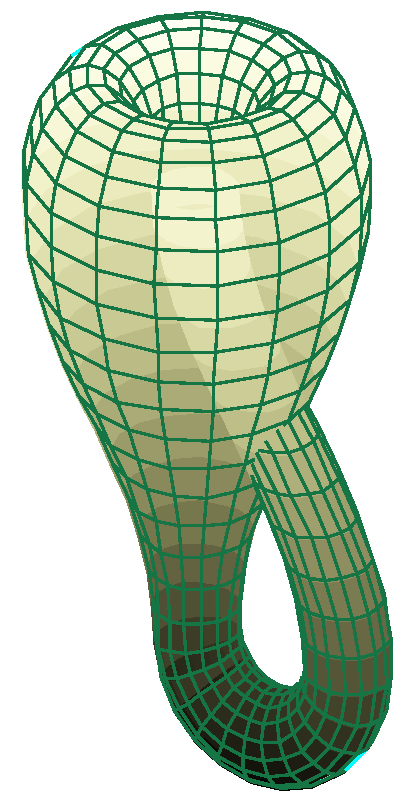
\includegraphics[height=4cm, keepaspectratio]{Bilder/Klein_bottle.pdf}
		\caption{Kleinsche Flasche, \href{https://en.wikipedia.org/wiki/File:Klein_bottle.svg}{Quelle}}
		}
	\end{figure}
	Übung: $K \cong T_{\substack{S^1 \to S^1 \\ z \mapsto -z}}$ 
\end{enumerate}
% subsection 12.3 (end)

\subsection[Satz: Zusammenhang der Fundamentalgruppe mit einer edk-Wirkung]{Satz} % (fold)
\label{sub:12.4}
Sei $X$ wegzusammenhängend und einfach zusammenhängend. Sei $G \wirkung X$ eine e.d.k. Wirkung. Für jedes $\overline{x}_0 \in G \backslash X$ ist dann 
\[
	\pi_1 \enbrace*{ G \backslash X, \overline{x}_0 } \cong G. 
\]
\minisec{Beweis}
Sei $x_0 \in X$ ein Urbild von $\overline{x}_0$, also $\overline{x}_0 = G \cdot x_0 $. Zu jeder Schleife $\omega : [0,1] \to G \backslash X$ mit 
$\omega(0) = \omega(1) = \overline{x}_0 $ gibt es eine Hebung $\hat{\omega} : [0,1] \to X$ mit $\hat{\omega}(0) = x_0$. Hier heben wir bezüglich der Überlagerung $p : X \to G \backslash X$, $x \mapsto G x$, also $p \circ  \hat{\omega} = \omega$.

Da $p \enbrace*{ \hat{\omega}(1)} = \omega(1) = \overline{x}_0 $ folgt $\omega(1)\in p ^{-1} (\overline{x}_0 ) = G \cdot x_0$.  Es gibt also $g_\omega \in G$ mit 
$g_\omega \cdot x_0 = \hat{\omega}(1)$. Wie im Fall der Überlagerung $\mathds{R} \to S^1$ zeigt man mit Hilfe des Homotopiehebungssatzes, dass $[\omega] \mapsto g_\omega$
ein Gruppenhomomorphismus $\varphi : \pi_1(G \backslash X, \overline{x}_0 ) \to G$ definiert. 
\begin{description}
	\item[Surjektivität von $\varphi$ :] Sei $g \in G$. Sei $\hat{\omega} : [0,1] \to X$ ein Weg von $x_0$ nach $g \cdot x_0$ (Solch ein Weg gibt es, da $X$ 
	wegzusammenhängend ist). Dann ist $\hat{\omega}$ die Hebung von $\omega := p \circ  \hat{\omega}$ und es folgt $\varphi( [\omega]) = g_\omega = g$, da 
	$\hat{\omega}(1) = g \cdot  x_0$. Also $g \in \im \varphi$.
	\item[Injektivität von $\varphi$ :] Sei $\omega : [0,1] \to G \backslash X$ eine Schleife und $\omega(0)= \omega(1) = x_0$ für die $\varphi([\omega]) = e$. Sei
	$\hat{\omega} : [0,1] \to X$ die Hebung von $\omega$ mit $\hat{\omega}(0) = x_0$. Da $\varphi([\omega]) = e$ gilt $\hat{\omega}(1) = x_0$, $\hat{\omega}$ ist also
	eine Schleife in $X$. Da $X$ einfach zusammenhängend ist, ist $[\hat{\omega}] = e \in \pi_1(X,x_0)$. Es folgt 
	\[
		[\omega] = [p \circ  \hat{\omega}] = p_* [\hat{\omega}] = p_*(e) = e. \bewende
	\]
\end{description}
% subsection 12.4 (end)

\subsection[Bemerkung: $S^n$ ist wegzusammenhängend, für $n \ge 2$ sogar einfach]{Bemerkung} % (fold)
\label{sub:12.5}
Für $n \ge 1$ ist $S^n$ wegzusammenhängend. \hfill  (einfache Übung) \\
Für $n \ge 2$ ist $S^n$ einfach zusammenhängend. \hfill (weniger einfache Übung) \medskip \\
Nach Satz \ref{sub:12.4} ist daher $\pi_1(\mathds{R}P^n, x_0) = \nicefrac{\mathds{Z}}{2}$ für $n \ge 2$. Es folgt $\mathds{R}P^n \not\cong S^n$ für $n \ge 2$. 
(Andererseits ist $\mathds{R}P^1 \cong S^1$.)
% subsection 12.5 (end)

\subsection[Definition: Decktransformation]{Definition} % (fold)
\label{sub:12.6}
Sei $p : \hat{X} \to X$ eine Überlagerung. Eine \Index{Decktransformation} von $p$ ist ein Homöomorphismus $f : \hat{X} \to \hat{X}$, sodass $p \circ f = p$. Die 
Decktransformationen von $p$ bilden eine Gruppe $\Delta(p)$. Diese Gruppe wirkt in kanonischer Wiese auf $\hat{X}$.
% subsection 12.6 (end)

\subsection{Lemma} % (fold)
\label{sub:12.7}
Sei $p : \hat{X} \to X$ eine Überdeckung wobei $\hat{X}$ wegzusammenhängend ist. Dann ist die Wirkung der Decktransformationsgruppe $\Delta(p)$ auf $\hat{X}$ eigentlich
diskontinuierlich.
\minisec{Beweis}
Wir zeigen zunächst, dass die Wirkung frei ist. Sei $f \in \Delta(p)$ und $x \in \hat{X}$ mit $f(x) = x$. Zu zeigen: $f =\id_{\hat{X}}$.
Sei $y \in \hat{X}$ und $\hat{\omega} : [0,1] \to \hat{X}$ ein
Weg von $x$ nach $y$. Dann sind $\hat{\omega}$ und $f \circ \hat{\omega}$ zwei Hebungen von $\omega := p \circ \hat{\omega}$. Da 
$\hat{\omega}(0) = x = f(x) = f \circ \hat{\omega}(0)$ folgt mit der Eindeutigkeit im Homotopiehebungssatz $\hat{\omega} = f \circ \hat{\omega}$ und insbesondere $y=f(y)$.
Da $y$ beliebig war, ist $f= \id_{\hat{X}}$.

Wir können nun zeigen, dass die Wirkung eigentlich diskontinuierlich ist: Sei $x \in \hat{X}$. Sei $U$ eine elementare Umgebung von $p(x)$. Dann ist $p ^{-1}(U)$ die 
disjunkte Vereinigung von offenen Mengen $V$, $V \in \mathcal{V}$ von denen jede homöomorph auf $U$ abgebildet wird. Sei $V_0 \in \mathcal{V}$ mit $x \in V_0$. Sei 
$f \in \Delta(p)$, $f \not= \id$. Für $y \in V_0$ gilt dann $p \enbrace*{f(y)} = p(y) $, $f(y) \not=y$ folgt $f(y) \not\in V_0$. Andernfalls wäre $p\big|_{V_0}$ nicht
injektiv. Daher $f(V_0) \cap V_0 = \emptyset$. \bewende
% subsection 12.7 (end)

\subsection{Bemerkung} % (fold)
\label{sub:12.8}
\begin{wrapfigure}{R}{3cm}
	\begin{tikzcd}
		\hat{X} \rar{p} \dar{q}& X \\
		H \backslash \hat{X} \urar[swap]{q'}&
	\end{tikzcd}
\end{wrapfigure}
Sei $p : \hat{X} \to X$ eine Überlagerung wobei $\hat{X}$ wegzusammenhängend ist. Sei $H \le \Delta(p)$ eine Untergruppe. Dann ist auch die Wirkung $H \wirkung \hat{X}$
eigentlich diskontinuierlich und die Quotientenabbildung $q : \hat{X} \to H \backslash \hat{X}$ eine Überlagerung. Weiter ist $q' : H \backslash \hat{X} \to X$ mit
$q'(Hx) := p(x)$ stetig, da $q' \circ q = p$ stetig ist. Ist $U \subseteq X$ elementar für $p$, so ist $U$ auch elementar für $q'$. $q'$ ist also auch eine Überlagerung.
Insgesamt haben wir also jeder Untergruppe von $\Delta (p)$ eine Überlagerung $H \backslash \hat{X}$ zugeordnet, die zwischen $\hat{X}$ und $X$ liegt.
% subsection 12.8 (end)

\subsection[Definition: Normale Überlagerung]{Definition} % (fold)
\label{sub:12.9}
Sei $p : \hat{X} \to X$ eine Überlagerung. Für $x \in X$ wirkt dann $\Delta(p)$ auf $p^{-1}(x)$. Die Überlagerung heißt 
\bet{normal}\index{Überlagerung!normal}, falls diese Wirkung transitiv ist, d.h. falls es zu $\hat{x}, \hat{y} \in p^{-1}(x)$ immer $f \in \Delta(p)$ gibt mit 
$f(\hat{x})= \hat{y}$.
% subsection 12.9 (end)

\subsection{Proposition} % (fold)
\label{sub:1210}
Sei $\hat{X} \xrightarrow{p} X $ eine normale Überlagerung wobei $\hat{X}$ wegzusammenhängend ist. Dann ist die Abbildung $q' : \Delta(p)\backslash \hat{X} \to X$,
$q' \enbrace*{\Delta(p) x} = p(x)$ ein Homöomorphismus. \\
Wenn zusätzlich $\hat{X}$ einfach zusammenhängend und wegzusammenhängend ist, dann gilt $\pi_1(X, x_0) \cong \Delta(p)$ für einen beliebigen Basispunkt $x_0 \in X$.
\minisec{Beweis}
Wir haben schon gesehen, dass $q'$ eine Überlagerung ist. Unabhängig davon ob $p$ normal ist. Ist $p$ normal, so ist $q'$ bijektive Überlagerung und daher Homöomorphismus.
\bewende 
% subsection 1210 (end)
% section 12 (end)
\newpage

\section{Klassifikation von Überlagerungen} % (fold)
\label{sec:13}

\subsection{Hebungssatz} % (fold)
\label{sub:131}
Sei $p: \hat{X} \to X$ eine Überlagerung. Sei $x_0 \in X, \hat{x}_0 \in \hat{X}$, $p(\hat{x}_0)= x_0$. Sei $Z$ wegzusammenhängend und lokal wegzusammenhängend. Sei 
$z_0 \in Z$, $f : Z \to X$ stetig mit $f(z_0)= x_0$. Dann gibt es eine Hebung $\hat{f} : Z \to \hat{X}$ mit $\hat{f} (z_0) = \hat{x}_0$ genau dann, wenn 
\[
	f_*\enbrace[\big]{\pi_1 (Z, z_0)} \subseteq  p_* \enbrace[\big]{\pi_1(\hat{X}, \hat{x}_0)} \tag*{$(\star)$}
\]
als Untergruppe von $\pi_1(X,x_0)$ gilt. In diesem Fall ist $\hat{f}$ eindeutig.
\[
	\begin{tikzcd}
		X & \hat{X} \lar[swap]{p} \\
		Z \uar{f}  \urar[dashed, swap]{\hat{f}}&
	\end{tikzcd}
\]
\minisec{Beweis}
Existiert $\hat{f}$, so folgt $(\star)$ aus $f_* = p_* \circ\hat{f}_*$. Sei umgekehrt $(\star)$ erfüllt. Sei $z\in Z$. Sei $\omega : [0,1]\to Z$ ein Weg von $z_0$ nach $z$.
Sei $\hat{\omega} : [0,1] \to \hat{X}$ die eindeutige Hebung von $f \circ \omega$ mit $\hat{\omega}(0)= \hat{x}_0$ (Homotopiehebungssatz, \ref{sub:108}). Existiert 
$\hat{f}$ so ist auch $\hat{f} \circ \omega$ eine Hebung von $f \circ \omega$ mit $\hat{f} \circ \omega (0) = \hat{f}(z_0)= \hat{x}_0$, also 
$\hat{\omega} = \hat{f} \circ \omega$ und insbesondere ist $\hat{f}(z)= \hat{f} \enbrace[\big]{\omega(1)} = \hat{\omega}(1)$. Daher ist $\hat{f}$ eindeutig, falls es 
existiert.

Zur Existenz setzen wir $\hat{f}(z) := \hat{\omega}(1)$. Wir müssen zeigen:
\begin{description}
	\item[Wohldefiniertheit:] Sei $\eta : [0,1] \to Z$ ein zweiter Weg von $z_0$ nach $z$. Sei $\hat{\eta} : [0,1] \to \hat{X}$ die zugehörige Hebung. Zu zeigen: 
	$\hat{\eta}(1) = \hat{\omega}(1)$. Betrachte die Schleife $\overline{\omega} * \eta$ in $Z$. Dann ist $\overline{\hat{\omega}} * \hat{\eta}$ eine Hebung von
	$f \circ (\overline{\omega} * \eta)$. Aus $(\star)$ folgt, dass $f \circ (\overline{\omega} * \eta )$ im Bild von $p_* : \pi_1(\hat{X}, \hat{x}_0) \to \pi_1(X,x_0)$ 
	liegt. Mit dem Homotopiehebungssatz ergibt sich, dass auch $\overline{\hat{\omega}} * \hat{\eta}$ eine Schleife ist (Übung!). Damit folgt 
	$\hat{\omega}(1)= \hat{\eta}(1)$
	\item[Stetigkeit:] Sei $U \subseteq \hat{X}$ offen. Sei $z \in \hat{f} ^{-1} (U)$. Sei $V$ eine elementare Umgebung von $f(z)$. Indem wir $V$ wenn nötig klein machen
	erhalten wir eine offene Umgebung $V'$ von $\hat{f}(z)$, die unter $p$ homöomorph auf $V$ abgebildet wird. Da $f$ stetig ist und $Z$ lokal wegzusammenhängend ist, gibt
	es eine wegzusammenhängende Umgebung $W$ von $z$ mit $f(W) \subseteq V$. Sei nun $\omega : [0,1] \to Z$ ein Weg von $z_0$ nach $z$. Zu $z' \in W$ gibt es einen Weg
	$\eta : [0,1] \to W$ von $z$ nach $z'$ und $\omega * \eta$ ist ein Weg von $z_0$ nach $z'$. Insbesondere ist 
	\[
		\hat{f}(z') = \widehat{(\omega * \eta)} (1)= \hat{\omega} * p\big|_{V'} ^{-1} (\eta) (1) = \enbrace*{p \big|_{V'}} ^{-1} \enbrace[\big]{\eta(1)} \in V'  
	\]
	Also $\hat{f}(W) \subseteq V' \subseteq U$. \bewende
\end{description}
% subsection 131 (end)

\subsection{Klassifikationssatz (Eindeutigkeit)} % (fold)
\label{sub:132}
Seien $p_1 : \hat{X}_1 \to X$, $p_2 : \hat{X}_2 \to X$ zwei Überlagerungen. Dabei seien $\hat{X}_1$ und $\hat{X}_2$ wegzusammenhängend und lokal wegzusammenhängend.
Seien $\hat{x}_1 \in \hat{X}_1$, $\hat{x}_2 \in \hat{X}_2$ mit $p_1(\hat{x}_1) = x_0 = p_2(\hat{x}_2)$.
Dann sind äquivalent:
\begin{enumerate}[a)]
	\item Es gibt einen Homöomorphismus $f : \hat{X}_1 \to \hat{X}_2$ mit $p_2 \circ f = p_1$ und $f(\hat{x}_1) = \hat{x}_2$.
	\item ${p_1}_*\enbrace*{\pi_1 \enbrace*{\hat{X}_1, \hat{x}_1}} = {p_2}_* \enbrace*{\pi_1 \enbrace*{\hat{X}_2, \hat{x}_2}}$ als Untergruppen von $\pi_1(X,x_0)$
\end{enumerate}
\minisec{Beweis}
\begin{description}
	\item[a) $\Rightarrow$ b):] Ist $f$ wie in a), so ist $f_* : \pi_1 \enbrace*{\hat{X}_1, \hat{x}_1} \to \pi_1 \enbrace*{\hat{X}_2, \hat{x}_2}$ ein Isomorphismus und es 
	folgt 
	\[
		(p_1)_* \enbrace*{\pi_1 \enbrace*{\hat{X}_1, \hat{x}_1}} =  (p_2 \circ f)_* \enbrace*{\pi_1 \enbrace*{\hat{X}_1, \hat{x}_1}} 
		= (p_2)_* \circ (f)_* \enbrace*{\pi_1 \enbrace*{\hat{X}_1, \hat{x}_1}} = (p_2)_* \enbrace*{\pi_1 \enbrace*{\hat{X}_2, \hat{x}_2}}
	\]
	\item[b) $\Rightarrow$ a):] Betrachte
	\[
		\begin{tikzcd}
			\mbox{ } & \hat{X}_2 \dar{p_2}\\
			\hat{X}_1 \rar{p_1} \urar[dashed]{f}& X
		\end{tikzcd}
	\]
	Hebungssatz $\Rightarrow \exists$ $f : \hat{X}_1 \to \hat{X}_2$ mit $p_2 \circ f = p_1$, $f(\hat{x}_1) = \hat{x}_2$. Weiter ist
	\[
		\begin{tikzcd}
			\mbox{} & \hat{X}_1\dar{p_1} \\
			\hat{X}_2 \rar{p_2} \urar[dashed]{g}&  X
		\end{tikzcd}
	\]
	Wieder liefert der Hebungssatz: $\exists \, g : \hat{X}_2 \to \hat{X}_1$ mit $p_1 \circ  g = p_2$, $g(\hat{x}_2) = \hat{x}_1$. Betrachte nun
	\[
		\begin{tikzcd}[column sep=4em, row sep=4em]
			\mbox{ } & \hat{X}_1 \dar{p_1}\\
			\hat{X}_1 \rar{p_1} \urar[swap]{\id_{\hat{X}_1}} \urar[bend left]{g \circ f} & X
		\end{tikzcd}
	\]
	Die Eindeutigkeit im Hebungssatz liefert $g \circ f = \id_{\hat{X}_1}$. Analog folgt $f \circ g = \id_{\hat{X}_2}$ \bewende.
\end{description}
% subsection 132 (end)

\subsection{Satz (Universelle Überlagerung)} % (fold)
\label{sub:133}
Sei $X$ wegzusammenhängend, lokal wegzusammenhängend und lokal einfach zusammenhängend. Dann gibt es eine wegzusammenhängende und einfach zusammenhängende  Überlagerung 
$\tilde{X} \xrightarrow{p} X $
\minisec{Konstruktionsskizze}
Sei $x_0 \in X$. Sei $P = \set[{\omega : [0,1] \to X \text{ Weg}}]{\omega(0)=x_0} $. Sei $\tilde{X}:= \nicefrac{P}{\text{Homotopie mit festen Endpunkten}}$. Dann induziert
$\omega \mapsto \omega(1)$ eine wohldefinierte Abbildung $p : \tilde{X} \to X$. Sei $\omega \in P$ und $V$ eine wegzusammenhängende einfach zusammenhängende Umgebung
von $\omega(1)$ in $X$. Setze 
\[
	U(V,\omega) = \set[{[\omega * \eta]}]{\rule{0cm}{1em} \eta : [0,1] \to V \text{ Weg mit } \eta(0)= \omega(1)} 
\]
Die $U(V,\omega)$ bilden die Basis der Topologie von $\tilde{X}$. Da $V$ wegzusammenhängend und einfach zusammenhängend ist, ist 
\[
	p \Big|_{U(V,\omega)} : U(V,\omega) \to V
\]
bijektiv. Da $X$ lokal wegzusammenhängend und lokal einfach zusammenhängend ist, ist $p \big|_{U(V,\omega)}$ sogar ein Homöomorphismus. Damit ist $V$ eine elementare 
Umgebung von $\omega(1)$. Da $X$ wegzusammenhängend ist, ist $p$ auch surjektiv und $p : \tilde{X} \to X$ eine Überlagerung.

\uline{$\tilde{X}$ ist wegzusammenhängend:} Sei $\tilde{x}_0 := [c_{x_0}] \in \tilde{X}$. Sei $\tilde{x} = [\omega] \in \tilde{X}$. Sei $\omega_s : [0,1] \to X$ mit
\[
	\omega_s(t) = \begin{cases}
		\omega(t), &\text{ falls }t \le s\\
		\omega(s), &\text{ falls } t  \ge s
	\end{cases}
\]
Dann ist $\alpha : [0,1] \to \tilde{X}$ mit $\alpha(s) = [\omega_s]$ ein Weg von $\tilde{x}_0$ nach $\tilde{x}$.
% subsection 133 (end)

\subsection[Definition; Universelle Überlagerung]{Definition} % (fold)
\label{sub:134}
$\tilde{X} \xrightarrow{p} X $ heißt die \bet{universelle Überlagerung}\index{Überlagerung!universell} von $X$.
% subsection 134 (end)

\subsection{Klassifikationssatz (Existenz)} % (fold)
\label{sub:135}
Sei $X$ wegzusammenhängend, lokal wegzusammenhängend und lokal einfach zusammenhängend. Sei $x_0 \in X$. Dann gibt es zu jeder Untergruppe $H \le \pi_1(X,x_0)$ eine
Überlagerung $q : \hat{X} \to X$ und $\hat{x}_0 \in p ^{-1} (x_0)$ mit $q_* \enbrace*{\pi_1(\hat{X}, \hat{x}_0)} = H $
\minisec{Beweis}
Sei $p : \tilde{X} \to X$ die universelle Überlagerung. Der Hebungssatz impliziert, dass $p : \tilde{X} \to X$ normal ist. Es folgt $\Delta(p) \backslash \tilde{X} \cong X$
und $\pi_1(X, x_0) \simeq \Delta(p)$. Genauer: Zu $\tilde{x}_0 \in p ^{-1}(x_0)$ gibt es einen Isomorphismus $\varphi : \Delta (p) \to \pi_1(X,x_0)$ mit 
\[
	\varphi(f) = [p \circ \tilde{\omega}_f]
\]
wobei $\tilde{\omega} : [0,1] \to \tilde{X}$ ein Weg von $\tilde{x}_0$ nach $f (\tilde{x}_0)$ ist. Setze $H_\Delta := \varphi ^{-1}(H)  \le \Delta(p)$. Wir erhalten
Überlagerungen $\tilde{X} \xrightarrow{q'} H_\Delta \backslash \tilde{X} \xrightarrow{q} X $ mit $q'(x) = H_\Delta x$, $q (H_\Delta x) = p(x)$. Da $\tilde{X}$ einfach
zusammenhängend ist, ist $\pi_1 \enbrace*{ H_\Delta \backslash \tilde{X}, H_\Delta \hat{x}_0} \cong H_\Delta$. Sei $\hat{x}_0 := H_\Delta \tilde{x}_0$.
Genauer gibt es einen Isomorphismus $\psi : H_\Delta \to \pi_1 \enbrace*{H_\Delta \backslash \tilde{X}, \hat{x}_0}$ mit
\[
	\psi(f) = [q' \circ  \omega_f]
\]
Es folgt 
\[
	q_* \enbrace*{\psi(f)} = q_* [q' \circ \omega_f] = [q \circ q' \circ \omega_f] = [p \circ \omega_f] = \psi(f) 
\]
Also $q_* \enbrace*{\pi_1 \enbrace*{H_\Delta \backslash \tilde{X}, \hat{x}_0}} = H $. \bewende
% subsection 135 (end)
% section 13 (end)
\newpage

\section{Höhere Homotopiegruppen} % (fold)
\label{sec:14}
\emph{Dieses Kapitel ist nur ein kleiner Exkurs zu einem Thema, das auch ganze Vorlesungsreihen füllen könnte.}
\subsection{Rückblick} % (fold)
\label{sub:141}
Sei $(X,x_0)$ ein punktierter Raum. Sei in diesem Abschnitt $I= [0,1]$. Wegzusammenhängend: Punkte in $X \hat{=} I^0 = \set{x} \to X$. Wege in $X$ sind dann Homotopien 
solcher Abbildungen. $\pi_0(X,x_0) $ ist dann die (punktierte) Menge der Homotopieklassen von Abbildungen $I^0 \to X$. Die Schleifen in $X$ sind
stetige Abbildungen $\omega : I\to X$ mit $\omega(0)= x_0 = \omega(1)$. $\pi_1(X,x_0)$ ist die Menge der Homotopieklassen von Schleifen und heißt die Fundamentalgruppe.
% subsection 141 (end)

\subsection[Definition: Homotopie von für Abbildungen $I^n \to X$]{Definition} % (fold)
\label{sub:142}
Seien $\omega_0, \omega_1 : I^n \to X$ stetige Abbildungen mit $\omega_0(\partial I^n)= \set{x_0} = \omega_1(\partial I^n)$. Eine \Index{Homotopie} zwischen $\omega_0$ und
$\omega_1$ ist eine stetige Abbildung $H : I^n \times [0,1] \to X$, sodass Folgendes gilt:
\begin{itemize}
	\item $H(s_1, \ldots , s_n, 0) = \omega_0(s_1, \ldots , s_n)$ für alle $(s_1, \ldots , s_n) \in I^n$
	\item $H(s_1, \ldots , s_n, 1) = \omega_1(s_1, \ldots , s_n)$ für alle $(s_1, \ldots , s_n) \in I^n$
	\item $H(s_1, \ldots , s_n, t) = x_0$ für alle $t \in [0,1]$, $(s_1, \ldots , s_n) \in \partial I^n$
\end{itemize}
\minisec{Bemerkung}
Homotopie ist eine Äquivalenzrelation.
% subsection 142 (end)

\subsection[Definition: Höhere Homotopiegruppe]{Definition} % (fold)
\label{sub:143}
Sei $(X,x_0)$ ein punktierter Raum. Definiere $\pi_n(X,x_0)$ also die Menge der Homotopieklassen von Abbildungen $\omega : I^n \to X$ mit $\omega(\partial I^n)=\set{x_0} $
\marginnote{für $n>0$}.
\minisec{Bemerkung}
Für $n=2$ \marginnote{Rand auf einen Punkt kollabieren}
\[
	\begin{tikzcd}
		I^2 \rar["\omega"] \arrow[d, two heads]& X \\
		\nicefrac{I^2}{\partial I^2} \urar[dashed, "\exists"]
	\end{tikzcd} \qquad \qquad 
	\vcenter{\hbox{\begin{tikzpicture}
		\draw (0,0) rectangle (2,2);
	\end{tikzpicture}}}
	\enspace\twoheadrightarrow \enspace
	\vcenter{\hbox{
	\begin{tikzpicture}
		\draw (-1,0) arc (180:360:1cm and 0.5cm);
	    \draw[dashed] (-1,0) arc (180:0:1cm and 0.5cm);
	    \draw (0,1) arc (90:270:0.5cm and 1cm);
	    \draw[dashed] (0,1) arc (90:-90:0.5cm and 1cm);
	    \draw (0,0) circle (1cm);
	    \shade[ball color=blue!10!white,opacity=0.20] (0,0) circle (1cm);
	\end{tikzpicture}}}
\]
allgemein: Abbildung $\omega : I^n \to X$ mit $\omega(\partial I^n) = \set{x_0}$ $\leadsto$ punktierte Abbildung $(S^n, s_0) \to (X,x_0)$.
% subsection 143 (end)

\subsection{Definition} % (fold)
\label{sub:144}
Sei $1 \le k \le n$, $\omega_0, \omega_1 : I^n \to X$, $\omega_i(\partial I^n) = \set{x_0}$ für $i=1,2$. Definiere:
\[
	\enbrace*{\omega *_k \omega'} (s_1, \ldots , s_n) := \begin{cases}
		\omega(s_1, \ldots , s_{k-1}, 2 s_k, s_{k+1}, \ldots , s_n), &\text{ falls } 0 \le s_k, \le \frac{1}{2} \\
		\omega(s_1, \ldots , s_{k-1}, 1- 2 s_k, s_{k+1}, \ldots , s_n), &\text{ falls } \frac{1}{2} \le s_k \le 1 
	\end{cases} 
\]
% subsection 144 (end)

\subsection{Lemma (Eckmann-Hilton-Arguemnt)} % (fold)
\label{sub:145}
Sei $A$ eine Menge mit zwei inneren Verknüpfungen $\boxempty, \diamond : A \times A\to A $, sodass gilt:
\begin{enumerate}[a)]
	\item Es gibt $e \in A$ mit $e \boxempty a = a \boxempty e = a = e \diamond a = a \diamond e$ für alle $a \in A$
	\item Für alle $a,b,c,d \in A$ gilt $(a \boxempty b) \diamond (c \boxempty d) = (a \diamond c) \boxempty (b \diamond d)$.
\end{enumerate}
Dann stimmen $\boxempty$ und $\diamond $ überein, sind assoziativ und kommutativ.
\minisec{Beweis}
\begin{align*}
	a \boxempty b &= (e \diamond a) \boxempty (b \diamond e) = (e \boxempty b) \diamond (a \boxempty e) = b \diamond a \\
	b \diamond a &= (b \boxempty e) \diamond (e \boxempty a) = (b \diamond e) \boxempty (e \diamond a) = b \boxempty a
\end{align*}
$\Rightarrow \boxempty = \diamond$ und ist kommutativ + Assoziativität. \bewende
% subsection 145 (end)

\subsection{Proposition} % (fold)
\label{sub:146}
\begin{enumerate}[a)]
	\item $1 \le k \le n$, $\omega_0, \omega_0', \omega_1, \omega_1' : I^n \to X$ stetig mit $\omega_i (\partial I^n) = \set{x_0} = \omega_i'(\partial I^n)$ für $i=0,1$.
	Es gelte $[\omega_0] = [\omega_1]$, $[\omega_0'] = [\omega_1']$ in $\pi_n(X,x_0)$. Dann gilt 
	\[
		[\omega_0 *_k \omega_0'] = [\omega_1 *_k \omega_1'] \in \pi_n(X, x_0)
	\]
	Schreibe $\cdot_k$ für die induzierte Verknüpfung.
	\item $1 \le k,l \le n$. Dann gilt $\cdot_k = \cdot_l$. Für $n \ge 2$ ist $\cdot $ kommutativ. Außerdem assoziativ.
	\item $\pi_n(X,x_0)$ ist eine abelsche Gruppe für $n \ge 2$.
	\item $f : (X,x_0) \to (Y,y_0)$ stetig. Dann definiert $[\omega] \mapsto [f \circ \omega]$ einen Gruppenhomomorphismus $\pi_n(f) : \pi_n(X,x_0) \to \pi_n(Y,y_0)$,
	falls $n \ge 1$.
	\item $\pi_n(\id_X) = \id_{\pi_n(X,x_0)}$, $\pi_n(f \circ g) = \pi_n(f) \circ \pi_n(g)$
	\item Ist $f$ punktiert homotop zu $g$, so gilt $\pi_n(f) = \pi_n(g)$.
\end{enumerate}
\minisec{Zum Beweis}
\begin{enumerate}[a)]
	\item \checked
	\item für $n=2$
	\[
		\begin{array}{c}
			(\omega *_1 \omega') \\
			*_2 \\
			(\omega'' *_1 \omega''')
			
		\end{array}
		 = 
		\vcenter{\hbox{\begin{tikzpicture}
			\draw (0,0) grid (2,2);
			\node at (0.5,0.5){$\omega''$};
			\node at (0.5,1.5){$\omega$};
			\node at (1.5,0.5){$\omega'''$};
			\node at (1.5,1.5){$\omega'$};
		\end{tikzpicture}}}
		 = \begin{pmatrix}
		 	\omega \\
			*_2 \\
			\omega''
		 \end{pmatrix} *_1
		 \begin{pmatrix}
		 	\omega' \\
			*_2 \\
			\omega'''
		 \end{pmatrix}
	\]
	Mit Eckmann-Hilton-Argument folgt $\cdot_k = \cdot_l$ und für $n \ge 2 $ kommutativ.
	\item Gegeben $\omega : I^n \to X$, definiere $\overline{\omega} (s_1, \ldots , s_n) := \omega (1-s_1, s_2, \ldots , s_n)$. Damit ist $[\overline{\omega}]$ Inverses von
	$[\omega]$
	\item einfach
	\item einfach
	\item einfach \bewende
\end{enumerate}
% subsection 146 (end)

\subsection{Korollar} % (fold)
\label{sub:147}
$(X,x_0) \sim (Y,y_0) \Rightarrow \pi_n(X,x_0) \cong \pi_n(Y,y_0)$ für alle $n$. Insbesondere: $(X,x_0)$ zusammenziehbar $\Rightarrow \pi_n(X,x_0) = 0$ für $n \ge 2$.
% subsection 147 (end)

\subsection{Proposition} % (fold)
\label{sub:148}
$p : \hat{X} \to X$ Überlagerung. $\hat{x}_0 \in \hat{X}, x_0 \in X$ mit $p(\hat{x}_0) = x_0$. Dann ist $\pi_n(p) : \pi_n(\hat{X}, \hat{x}_0) \to \pi_n(X,x_0)$ ein
Isomorphismus für $n \ge 2$
\minisec{Beweis}
Übung.
% subsection 148 (end)

\subsection{Korollar} % (fold)
\label{sub:149}
$\pi_n(S^1, s_0) = 0$ für $n \ge 2$
\minisec{Beweis}
Es gibt eine Überlagerung $R \to S^1$. \bewende
% subsection 149 (end)

\subsection[Definition: Faserung]{Definition} % (fold)
\label{sub:1410}
Eine stetige Abbildung $p : E \to B$ heißt (Serre-)\Index{Faserung}, falls sie folgende Homotopiehebungseigenschaft hat: Für jedes $n \ge 0$, jede Homotopie 
$H : I^n \times [0,1] \to B$ und jede partielle Hebung $\tilde{H} : I^n \times \set{0} \cup \partial I^n \times [0,1]$ existiert eine Hebung $\overline{H}$ von $H$
entlang $p$, die $\tilde{H}$ fortsetzt. Nenne $p ^{-1}(b)$ die \Index{Faser} über $b$. 
\[
	\begin{tikzcd}
		I^n \times \set{0} \cup \partial I^n \times [0,1] \rar["\tilde{H}"]  \dar[hook]& E \dar["p"] \\
		I^n \times [0,1] \rar \urar[dashed, "\overline{H} "]& B
	\end{tikzcd}
\]
\minisec{Beispiel}
\begin{itemize}
	\item Überlagerungen sind Faserungen (!)
	\item Die Projektion $B \times F \to B$ ist eine Faserung.
\end{itemize}
% subsection 1410 (end)

\subsection{Satz} % (fold)
\label{sub:1411}
Sei $p : E \to B$ eine Faserung. Seien $b_0 \in B, e_0 \in E$ mit $p(e_0)= b_0$. Setze $F := p ^{-1}(b)$. Sei $i : (F, e_0) \hookrightarrow (E,e_0)$ die Inklusion.
Dann existiert eine lange exakte Sequenz
\begin{align*}
	\ldots  \pi_{n+1}(B,b_0) &\xrightarrow{\partial_{n+1}} \pi_n(F,e_0) \xrightarrow{\pi_n(i)} \pi_n(E,e_0) \xrightarrow{\pi_n(p)} \pi_n(B,b_0)  \xrightarrow{\partial_n} 
	\pi_{n-1}(F,e_0) \ldots \\
	&\longrightarrow \pi_1(B,b_0) \xrightarrow{\partial_1} \pi_0(F,e_0) \xrightarrow{\pi_0(i)} \pi_0(E,e_0) \xrightarrow{\pi_0(p)} \pi_0(B,b_0)   
\end{align*}
D.h.
\begin{itemize}
	\item $\partial_n$ ist ein Homomorphismus für $n >2$.
	\item $\ker \pi_n(p) = \im \pi_n(i)$, $\ker( \partial_{n+1}) = \im \pi_{n+1}(p)$, $\ker \pi_n(i) = \im \partial_{n+1}$ für $n \ge 1$
	\item $\partial_1(x) = [e_0] \iff x \in \im \pi_n(p)$
	\item $\pi_0(i)(x) = [e_0] \iff x \in \im \partial_1$
	\item $\pi_0(p)(x) = [b_0] \iff x \in \im \pi_0 (i)$
\end{itemize}
\minisec{Zum Beweis}
Definition von $\partial_n$: Sei $\omega : I^n \to B, \omega(\partial I^n) = \set{b_0} $.
\[
	\begin{tikzcd}
		I^{n-1} \times \set{0} \cup \partial I^{n-1} \times [0,1] \rar["\mathrm{const}_{e_0}"] \dar[hook]& E \dar["p"] \\
		I^{n-1} \times [0,1] \rar["\omega"] \urar[dashed, "\tilde{\omega}"]& B 
	\end{tikzcd}
\]
$\tilde{\omega}\Big|_{I^{n-1} \times \set{1}} : I^{n-1} \to F$, konstant auf $\partial I^{n-1}$. Definiere 
$\partial_n([\omega]) := \benbrace*{\tilde{\omega}\Big|_{I^{n-1} \times \set{1}}} $. $\partial_n$ ist wohldefiniert und Homomorphismus für $n >2$.
% subsection 1411 (end)

\subsection{Anwendung} % (fold)
\label{sub:1412}
Es gibt eine Faserung $S^3 \xrightarrow{p} S^2 $, sodass $p ^{-1}(s) \cong S^1$ (\enquote{Hopf-Faserung}). Es gilt $\pi_1(S^n)= 1$ für $n \ge 2$, $\pi_2(S^3)= 0$
Betrachte:
\begin{align*}
	\ldots  &\longrightarrow \underbrace{\pi_3(S^1)}_{=0} \longrightarrow \pi_3(S^3) \longrightarrow \pi_3(S^2) \longrightarrow \underbrace{\pi_2(S^1)}_{=0} \\
	&\longrightarrow \underbrace{\pi_2(S^3)}_{=0} \longrightarrow \pi_2(S^2) \longrightarrow \pi_1(S^1) \longrightarrow \underbrace{\pi_1(S^3)}_{=1} \longrightarrow \ldots 
\end{align*}
Mit Exaktheit folgt $\pi_2(S^2) \cong \pi_1(S^1) \cong \mathds{Z}$ und $\pi_3(S^3) \cong \pi_3(S^2)$. Tatsache: $\pi_3(S^3) \cong \mathds{Z}$.
% subsection 1412 (end)
% section 14 (end)
\newpage

\section{Differenzierbare Mannigfaltigkeiten} % (fold)
\label{sec:15}

\subsection[Frage zur Differenzierbarkeit von Funktionen auf Mannigfaltigkeiten]{Frage} % (fold)
\label{sub:151}
Sei $M$ eine topologische Mannigfaltigkeit. Welche Funktionen $f : M \to \mathds{R}$ sind differenzierbar? Was sind Richtungsableitungen für solche Funktionen? Was sind 
Richtungen in $M$?
\minisec{Ansatz}
$f : M \to \mathds{R}$ heißt $C^\infty :\Leftrightarrow \forall x \in M : \exists x \in U \subseteq M$, $h : U \xrightarrow{\cong}  V \subseteq \mathds{R}^n : f \circ h ^{-1} : V \to \mathds{R}$ ist $C^\infty$ \\
\textbf{Aber:}
\begin{enumerate}[a)]
	\item Ob $f \circ h ^{-1} : V \to R$ $C^\infty$ ist oder nicht, hängt von der Wahl von $h$ ab.
	\item Jeder Homöomorphismus $f : \mathds{R} \to \mathds{R}$ ist in dieser Definition $C^\infty$!
\end{enumerate}
% subsection 151 (end)

\subsection[Definition: Karten, Kartenwechsel, Atlanten]{Definition} % (fold)
\label{sub:152}
Sei $M^n$ eine topologische $n$-Mannigfaltigkeit. 
\begin{enumerate}[a)]
	\item Eine \Index{Karte} für $M$ ist ein Homöomorphismus $h : U \xrightarrow{\approx}V$ mit $U \subseteq M$ offen, $V\subseteq\mathds{R}^n$ offen. $U$ heißt das 
	\Index{Kartengebiet} von $h$. Ist $x \in U$, so heißt $h$ eine \bet{Karte um} $x$.
	\item Sind $h_i : U_i \xrightarrow{\approx} V_i$, $i=0,1$ zwei Karten, so heißt 
	\[
		h_1 \circ h_0 ^{-1}\big|_{h_0(U_0 \cap U_1)} : \underset{\subseteq V_0 \subseteq \mathds{R}^n}{h_0(U_0 \cap U_1)} \to \underset{\subseteq V_1 \subseteq 
		\mathds{R}^n}{h_1 (U_0 \cap U_1)}
	\]
	der \Index{Kartenwechsel} zwischen $h_0$ und $h_1$. Ein Kartenwechsel ist ein Homöomorphismus zwischen offenen Teilmengen des $\mathds{R}^n$. 
	\item Eine Menge von Karten $\set[h_\alpha : U_\alpha \to V_\alpha]{\alpha \in A}$ heißt ein \Index{Atlas} für $M$, wenn die Kartengebiete $U_\alpha$ die 
	Mannigfaltigkeit überdecken:
	\(
		M = \bigcup_{\alpha \in A} U_\alpha
	\)
	\item Ein Atlas $\mathcal{A}$ heißt $C^\infty$ (oder \bet{glatt}\index{Atlas!glatt}), wenn alle Kartenwechsel zwischen Karten aus $\mathcal{A}$ 
	$C^\infty$-Abbildun\-gen sind.
\end{enumerate}
% subsection 152 (end)

\subsection[Definition: Differenzierbare Mannigfaltigkeit]{Definition} % (fold)
\label{sub:153}
Eine $C^\infty$-Mannigfaltigkeit ist eine topologische Mannigfaltigkeit zusammen mit einem $C^\infty$-Atlas $\mathcal{A}$.
% subsection 153 (end)

\subsection[Beispiele für differenzierbare Mannigfaltigkeiten]{Beispiele} % (fold)
\label{sub:154}
\begin{enumerate}[(1)]
	\item $U \subseteq \mathds{R}^n$ offen ist eine $C^\infty$-Mannigfaltigkeit mit Atlas $\set{\id_U}$.
	\item $S^n$: Definiere Kartengebiete $U_{kj} := \set[x \in S^n]{(-1)^j x_k > 0}$ für $k=0, \ldots, n$, $j=0,1$. Sei 
	\[
		h_{kj} : U_{kj} \to \mathring{D}^n = \set[x \in \mathds{R}^n]{\norm[2]{x} < 1 } 
	\]
	mit 
	\[
		h_{kj} (x_0, \ldots , x_n) = (x_0, \ldots , x_{k-1}, x_{k+1}, \ldots , x_n)
	\]
	Dann ist $\mathcal{A} = \set[h_{kj}]{k=0, \ldots ,n \enspace j=0,1}$ ein $C^\infty$-Atlas für $S^n$.
	\item $\mathds{R}P^n = \nicefrac{S^n}{x \sim -x}$: Setze 
	\[
		U_k := \set[{\benbrace[\big]{(x_0, \ldots, x_n)} \in \mathds{R}P^n}]{x_k \not= 0} 
	\]
	und definiere $h_k : U_k \to \mathring{D}^n$ durch
	\[
		h_k \enbrace[\big]{[x_0, \ldots, x_n]} = \frac{x_k}{\abs*{x_k}} \enbrace*{x_0, \ldots , x_{k-1}, x_{k+1}, \ldots, x_n} .  
	\]
	Dann ist $\set[h_k]{k=0,\ldots , n}$ ein $C^\infty$-Atlas für $\mathds{R}P^n$.
	\item Sind $(M, \mathcal{A})$ und $(N, \mathcal{B})$ $C^\infty$-Mannigfaltigkeiten, so ist $\set[h \times k]{h \in \mathcal{A}, k \in \mathcal{B}}$ ein
	$C^\infty$-Atlas für $M \times N$.
\end{enumerate}
% subsection 154 (end)

\subsection[Bemerkung: Maximaler Atlas]{Bemerkung} % (fold)
\label{sub:155}
Sei $(M,\mathcal{A})$ eine $C^\infty$-Mannigfaltigkeit. Eine Karte $h : U \to V$ für $M$ (nicht notwendig in $\mathcal{A}$) heißt eine $C^\infty$-Karte, wenn alle 
Kartenwechsel zwischen $h$ und einer Karte aus $\mathcal{A}$ $C^\infty$ sind. Offenbar besteht $\mathcal{A}$ aus $C^\infty$-Karten. Es ist auch 
$\mathcal{A}_\mathrm{max} := \set[h]{h \text{ ist $C^\infty$-Karte}}$ ein $C^\infty$-Atlas für $M$. Dieser Atlas ist maximal, d.h. man kann keine weiteren Karten zu 
$\mathcal{A}_\mathrm{max}$ hinzufügen und immer noch einen $C^\infty$-Atlas erhalten.
% subsection 155 (end)

\subsection[Definition: Differenzierbarkeit einer Abbildung $f : M \to N$]{Definition} % (fold)
\label{sub:156}
Seien $M,N$ $C^\infty$-Mannigfaltigkeiten. Sei $f : M \to N$ eine stetige Abbildung.
\begin{enumerate}[a)]
	\item Sei $x \in M$. $f$ heißt $C^\infty$ oder \bet{glatt}\index{Differenzierbarkeit} in $x$, wenn es eine Karten $h_0 : U_0 \to V_0$ von $M$ um $x$ und 
	$h_1 : U_1 \to V_1$ von $N$ um $f(x)$ gibt, sodass 
	\[
		h_1 \circ f \circ h_0 ^{-1}
	\]
	auf einer Umgebung von $h_0(x)$ eine $C^\infty$-Abbildung ist.
	\item Ist $f$ in allen $x \in M$ glatt, so heißt $f$ eine \bet{$C^\infty$-Abbildung}\index{C-Abbildung@$C^\infty$-Abbildung}. Wir schreiben $C^\infty(M,N)$ für die Menge
	der $C^\infty$-Abbildungen von $M$ nach $N$.
	\item $M$ und $N$ heißen \Index{diffeomorph} ($\cong$), wenn es $f \in C^\infty(M,N)$ und $g \in C^\infty(N,M)$\marginnote{$\approx$ homöomorph\linebreak$\cong$ diffeomorph} 
	gibt mit $f \circ g = \id_N$ und $g \circ f = \id_M$. 
	
	In diesem Fall heißen $f$ und $g$ \Index{Diffeomorphismen}. 
\end{enumerate}
\minisec{Beispiel}
$(M,\mathcal{A})$ und $(M, \mathcal{A}_\mathrm{max})$ sind diffeomorph: $\id_M : (M,\mathcal{A}) \to (M, \mathcal{A}_\mathrm{max})$ ist ein Diffeomorphismus.
% subsection 156 (end)

\subsection[Bemerkungen zur Definition von $C^\infty$]{Bemerkung} % (fold)
\label{sub:157}
\begin{enumerate}[a)]
	\item Ist $f : M \to N$ glatt in $x$, so ist $h_1 \circ f \circ h_0 ^{-1}$ glatt in einer Umgebung von $h_0(x)$ für \emph{alle} Wahlen von $C^\infty$-Karten
	$h_0$ um $x$ und $h_1$ um $f(x)$.
	\item Die Komposition von $C^\infty$-Abbildungen ist wieder eine $C^\infty$-Abbildung.
	\item Ist $f : M \to N$ bijektiv und $C^\infty$ ist, so ist $f$ noch nicht notwendigerweise ein Diffeomorphismus. (z.B. $f : \mathds{R} \to \mathds{R}$, $x \mapsto x^3$)
\end{enumerate}
% subsection 157 (end)

\subsection[Bemerkungen zu $C^\infty$-Mannigfaltigkeiten]{Bemerkung} % (fold)
\label{sub:158}
\begin{enumerate}[a)]
	\item Es gibt $C^\infty$-Mannigfaltigkeiten $M$ und $N$, sodass $M$ und $N$ zueinander homöomorph sind, aber nicht diffeomorph sind. Dabei kann man sogar $M=S^7$ wählen.
	\item Es gibt topologische Mannigfaltigkeiten, auf denen kein $C^\infty$-Atlas existiert.
\end{enumerate}
% subsection 158 (end)

\subsection[Definition: Untermannigfaltigkeit]{Definition} % (fold)
\label{sub:159}
Eine Teilmenge $N \subseteq M^{n+k}$ einer $(n+k)$-dimensionalen $C^\infty$-Mannigfaltigkeit $M$, heißt eine $n$ dimensionale 
$C^\infty$-\Index{Untermannigfaltigkeit}, wenn
es um jedes $x \in N$ eine Karte $h : U \to V \subseteq \mathds{R}^{n+k}$ für $M$ gibt, so dass $h(N \cap U) = V \cap (\mathds{R}^n \times \set{0})$.
\missingfigure{Zeichnung für $M=\mathds{R}^2$ und $N$ ein Kreis}
$k= \dim M - \dim N$ heißt die \Index{Kodimension} von $N$ in $M$. Durch Einschränkung dieser Karten von $M$ auf $N$ erhalten wir einen $C^\infty$-Atlas für $N$. 
Insbesondere ist $N$ eine $n$-dimensionale $C^\infty$-Mannigfaltigkeit.
% subsection 159 (end)

\subsection[Definition: Einbettung]{Definition} % (fold)
\label{sub:1510}
Eine $C^\infty$-Abbildung $f : N \to M$ heißt eine \Index{Einbettung}, wenn $f(N) \subseteq M$ eine $C^\infty$-Untermannigfaltig\-keit ist und $f : N \to f(N)$ ein
Diffeomorphismus ist. 
% subsection 1510 (end)
% section 15 (end)
\newpage

\section{Reguläre Werte} % (fold)
\label{sec:16}

\subsection{Beispiel} % (fold)
\label{sub:161}
\missingfigure{Torus, Höhenfunktion nach $\mathds{R}$}
% subsection 161 (end)

\subsection[Definition: Rang des Differentials]{Definition} % (fold)
\label{sub:162}
Sei $U \subseteq \mathds{R}^n$ offen und $f : U\to \mathds{R}^m$ eine $C^\infty$-Abbildung. Für $x \in U$ sei $\D f_x : \mathds{R}^n \to \mathds{R}^m$ das 
\Index{Differential} von $f$ in $x$. Der Rang der linearen Abbildung $\D f_x : \mathds{R}^n \to \mathds{R}^m$ heißt der \Index{Rang} von $f$ in $x$. 
% subsection 162 (end)

\subsection[Definition: Rang einer $C^\infty$-Abbildung $f : N \to M$]{Definition} % (fold)
\label{sub:163}
Seien $N^n$ und $M^m$ glatte Mannigfaltigkeiten mit $\dim N = n, \dim M =m$. Sei $f : N \to M$ glatt und $x \in N$. Seien $h_0 : U_0 \to V_0 \subseteq \mathds{R}^n$ und
$h_1 : U_1 \to V_1 \subseteq \mathds{R}^m$ Karten von $N$ um $x$ und $M$ um $f(x)$. Der \Index{Rang} von $f$ in $x$ ist erklärt als 
\[
	\Rg_x f := \mathrm{Rang} \enbrace[\Big]{\D \enbrace*{h_1 \circ f \circ h_0 ^{-1}}_{h_0(x)}} .
\]
\missingfigure{Abbildung von Sphären mit Karten}
% subsection 163 (end)

\subsection[Lemma: Die Definition des Ranges hängt nicht von Karten ab]{Lemma} % (fold)
\label{sub:164}
Sind $\hat{h}_0 : \hat{U}_0 \to \hat{V}_0$ und $\hat{h}_1 : \hat{U}_1 \to \hat{V}_1$ zwei weitere Karten um $x$ und $f(x)$, so gilt:
\[
	\mathrm{Rang} \enbrace*{\D \enbrace*{h_1 \circ f \circ h_0 ^{-1}}_{h_0(x)} } = \mathrm{Rang} \enbrace*{\D \enbrace*{\hat{h}_1 \circ f \circ \hat{h}_1 ^{-1}}_{\hat{h}_0(x)} }  
\]
Insbesondere hängt $\Rg_x f$ nicht von der Wahl von Karten ab.
\minisec{Beweis}
\begin{align*}
	\D \enbrace*{h_1 \circ f \circ h_0 ^{-1}}_{h_0(x)}&= \D \enbrace*{\hat{h}_1 \circ h_1 ^{-1} \circ h_1 \circ f \circ h_0 ^{-1} \circ h_0 \circ \hat{h}_0 ^{-1}}_{h_0(x)}\\
	&= \D \enbrace*{\hat{h}_1 \circ  h_1 ^{-1}}_{h_1\enbrace*{f(x)}} \circ  \D \enbrace*{h_1 \circ f \circ h_0 ^{-1}}_{h_0(x)} \circ \D \enbrace*{h_0 \circ \hat{h}_0 ^{-1}}_{\hat{h}_0(x)}   
\end{align*}
Da $\hat{h}_1 \circ h_1 ^{-1}$ und $h_0 \circ \hat{h}_0 ^{-1}$ Diffeomorphismen (um $h_1\enbrace[\big]{f(x)}$ und $\hat{h}_0 (x)$) sind, sind 
$\D \enbrace*{\hat{h}_1 \circ  h_1 ^{-1}}_{h_1\enbrace*{f(x)}}$ und $\D \enbrace*{h_0 \circ \hat{h}_0 ^{-1}}_{\hat{h}_0(x)}$ invertierbar. Es folgt die Behauptung. \bewende
% subsection 164 (end)

\subsection[Definition: reguläre Werte]{Definition} % (fold)
\label{sub:166}
Sei $f : N \to M$ eine $C^\infty$-Abbildung.
\begin{enumerate}[a)]
	\item $x \in N$ heißt \Index{regulär} für $f$, wenn $\Rg_x f = \dim M$.
	\item $y \in M$ heißt ein \Index{regulärer Wert} für $f$, falls alle $x \in f ^{-1} (y)$ regulär sind.
\end{enumerate}
% subsection 166 (end)

\subsection{Satz (Urbilder regulärer Werte)} % (fold)
\label{sub:167}
Sei $f : N \to M$ eine $C^\infty$-Abbildung und $y \in M$ ein regulärer Wert. Dann ist $f ^{-1}(y)$ eine Untermannigfaltigkeit der Kodimension $\dim M$ von $N$.
\minisec{Beweis}
Sei $x \in f ^{-1}(y)$. Zu zeigen: $\exists$ Karte $\varphi : U \to V \subseteq \mathds{R}^k \times \mathds{R}^m$ um $x$ mit 
\[
	\set[u \in U]{f(u)=y} = \set[\varphi ^{-1} (x,0)]{(x,0) \in V}.
\]
Da es Karten von $x$ und $y$ gibt, können wir oBdA annehmen, dass $N \subseteq \mathds{R}^k \times \mathds{R}^m$ und $M \subseteq \mathds{R}^m$ offene Teilmengen sind.
Weiter können wir annehmen $x=0, y=0$. Nach Vorraussetzung ist $\D f_0 : \mathds{R}^k \times \mathds{R}^m \to \mathds{R}^m$ surjektiv. Indem wir $f$ um einen linearen
Isomorphismus von $\mathds{R}^{k+m} = \mathds{R}^k \times \mathds{R}^m$ ändern, können wir erreichen $\D f_0 \enbrace*{\set{0} \times \mathds{R}^m } = \mathds{R}^m$.

Seien $0\in U_1 \subseteq \mathds{R}^k$, $0 \in U_2 \subseteq \mathds{R}^m$ offen mit $U_1 \times U_2 \subseteq N$. Mit dem Satz über implizite Funktionen (\ref{sub:169})
folgt: Es existieren $V_1, V_2$ offen, $0 \in V_1 \subseteq U_1$, $0 \in V_2 \subseteq U_2$ und eine $C^\infty$-Abbildung $g : V_1 \to V_2$  mit: Für 
$(x_1, x_2) \in V_1 \times V_2$ gilt
\[
	f(x_1, x_2) = 0 \iff x_2 = g(x_1)
\]
Betrachte nun
\[
	\begin{tikzcd}
		V_1 \times V_2 \rar["f"]  \dar["\varphi"]& M \\
		\mathds{R}^k \times \mathds{R}^m
	\end{tikzcd}
\]
mit $\varphi(x_1, x_2) = (x_1, x_2 . g(x_1))$. Für $(x_1, x_2) \in V_1 \times V_2$ gilt dann
\[
	f(x_1, x_2) = 0 \iff \varphi(x_1, x_2) \in \mathds{R}^k \times \set{0} 
\]
Weiter ist $\D \varphi_0 = \begin{psmallmatrix}
	\id & 0 \\
	-\D g_0 & \id
\end{psmallmatrix}$ invertierbar. Mit dem Satz von der Umkehrfunktion folgt: $\exists 0 \in U \subseteq V_1 \times V_2$ und $0 \in V \subseteq \mathds{R}^k \times \mathds{R}^m$, sodass $\varphi \big|_{U} : U \to V$ ein Diffeomorphismus ist. Dies ist die gesuchte Karte. \bewende
% subsection 167 (end)

\subsection[Beispielanwendung von \ref{sub:167} für die orthogonalen Matrizen]{Beispiel} % (fold)
\label{sub:168}
Sei $O(n) = \set[A \in \mathds{R}^{n \times n}]{ A^t \cdot A= \ind_n}$ die Gruppe der orthogonalen $n \times n$-Matrizen. Sei 
\[
	S = \set[B \in \mathds{R}^{n \times n}]{B = B^t}. 
\]
Dann $S \cong R^{\frac{n(n+1)}{2}}$. Nun ist $f : R^{n \times n} \to S$ mit $f(A)= A^t \cdot A$ eine 
$C^\infty$-Abbildung und es ist $O(n) = f ^{-1}(\ind_n)$. 
Behauptung: $\ind_n$ ist regulärer Wert von $f$. Dann folgt: $O(n)$ ist eine Untermannigfaltigkeit von $\mathds{R}^{n \times n} \cong \mathds{R}^{n^2}$.

Sei $A \in O(n)$, $B \in \mathds{R}^{n \times n}$. Für $\lambda  \in \mathds{R}$ ist dann 
\begin{align*}
	f(A+ \lambda B) = (A+ \lambda B)^t (A+ \lambda B) &= A^t A + \lambda B^t A + \lambda A^t B + \lambda^2 B^t B \\ &= A^t A + \lambda (B^t A + A^t B) + \lambda^2 B^t B.
\end{align*}
Es folgt, dass die Richtungsableitung in Richtung $B$ von $f$ in $A$ genau $B^t A + AB$ ist. Die Richtungsableitungen von $f$ sind genau das Bild des Differentials von $f$
in $A$. Für $B \in S$ ist mit $B := \frac{1}{2} A \cdot C $, $C = B^t A + A^t B$. Also ist das Differential surjektiv und $A$ regulär für $f$. \bewende
% subsection 168 (end)

\subsection{Satz über implizite Funktionen (Analysis II.)} % (fold)
\label{sub:169}
Sei $U_1 \subseteq \mathds{R}^n$, $U_2 \subseteq \mathds{R}^m$ offen. Seien $x_1 \in U_1$, $x_2 \in U_2$ und $f : U_1 \times U_2 \to \mathds{R}^m$ eine $C^\infty$-Abbildung
für die
\[
	\D f_{(x_1,x_2)} \Big|_{\set{0} \times \mathds{R}^n } \to \mathds{R}^m
\]
invertierbar ist. Dann gibt es eine $C^\infty$-Abbildung $g : V_1 \to V_2$ mit $x_1 \in V_1 \subseteq U_1$, $x_2 \in V_2 \subseteq U_2$, $g(x_1)=x_2$ und 
\[
	\set[(y_1, y_2) \in V_1 \times V_2]{f(y_1, y_2)= f(x_1,x_2)} = \set[{\enbrace[\big]{y_1, g(y_1)}}]{y_1 \in V_1}  
\]
% subsection 169 (end)

\subsection{Satz von der Umkehrabbildung (Analysis II.)} % (fold)
\label{sub:1610}
Seien $U_1 \subseteq \mathds{R}^m$, $U_2 \subseteq \mathds{R}^n$ offen, $x_1 \in U_1$. Sei $f : U_1 \to U_2$ eine $C^\infty$-Abbildung für die $\D f_{x_1}$ ein 
Isomorphismus ist. Dann gibt es offene Umgebungen $x_1 \in V_1 \subseteq U_1$ und $x_2 \in V_2 \subseteq U_2$, so dass
\[
	f \big|_{V_1} : V_1 \to V_2
\]
ein Diffeomorphismus ist.
% subsection 1610 (end)
% section 16 (end)
\newpage

\section{Approximation durch $C^\infty$-Abbildungen} % (fold)
\label{sec:17}

\subsection{Proposition} % (fold)
\label{sub:171}
Sei $M$ ein $C^\infty$-Mannigfaltigkeit. Dann ist $C^\infty_0 (M,\mathds{R}) := C^\infty(M,\mathds{R}) \cap C_0(M,\mathds{R})$\marginnote{siehe \ref{sub:61} für 
$C_0(M,\mathds{R})$} dicht in $C_0(M,\mathds{R})$ bezüglich $\norm[\infty]{.}$.
\minisec{Beispiel (Glockenfunktionen)}
Seien $\psi, \varphi_\varepsilon : \mathds{R} \to \mathds{R}$ für $\varepsilon>0$ gegeben durch 
\[
	\psi(t) := \begin{cases}
		0, &\text{ falls }t \le 0\\
		e^{-t^{-2}} ,&\text{ falls } t >0
	\end{cases} \qquad , \qquad \varphi_\varepsilon(t) = \frac{\psi(t)}{\psi(t) + \psi(\varepsilon-t)}
\]
$\psi$ und $\varphi_\varepsilon$ sind $C^\infty$-Funktionen (Analysis II.). %
\begin{figure}[H]%
	\centering{
	\begin{tikzpicture}[baseline]
		\begin{axis}[%
			x=1cm, y=2cm,
			ymin=-0.3, ymax =1.5,
			axis lines=center,
			ytick={0,1},
			tick style={color=black},
			xticklabels={,,},
		]
			\addplot[
				Sienna2, very thick
			] table{Mathematica/data1.dat} node[pos=0.9, below]{$\psi$};
			\draw[dashed, very thin] (axis cs: 0,1) -- (axis cs: 4,1);
		\end{axis}
	\end{tikzpicture} \qquad \qquad %
	\begin{tikzpicture}[baseline]%
		\begin{axis}[%
			x=2cm, y=2cm,
			axis lines=center, 
			ymin=-0.3, ymax=1.5,
			ytick={0,1}, xtick={0,1,2},
			tick style={color=black},
			xticklabels={,,},
		]
			\draw[dashed, very thin] (axis cs: 0,1) -- (axis cs: 2,1);
			\addplot[very thick, DodgerBlue2] table {Mathematica/data2.dat} node[pos=0.9, below]{$\varphi_\varepsilon$};
			\draw[decorate, 
				decoration={brace,amplitude=5pt, mirror, raise=3pt}, 
				] (axis cs: 0,0) -- (axis cs: 1,0) node[below, midway, yshift=-0.2cm]{\footnotesize$\varepsilon = 1$};
		\end{axis}
	\end{tikzpicture}%
	\caption{Die Funktionen $\psi$ und $\varphi_\varepsilon$ für $\varepsilon =1$}}
\end{figure} %
Für $r>0$ sei $f_{\varepsilon,r} : \mathds{R}^n \to \mathds{R}$ gegeben durch $f_{\varepsilon,r}(x) = 1- \varphi_\varepsilon(\norm{x}-r)$.
\begin{figure}[H]
	\centering{
	\begin{tikzpicture}[baseline]
		\begin{axis}[
			x=1cm, y=2cm,
			axis lines=center, 
			ymin=-0.3, ymax=1.5,
			ytick={0}, xtick={-3,-2.5,...,2.5,3},
			tick style={color=black},
			xticklabels={,,},
		]
			\draw[dashed, very thin] (axis cs: -2.5,1) node[left]{$1$} -- (axis cs: 2.5,1);
			\addplot[very thick, Firebrick2] table {Mathematica/data3.dat} node[pos=0.6, above]{$f_{\varepsilon, r}$};
			\draw[decorate, 
				decoration={brace,amplitude=5pt, mirror, raise=3pt}, 
				] (axis cs: 0,0) -- (axis cs: 1.5,0) node[below, midway, yshift=-0.2cm]{\footnotesize$r=1.5$};
			\draw[decorate, 
				decoration={brace,amplitude=5pt, mirror, raise=3pt}, 
				] (axis cs: 1.5,0) -- (axis cs: 2.5,0) node[below, midway, yshift=-0.2cm]{\footnotesize$\varepsilon=1$};
		\end{axis}
	\end{tikzpicture}\qquad \qquad
	\begin{tikzpicture}[baseline, scale=0.8]
		\begin{axis}[
		]
			\addplot3[surf,
				colormap/cool,
				z buffer=sort,
				shader=faceted interp,
				mesh/cols=61,
				mesh/rows=61,
				line join=bevel,]
				table[col sep=comma] {Mathematica/data4.dat} ;
		\end{axis}
	\end{tikzpicture}
	\caption{Glockenfunktion $f_{\varepsilon,r}$ für $\mathds{R}$ und $\mathds{R}^2$, wobei $\varepsilon=1$, $r=1.5$}}
\end{figure}
Es ist $f_{\varepsilon,r} \in C^\infty(\mathds{R}^n)$ und es gilt $f_{\varepsilon,r}(x) \subseteq [0,1]$ für alle $x \in \mathds{R}^n$.
Weiter ist $f_{\varepsilon,r}(x) = 1$ für $\abs*{x} \le r $, $f_{\varepsilon,r}(x)=0$ für $\abs*{x} \ge r +\varepsilon$.
\minisec{Beweis}
Wende Stone-Weierstraß an: Zu zeigen:
\[
	\forall x,y \in M : \exists f \in C^\infty_0(M,\mathds{R}) \text{ mit } f(x) \not= f(y) \text{ und } f(x) \not= 0\not= f(y)
\]
Wähle dazu Karten $\varphi : U \to V$ und $\hat{\varphi} : \hat{U} \to \hat{V}$ von $M$ mit $x \in U$, $y \in \hat{U}$, $U \cap \hat{U}= \emptyset$. $\varphi(x)=0$,
$\hat{\varphi}(y)=0$, $B_2(0) \subseteq V$, $B_2(0) \subseteq \hat{V}$. Dann ist $f_x \in C_0^\infty(M,\mathds{R})$ mit 
\[
	f_x(z) = \begin{cases}
		0, &\text{ falls }z \not\in U\\
		f_{1/2,1} \enbrace*{\varphi(z)} 
	\end{cases}
\]
Dann $f_x(x)=1$, $f_x(y)=0$. Ebenso gibt es $f_y \in C^\infty_0(M,\mathds{R})$ mit $f_y(x)=0$, $f_y(y)=1$. Setze nun $f := 2 f_x + f_y$. \bewende
% subsection 171 (end)

\subsection{Korollar 1} % (fold)
\label{sub:172}
Sei $M$ eine kompakte $C^\infty$-Mannigfaltigkeit und $\varphi : M \to \mathds{R}^n$ stetig. Dann gibt es zu jedem $\varepsilon >0$ eine $C^\infty$-Abbildung 
$f : M \to \mathds{R}^n$ mit $\norm[2]{\varphi(x)- f(x)}  \le \varepsilon \enspace \forall x \in M$. 
\minisec{Beweis}
Schreibe $\varphi= (\varphi_1, \ldots , \varphi_n)$ und approximiere die $\varphi_i$ durch $C^\infty$-Funktionen. \bewende
% subsection 172 (end)

\subsection{Korollar 2} % (fold)
\label{sub:173}
Sei $M$ eine kompakte $C^\infty$-Mannigfaltigkeit und $\varphi : M \to S^n$ stetig. Dann gibt es zu jedem $\varepsilon >0$ eine $C^\infty$-Abbildung $f : M \to S^n$ mit
$\norm[2]{f(x)- \varphi(x)} \le \varepsilon$ für alle $x \in M$.
\minisec{Beweis}
Da $S^n \subseteq \mathds{R}^{n+1}$ gibt es nach Korollar 1 (\ref{sub:172}) eine $C^\infty$-Abbildung $f_0 : M \to \mathds{R}^{n+1}$ mit $\norm[2]{f_0(x)-\varphi(x)}\le 
\varepsilon \enspace \forall x \in M$. oBdA sei $\varepsilon <1$. Wegen $\varphi(x) \in S^n$ folgt
\[
	1 - \varepsilon \le \norm[2]{f_0(x)} \le 1+ \varepsilon 
\]
Sei $f : M \to S^n$ die durch $f(x) := \frac{f_0(x)}{\norm[2]{f_0(x)} } $ definierte $C^\infty$-Abbildung. Dann gilt: 
\begin{align*}
	\norm{f(x)- \varphi(x)} &\le \norm[2]{f(x)- f_0(x)} + \norm[2]{f_0(x)- \varphi(x)}   \\
	&\le \norm[2]{\frac{f_0(x)}{\norm[2]{f_0(x)} } - f_0(x)} + \varepsilon \\
	&= \underbrace{\abs*{1- \frac{1}{\norm[2]{f_0(x)} } }}_{= \abs*{\frac{\norm[2]{f_0(x)}-1 }{\norm[2]{f_0(x)} } } } \cdot \norm[2]{f_0(x)} + \varepsilon \le \frac{\varepsilon}{1 - \varepsilon} (1+ \varepsilon) + \varepsilon    \bewende
\end{align*}
% subsection 173 (end)

\subsection{Bemerkung} % (fold)
\label{sub:174}
Allgemein lässt sich jede stetige Abbildung zwischen $C^\infty$-Mannigfaltigkeiten durch $C^\infty$-Abbildungen approximieren. Dazu zeigt man:
\begin{enumerate}[(i)]
	\item Jede (kompakte) $C^\infty$-Mannigfaltigkeit lässt sich in den $\mathds{R}^N$ für $N \gg \dim M$ einbetten.
	\item $M \subseteq \mathds{R}^N$ besitzt eine \Index{Tubenumgebung}. Dies erlaubt es eine $C^\infty$-Retraktion $K \to M$ auf eine Umgebung von 
	$M \subseteq \mathds{R}^N$ zu konstruieren.
\end{enumerate}
% subsection 174 (end)
\minisec{Ziel}
$\pi_n(S^m, e_0) = 0$ für $n <m$

\subsection{Proposition} % (fold)
\label{sub:175}
Sei $U \subseteq \mathds{R}^n$ offen und $f : U \to \mathds{R}^m$ eine $C^\infty$-Abbildung. Ist $m \ge n$, so ist $f(U) \subseteq \mathds{R}^m$ eine Nullmenge bezüglich
des Lebesgue-Maß.
\minisec{Beweis}
Jede offene Teilmenge des $\mathds{R}^n$ ist die abzählbare Vereinigung von kompakten Teilmengen. Die abzählbare Vereinigung von Nullmengen ist wieder eine Nullmenge. Daher
genügt es zu zeigen: Ist $K \subseteq U$ kompakt, so ist $f(K) \subseteq \mathds{R}^m$ eine Nullmenge. 

Da $K$ kompakt ist , ist $\norm{\D f_x} $, $x \in K$ beschränkt. Insbesondere ist $f$ auf $K$ Lipschitz-stetig. Es gibt also $\alpha >0$ mit 
\[
	\forall \varepsilon > 0 : f \enbrace*{B_\varepsilon(x) \cap K} \subseteq B_{\alpha \varepsilon} \enbrace[\big]{f(x)}  
\]
Sei $R >0$ mit $K \subseteq [-R,R]^n$. Zu $\varepsilon>0$ gibt es dann eine Überdeckung von $K$ durch $\enbrace*{2 \cdot  \ceil*{\frac{R}{\varepsilon}} }^n$ viele Bälle 
$B_\varepsilon(x_i) \subseteq \mathds{R}^n$. Es folgt 
\[
	\Vol_{\mathds{R}^n}\enbrace*{f(K)} \le \enbrace*{2 \ceil*{\frac{R}{\varepsilon}}  }^n \cdot \Vol_{\mathds{R}^n} \enbrace*{B_{\alpha \varepsilon}(0)} =   
	\enbrace*{2 \ceil*{\frac{R}{\varepsilon}}  }^n \cdot (\alpha \varepsilon)^m \cdot C_m
\]
mit $C_m = \Vol_{\mathds{R}^m}(B_1(0))$. Wegen $m >n$ gilt 
$\enbrace*{2 \ceil*{\frac{R}{\varepsilon}}  }^n \cdot (\alpha \varepsilon)^m \cdot C_m \xrightarrow{\varepsilon \to 0} 0 $. \bewende
% subsection 175 (end)

\subsection{Korollar 3} % (fold)
\label{sub:176}
Sei $f : N \to M$ eine $C^\infty$-Abbildung. Sei $\dim M > \dim N$. Dann ist $M \setminus f(N) \subseteq M$ dicht. Insbesondere ist $f$ nicht surjektiv.
\minisec{Beweis}
Sei $y \in M$. Sei $U$ eine offene Umgebung von $y$. Zu zeigen: $U \setminus f(N) \not= \emptyset$. oBdA sei $U$ das Kartengebiet einer Karte $h : U\to V$. Da $N$ das 
zweite Abzählbarkeitsaxiom erfüllt, können wir $f ^{-1}(U)$ durch abzählbar viele $C^\infty$-Kartengebiete $U_i$ von Karten $k_i : U_i \to V_i$ von $N$ überdecken. Nun ist
\[
	h \enbrace[\big]{f(N) \cap U}  = h \enbrace*{\bigcup_{i} f\enbrace*{h_i ^{-1}(V_i)}} = \bigcup_i h \circ f \circ h_i ^{-1} (V_i)
\]
Nach Proposition \ref{sub:175} ist jedes $h \circ f \circ h_i ^{-1}(V_i)$ eine Nullmenge in $V$. Da die abzählbare Vereinigung von Nullmengen eine Nullmenge ist, ist auch
$h \enbrace[\big]{f(N) \cap U}$ eine Nullmenge in $V$. Insbesondere $V \setminus h \enbrace[\big]{f(N)\cap U} \not= \emptyset$. Da $h$ bijektiv ist, folgt auch 
$U \setminus f(N) \not= \emptyset$. \bewende
% subsection 176 (end)

\subsection{Satz} % (fold)
\label{sub:177}
Für $n < m$ ist $\pi_n S^m = 0$. Insbesondere ist $S^m$ für $m>1$ einfach zusammenhängend.
\minisec{Notation}
Sei $e_0, \ldots , e_n$ die übliche Orthonormalbasis von $\mathds{R}^{n+1}$
\minisec{Beweis (mit Lemma \ref{sub:178})}
Wir müssen zeigen, dass jede stetige Abbildung $f : (S^n, e_0) \to (S^m, e_0)$ homotop zu eine konstanten Abbildung ist. Nach Korollar 2 (\ref{sub:173}) gibt es eine 
$C^\infty$-Abbildung $f : S^n \to S^m$ mit $\norm{f(x)- \varphi(x)} \le \frac{1}{2}$ für alle $x \in S^n$. $H : S^n \times [0,1] \to S^m$ definiert durch
\marginnote{Nenner $\not= 0$ wegen Approximation}
\[
	H(x,t) := \frac{t \cdot f(x)+ (1-t)\varphi(x)}{\norm{t \cdot f(x) + (1-t) \varphi(x)}} 
\]
ist eine (nicht notwendig punktierte!) Homotopie von $\varphi$ nach $f$. Mit Lemma \ref{sub:178} folgt: $\exists A : [0,1] \to O(m)$ mit $A(0)= \ind_m$ und
$A(t) \cdot H(e_0,t) = e_0$ für alle $t$. Nun ist $\tilde{H} : S^n \times [0,1]$ mit $\tilde{H}(x,t) := A(t) \cdot H(x,t)$ eine punktierte Homotopie zwischen $\varphi$ und
einer $C^\infty$-Abbildung $\tilde{f}$. Mit Korollar 3 (\ref{sub:176}) folgt, dass $\tilde{f}$ nicht surjektiv ist. Sei $y \in S^m \setminus \tilde{f}(S^n)$. Nun ist
$S^m \setminus \set{y} \cong \mathds{R}^m$. Daher ist jede stetige Abbildung $(S^n, e_0) \to (S^m,e_0)$ punktiert homotop zur konstanten Abbildung. Daher ist $\tilde{f}$,
und damit auch $\varphi$, punktiert homotop zur konstanten Abbildung. \bewende
% subsection 177 (end)

\subsection{Lemma} % (fold)
\label{sub:178}
Sei $\omega : [0,1] \to S^m_+ = \set[(x_0, \ldots , x_m) \in S^m]{x_0 >0}$ ein Weg mit $\omega(0)=e_0$. Dann gibt es einen Weg $A : [0,1] \to O(m+1)$ mit $A(0)=\ind_m$
und $A(t) \cdot \omega(t) = \omega(0)$ für $t \in [0,1]$.
\minisec{Beweis}
Da $\omega(t) \in S^m_+$ ist $\omega(t), e_1, \ldots ,e_m$ immer noch eine Basis von $R^{n+1}$. Das Gram-Schmidt-Verfahren liefert dann für jedes $t$ eine ONB 
\[
	\omega(t), e_1(t), e_2(t), \ldots , e_m(t).
\]
Dabei sind die $e_i$ stetige Wege $[0,1] \to S^m$. Definiere nun $A$ durch $A(t)e_i(t) = e_i$. \bewende
% subsection 178 (end)
% section 17 (end)
\newpage

\section{Der Tangentialraum} % (fold)
\label{sec:18}
\subsection[Beispiel: Tangentialraum des $S^n$]{Beispiel} % (fold)
\label{sub:181}
Betrachte $S^n \subseteq \mathds{R}^{n+1}$. Zu $x \in S^n$ betrachten wir den Unterraum $T_x^n S^n := \set[v \in \mathds{R}^{n+1}]{\sprod*{v}{x}=0}$. Diesen können wir als
$\mathds{R}$-Vektorraum von \enquote{Richtungen} um $x$ in $S^n$ auffassen. Die Vereinigung der $T^n_x S^n$, $T^n S^n = \bigcup_{x \in S^n}T_x^n S^n$ ist ein natürlicher 
Weise ein Unterraum des topologischen Raumes $S^n \times \mathds{R}^{n+1}$, also
\[
	T^nS^n = \set[(x,v)]{x \in S^n, v \in x^\bot} 
\]
Insbesondere ist $T^n S^n$ ein topologischer Raum.
% subsection 181 (end)

\subsection[Bemerkung: Parallelisierbar]{Bemerkung} % (fold)
\label{sub:182}
$S^n$ heißt \Index{parallelisierbar}, falls es einen Homöomorphismus  $\Theta : T^n S^n\to S^n\times \mathds{R}^n$ gibt, so dass für jedes $x \in S^n$ die Einschränkung 
\[
	\Theta\big|_{T_x^n S^n} : T^n_x S^n \to \set{x}\times \mathds{R}^n 
\]
ein $\mathds{R}$-Vektorraumisomorphismus ist. Unter den Sphären sind genau $S^1$, $S^3$ und $S^7$
parallelisierbar (Bott-Milnor).
% subsection 182 (end)

\subsection[Beispiel: Tangentialraum von Untermannigfaltigkeiten des $\mathds{R}^{n+k}$]{Beispiel} % (fold)
\label{sub:183}
Sei $M \subseteq \mathds{R}^{n+k}$ eine $n$-dimensionale $C^\infty$-Untermannigfaltigkeit. Sei $x \in M$. Dann gibt es eine an $M$ angepasste Karte 
\[
	\mathds{R}^{n+k} \supseteq U \xrightarrow[\cong]{\enspace h \enspace} V \subseteq \mathds{R}^n \times \mathds{R}^k 
\]
um $x$ mit $h(M \cap U) =(\mathds{R}^n \times \set{0})\cap V$. Das Urbild von $\mathds{R}^n \times \set{0}$ unter $\D h_x$ ist der Tangentialraum $T^u_x M$ von $M$ im Punkt
$x$. Da $h$ ein Diffeomorphismus ist, ist $\D h_x$ ein Isomorphismus von $\mathds{R}$-Vektorräumen. Insbesondere $\dim T^u_x M = \dim \mathds{R}^n = n$.\\
$T_x^u M$ ist unabhängig von der Wahl der Karte $h$: Ist $k$ eine zweite an $M$ angepasste Karte so ist 
\[
	\D \enbrace*{h \circ k ^{-1}}_{k(x)} = \begin{pmatrix}
		A & * \\
		0 & *
	\end{pmatrix}
\]
mit $A \in \GL(n,\mathds{R})$. Das \Index{Tangentialbündel} von $M$ ist 
\[
	T^n M := \set[(x,v)]{x \in M, v \in T_x^u M} \subseteq M \times \mathds{R}^{n+k} 
\]
\minisec{Bemerkung}
Ist $V \subseteq \mathds{R}^n$ eine Untermannigfaltigkeit der Kodimension $0$, also $V \subseteq \mathds{R}^k$ offen, so ist $T^n V = \mathds{R}^n$.
% subsection 183 (end)

\subsection[Lemma 1: Vektoren in $T^u_x M$ sind Geschwindigkeitsvektoren von Wegen durch $x$]{Lemma 1} % (fold)
\label{sub:184}
Sei $M \subseteq \mathds{R}^{n+k}$ eine $C^\infty$-Untermannigfaltigkeit. Sei $x \in M$. Für $v \in \mathds{R}^{n+k}$ sind äquivalent:
\begin{enumerate}[(1)]
	\item $v \in T^u_x M$.
	\item Es gibt einen $C^\infty$-Weg $\omega : (-\varepsilon, \varepsilon) \to M$ mit $\omega(0)=x$ und $\diffd{\omega}{t}(0)=v$.
\end{enumerate}
\minisec{Beweis}
Sei $\mathds{R}^{n+k} \supseteq U \xrightarrow{h} V \subseteq \mathds{R}^n \times \mathds{R}^k $ eine Karte mit $h(M \cap U) = V \cap (\mathds{R}^n \times \set{0})$.
\begin{description}
	\item["(1)$\Rightarrow$(2)":] Ist $v \in T_x^u M$, so gilt $\D h_x (v) \in \mathds{R}^n \times \set{0}$. Sei $\omega : (-\varepsilon,\varepsilon) \to M$ definiert durch
	$\omega(t) := h ^{-1} \enbrace*{t \D h_x(v)}$. Dann 
	\begin{align*}
		\diffd{\omega}{t}(0) = \diffd{}{t} \enbrace*{h ^{-1} \enbrace*{t \cdot \D h_x(v)} } = \enbrace*{\D h ^{-1}}_{h(x)} \enbrace*{\D h_x (v)} = v   
	\end{align*}
	\item["(2)$\Rightarrow$(1)":] Es ist 
	\begin{align*}
		\D h_x \enbrace*{\diffd{\omega}{t}(0)} = \D(h \circ \omega)_0 (1) 
	\end{align*}
	Da $h \circ \omega : (-\varepsilon,\varepsilon) \to \mathds{R}^n \times \set{0}$ folgt $\D(h \circ \omega)_0 (1) \in \mathds{R}^k \times \set{0}$. \bewende
\end{description}
% subsection 184 (end)

\subsection[Lemma 2: Äquivalenz, die eine allgemeine Definition von Tangentialvektoren ermöglicht]{Lemma 2} % (fold)
\label{sub:185}
Seien $\omega, \eta : (-\varepsilon, \varepsilon) \to \mathds{R}^n$ zwei $C^\infty$-Abbildungen, mit $\omega(0)= \eta(0)$. Dann sind äquivalent:
\begin{enumerate}[(1)]
	\item $\diffd{\omega}{t}(0)= \diffd{\eta}{t}(0)$
	\item Für alle $f \in C^\infty(\mathds{R}^n,\mathds{R})$ gilt $\diffd{(f \circ \omega)}{t}(0) = \diffd{(f \circ \eta)}{t}(0)$.
\end{enumerate}
\minisec{Beweis}
Mit
\begin{align*}
	\diffd{(f \circ \omega)}{t}(0) = (\D f)_{\omega(0)}\enbrace*{\diffd{\omega}{t}(0)}  \tag*{(Kettenregel)}
\end{align*}
folgt (1) $\Rightarrow $ (2). Sei nun $P_i : \mathds{R}^n \to \mathds{R}$ die Projektion auf die $i$-te Koordinate. Dann gilt
\begin{align*}
	\diffd{(P_i \circ \omega)}{t}(0) = P_i \enbrace*{\diffd{\omega}{t}(0)} \tag*{(Linearisierung einer linearen Abbildung)}
\end{align*}
Es folgt (2) $\Rightarrow $ (1). \bewende
% subsection 185 (end)

\subsection[Definition: Tangentialraum]{Definition} % (fold)
\label{sub:186}
Sei $M$ eine $C^\infty$-Mannigfaltigkeit. Sei $x \in M$. Sei $\mathcal{T}_x M$ die Menge der $C^\infty$-Abbildungen $\omega : (-\varepsilon,\varepsilon) \to M$ mit 
$\omega(0)=x$. Durch
\[
	\omega \sim \eta :\Leftrightarrow \forall f \in C^\infty(M,\mathds{R}) : \diffd{(f \circ \omega)}{t}(0) = \diffd{(f \circ \eta)}{t}(0)
\]
erhalten wir eine Äquivalenzrelation auf $\mathcal{T}_xM$. Der \Index{Tangentialraum} zu $M$ im Punkt $x$ ist definiert also die Menge der Äquivalenzklassen 
$T_x M := \nicefrac{\mathcal{T}_x M}{\sim}$.
% subsection 186 (end)

\subsection{Bemerkung} % (fold)
\label{sub:187}
Sei $M \subseteq \mathds{R}^{n+k}$ eine Untermannigfaltigkeit und $x \in M$. Wegen Lemma 1 (\ref{sub:184}) ist die Abbildung $\mathcal{T}_x M  \to T^u_x M$, 
$\omega \mapsto \diffd{\omega}{t}(0)$ surjektiv und induziert wegen Lemma 2 (\ref{sub:185}) eine bijektive Abbildung $\alpha_x^u : T_x M \to T_x^u M$.
% subsection 187 (end)

\subsection{Bemerkung} % (fold)
\label{sub:188}
Sei $V \subseteq \mathds{R}^n$ offen und $x \in V$. Dann erhalten wir eine Bijektion $\alpha^u_x : T_x V \to \mathds{R}^n$, $[\omega]  \mapsto \diffd{\omega}{t}(0)$.
% subsection 188 (end)

\subsection[Bemerkung: Tangentialraum ist lokal]{Bemerkung} % (fold)
\label{sub:189}
Sei $U$ eine offene Umgebung von $x \in M$. Dann gilt $T_x U = T_x M$. Genauer: $U \subseteq M$ induziert eine Abbildung $\mathcal{T}_x U \to \mathcal{T}_x M$, die eine 
kanonische Bijektion $T_x U \to T_x M$ induziert.
% subsection 189 (end)

\subsection{Lemma 3} % (fold)
\label{sub:1810}
Sei $\varphi : N \to M$ eine $C^\infty$-Abbildung und $x \in N$. Dann definiert $[\omega] \mapsto [\varphi \circ \omega]$ eine wohldefinierte Abbildung 
$T_x \varphi : T_x N \to T_{\varphi(x)} M$.
\minisec{Beweis}
Seien $\omega, \eta : (-\varepsilon, \varepsilon) \to N$ glatte Wege mit $\omega(0)=x= \eta(0)$ und $[\omega]= [\eta]\in T_x N$. Sei $f \in C^\infty(M,\mathds{R})$. Zu
zeigen ist: 
\[
	\diffd{(f \circ \varphi \circ \omega)}{t} (0) = \diffd{(f \circ \varphi \circ \eta)}{t}(0)
\]
% Es ist $\diffd{(f \circ \varphi \circ \omega)}{t} (0) = \D(f \circ \varphi \circ \omega)_{(0)}(1)$. Sei $M \supseteq U \xrightarrow{h} V \subseteq \mathds{R}^n $ eine
% $C^\infty$-Karte für $M$ um $\varphi(x)$. Dann gilt
% \begin{align*}
% 	\D(f \circ \varphi \circ \omega)_0 (1) = \D\enbrace[\big]{f \circ h ^{-1} \circ h \circ \varphi \circ \omega}_0 (1)
% 	= \D(f \circ h ^{-1})_{h(\varphi(x))} \circ  \D(h \circ  \varphi \circ \omega)_0(1)
% \end{align*}
% Es genügt also zu zeigen: $\D(h \circ \varphi \circ \omega)_0 = \D(h \circ \varphi \circ \eta)_0$.
Sei $g := f \circ \varphi \in C^\infty(N,\mathds{R})$. Da $[\omega]= [\eta] \in T_x N$ gilt 
\[
	\diffd{(g \circ \omega)}{t}(0) = \diffd{(g \circ \eta)}{t}(0). \bewende
\]
% subsection 1810 (end)

\subsection[Definition: Tangentialabbildung]{Definition} % (fold)
\label{sub:1811}
$T_x \varphi$ heißt die \Index{Tangentialabbildung} von $\varphi$ in $x$. 
\minisec{Bemerkung (Funktorialität der Tangentialabbildung)}
\begin{enumerate}[a)]
	\item Für die Identität $\id_M : M \to M$ gilt $T_x \id = \id_{T_x M}$
	\item Für $N \xrightarrow{\varphi} M \xrightarrow{\psi} W$ gilt $T_x(\psi \circ \varphi) = T_{\varphi(x)} \psi \circ T_x \varphi$.
	
	Dies bezeichnet man auch als die Kettenregel für die Tangentialabbildung.
\end{enumerate}
% subsection 1811 (end)

\subsection{Lemma 4} % (fold)
\label{sub:1812}
Seien $U \subseteq \mathds{R}^n$ offen, $V \subseteq \mathds{R}^m$ offen und $\varphi : U \to V$ eine $C^\infty$-Abbildung mit $\varphi(x)=y$. Dann ist
\[
	T_x \varphi : \mathds{R}^n= T_x U \to T_{\varphi(x)} V = \mathds{R}^m
\] 
genau das Differential $\D \varphi_x$ von $\varphi$ im Punkt $x$.
\minisec{Beweis}
Sei $v \in \mathds{R}^n$. Unter $\mathds{R}^n = T_x U$ ist $v=[\omega_v]$ mit $\omega_v(t) = x + t \cdot v$. Unter $T_y V =\mathds{R}^m$ ist
\begin{align*}
	T_x \varphi \enbrace*{[\omega_v]} = [\varphi \circ \omega_v] = \diffd{(\varphi \circ \omega_v)}{t}(0) = \D \varphi_x(v). \bewende 
\end{align*}
% subsection 1812 (end)

\subsection[Proposition: Vektorraumstruktur des Tangentialraumes, Differential linear]{Proposition} % (fold)
\label{sub:1813}
\begin{enumerate}[a)]
	\item Sei $M$ eine $C^\infty$-Mannigfaltigkeit und $x \in M$. Dann gilt es eine eindeutige $\mathds{R}$-Vektorraumstruktur auf $T_x M$ mit folgender
	Eigenschaft:
	
	Ist $V \subseteq \mathds{R}^k$ offen, $\varphi : V \to M$ glatt mit $\varphi(y)=x$, so ist 
	\(
		T_y \varphi : \mathds{R}^k = T_y V \to T_x M
	\)
	$\mathds{R}$-linear.
	\item Ist $f : N \to M$ eine $C^\infty$-Abbildung mit $f(x)=y$, so ist $T_x f : T_x N \to T_{y} M$ bezüglich der $\mathds{R}$-Vektorraumstruktur aus a) 
	$\mathds{R}$-linear.
\end{enumerate}
\minisec{Bemerkung zu a)}
Ist $M \supseteq U \xrightarrow{\enspace h \enspace} V \subseteq \mathds{R}^n $ eine Karte um $x$, so  legt $T_x h : T_x M = T_x U \to T_{h(x)}V = \mathds{R}^n$ die
$\mathds{R}$-Vektorraumstruktur auf $T_x M$ fest.
\minisec{Beweis}
\begin{enumerate}[a)]
	\item Sei $M \supseteq U \xrightarrow{h} W \subseteq \mathds{R}^n $ eine $C^\infty$-Karte um $x$. Dann ist $T_x h : T_x M = T_x U \to T_{h(x)} W = \mathds{R}^n$
	bijektiv mit $(T_x h) ^{-1} = T_{h(x)} (h ^{-1})$. Wir benutzen diesen Isomorphismus um die $\mathds{R}$-Vektorraumstruktur auf $T_x M$ zu definieren:
	\[
		v + w := \enbrace*{T_{h(x)}  h ^{-1}}\enbrace[\big]{T_x h(v) + T_x h(w)}
	\]
	Dies ist die einzige $\mathds{R}$-Vektorraumstruktur auf $T_x M$ für die $T_{h(x)}(h ^{-1})$ $\mathds{R}$-linear ist.
	
	Sei $\varphi : V \to M$ eine $C^\infty$-Abbildung mit $V \subseteq \mathds{R}^k$ offen und $\varphi(y)=x$. Nun gilt: $T_y \varphi$ ist $\mathds{R}$-linear $\iff$
	$T_x (h) \circ T_y (\varphi) : \mathds{R}^k \to \mathds{R}^n$ ist $\mathds{R}$-linear. Nun ist 
	\[
		T_x (h) \circ  T_y (\varphi) = T_y (h \circ \varphi) \stackrel{\text{Lemma 4 (\ref{sub:1812})}}{=} \D_y (h \circ \varphi)
	\]
	aber $\mathds{R}$-linear. 
	\item Seien $N \supseteq U \xrightarrow{\enspace h \enspace} V \subseteq \mathds{R}^n $ und 
	$M \supseteq \hat{U} \xrightarrow{\enspace \hat{h}  \enspace} \hat{V} \subseteq \mathds{R}^n $ glatte Karten um $x$ und um $y$. Da 
	\begin{align*}
		T_x h : T_x N  = T_x U &\to T_{h(x)} V = \mathds{R}^n \\
		T_y \hat{h} : T_y M = T_y \hat{U} &\to T_{\hat{h}(y)} \hat{V} = \mathds{R}^m
	\end{align*}
	Isomorphismen von $\mathds{R}$-Vektorräumen sind, genügt es zu zeigen, dass $(T_y \hat{h}) \circ (T_x f) \circ (T_x h) ^{-1}$ $\mathds{R}$-linear ist. Es ist 
	\[
		(T_y \hat{h}) \circ (T_x f) \circ (T_x h) ^{-1} = T_{h(x)} \enbrace*{\hat{h} \circ f \circ h ^{-1}} \stackrel{\text{Lemma 4 (\ref{sub:1812})}}{=} 
		\D  \enbrace*{\hat{h} \circ  f \circ h \infty}_{h(x)} \bewende 
	\]
\end{enumerate}
% subsection 1813 (end)

\subsection{Bemerkung} % (fold)
\label{sub:1814}
Ist $f : N \to M$ glatt und $x \in N$, so gilt $\mathrm{Rang}_x f = \Rg \enbrace*{T_x f}$. Insbesondere ist $x$ genau dann regulär, wenn $T_x f : T_x N \to T_{f(x)} M$
surjektiv ist.
% subsection 1814 (end)
% section 18 (end)
\newpage

\section{Das Tangentialbündel} % (fold)
\label{sec:19}

\subsection[Definition: Vektorraumbündel]{Definition} % (fold)
\label{sub:191}
Sei $X$ ein topologischer Raum. Ein $n$-dimensionales \Index{Vektorraumbündel} über $X$ ist eine stetige, surjektive Abbildung $\pi  : E \to X$, wobei für jedes 
$x \in X$ die Faser $E_x := \pi ^{-1} (\set{x})$ mit einer $n$-dimensionalen $\mathds{R}$-Vektorraumstruktur versehen ist, so dass gilt: 
\begin{itemize}[$(\star)$]
	\item Für alle $x \in X$ gibt es eine offene Umgebung $U$ von $x$ und einen Homöomorphismus \marginnote{Dies bezeichnet man als lokale Trivialität}
	\[
		f : \pi ^{-1}(U) \xrightarrow{\enspace\approx \enspace} U \times \mathds{R}^n, 
	\]
	sodass für jedes $y \in U$ $g_y := f \big|_{E_y} : E_y  \to \set{y} \times \mathds{R}^n $ ein $\mathds{R}$-Vektorraumisomorphismus ist.
\end{itemize}
% subsection 191 (end)

\subsection[Beispiel: Abbildungstorus als Möbiusband]{Beispiel} % (fold)
\label{sub:192}
Sei $f : \mathds{R} \to \mathds{R}$, $f(v)=-v$. Dann ist der Abbildungstorus von $f$ (vgl. \ref{sub:210}) $T(f)$ ein ein $1$-dimensionales Vektorraumbündel über $S^1$, denn
$T(f)$ ist wieder das Möbiusband und als Vektorraumbündel nicht trivial, da $T(f) \not\cong S^1 \times \mathds{R}$.
% subsection 192 (end)

\subsection[Definition: Lineare Abbildung über $f$]{Definition} % (fold)
\label{sub:193}
Seien $E$ und $E'$ Vektorraumbündel über $X$ und $X'$. Sei $f : X \to X'$ stetig. Eine \bet{lineare Abbildung über $f$} ist eine stetige Abbildung $F : E \to E'$,
so dass 
\begin{enumerate}[(i)]
	\item \[
		\begin{tikzcd}
			E \rar["F"] \dar["\pi"] & E  \dar["\pi'"]\\
			X \rar["f"] & X'
		\end{tikzcd}
	\]
	kommutiert und
	\item $\forall x \in X$ ist $F_x := F \big|_{E_x} : E_x \to E_{f(x)}'$ $\mathds{R}$-linear
\end{enumerate}
\minisec{Warnung}
$\im F$ und $\ker F$ sind im Allgemeinen keine Vektorraumbündel!
% subsection 193 (end)

\subsection[Definition: Schnitt]{Definition} % (fold)
\label{sub:194}
Sei $E$ ein Vektorraumbündel über $X$. Ein stetiger \Index{Schnitt} von $E$ ist eine stetige Abbildung $s : X \to E$ mit $\pi \circ s = \id_X$.
% subsection 194 (end)

\subsection[Definition: Tangentialbündel]{Definition} % (fold)
\label{sub:195}
Sei $M$ eine $C^\infty$-Mannigfaltigkeit. Das \Index{Tangentialbündel} von $M$ ist 
\[
	T M := \bigcup_{x \in M}^{.} T_x M.
\]
% subsection 195 (end)

\subsection[Definition: Bündelkarte]{Definition} % (fold)
\label{sub:196}
Sei $M$ eine $C^\infty$-Mannigfaltigkeit. Sei $M \supseteq U \xrightarrow{\, h \,} V \subseteq \mathds{R}^n$ eine $C^\infty$-Karte von $M$. Dann heißt 
$T h : T U \to V \times \mathds{R}^n$ mit 
\[
	T h (v) = \enbrace[\Big]{h \enbrace[\big]{\pi(v)}, T_{\pi(v)}, h (v)}  
\]
die von $h$ induzierte \Index{Bündelkarte} von $T M$. 
% subsection 196 (end)

\subsection[Bemerkung: Bündelkartenwechsel]{Bemerkung} % (fold)
\label{sub:197}
Seien $M \supseteq U_i \xrightarrow{\, h_i \,} V_i \subseteq \mathds{R}^n $, $i=0,1$ zwei $C^\infty$-Karten von $M$. Dann ist der Bündelkartenwechsel zwischen den 
Bündelkarten $T h_0$, $T h_1$
\[
	T h_1 \circ (T h_0) ^{-1} : h_0(U_0 \cap U_1) \times \mathds{R}^n \longrightarrow h_1(U_0 \cap U_1) \times \mathds{R}^n
\]
gegeben durch $(x,v) \mapsto \enbrace[\Big]{h_1 \enbrace*{h_0^{-1}(x)}, \D ( h_1 \circ h_0 ^{-1})_x (v)}$. Insbesondere ist der Bündelkartenwechsel stetig, sogar $C^\infty$.
% subsection 197 (end)

\subsection{Proposition} % (fold)
\label{sub:198}
Sei $M$ eine $C^\infty$-Mannigfaltigkeit.
\begin{enumerate}[a)]
	\item $\mathcal{U} := \set[(T h) ^{-1} (W)]{h : U \to V \text{ Karten für }M , W \subseteq V \times \mathds{R}^n \text{ offen}} $ ist die Basis der Topologie auf $T M$.
	\item Mit dieser Topologie ist $T M$ ein Vektorraumbündel.
\end{enumerate}
\minisec{Beweis (grob)}
\begin{enumerate}[(i)]
	\item folgt aus der Stetigkeit der Bündelkartenwechsel.
	\item Die Bündelkarten liefern die lokale Trivialität. \bewende
\end{enumerate}
% subsection 198 (end)

\subsection{Bemerkung} % (fold)
\label{sub:199}
\begin{itemize}
	\item Ist $\varphi : M \to N$ eine $C^\infty$-Abbildung, so ist $T \varphi : T M  \to T N$ mit $T \varphi(v) := T_{\pi(v)} \varphi(v)$ eine lineare Abbildung über 
	$\varphi$.
	\item Schnitte des Tangentialbündels heißen \Index{Vektorfelder}. 
\end{itemize}
% subsection 199 (end)
% section 19 (end)
\newpage

\section*{Ausblick Topologie I.} % (fold)
\label{sec:ausblick}
\subsection*{Eulercharakteristik} % (fold)
\label{sub:eulercharakteristik}
Simplizes $\Delta^0 := $

Sei $X$ ein topologischer Raum, der aus Simplizes zusammengesetzt ist:
\missingfigure{$S^1$, $S^2$, $T^2$ aus Simplizes}
$\chi(X) := \sum_{i=0}^{\dim X} (-1)^i  \# \text{$i$-Simplizes in $X$} $ ist eine topologische Invariante! Besser: Es gibt topologische Invariante 
$H_i(X_i\mathds{Q})$, $i \in \mathds{N}$ ($\mathds{Q}$-VR). 
\[
	\chi(X) = \sum_{i=0}^{\dim X} (-1)^i \dim_\mathds{Q} H_i(X_i \mathds{Q}) 
\]
\minisec{Beispiel}
zusammengeklebter Torus
% subsection eulercharakteristik (end)

\subsection*{Algebraische Topologie} % (fold)
\label{sub:algebraische_topologie}
TOPOLOGIE $\to$ ALGEBRA, Bsp: $H_i : \text{TOP} \to \mathds{Q}-\text{VR}$, Kettenkomplexe, HOMOLOGIE
% subsection algebraische_topologie (end)
% section ausblick (end)
\cleardoubleoddemptypage
\pagenumbering{Alph}
\setcounter{page}{1}
\printindex
\listoffigures
\todototoc
\listoftodos[Todo's und andere Baustellen]
\end{document}
